\documentclass[UTF8,a4paper,openany]{ctexbook}

% preamble.tex — tectonic + ctexbook + Noto CJK
% documentclass already loads ctex; configure fonts and packages here.
\setCJKmainfont{Noto Serif CJK SC}[
  AutoFakeBold = true,
]
\setCJKsansfont{Noto Sans CJK SC}[
  AutoFakeBold = true,
]
\setCJKmonofont{Noto Sans Mono CJK SC}

\usepackage{amsmath,amssymb}
\usepackage{booktabs}
\usepackage{graphicx}
\usepackage{xcolor}
\usepackage{hyperref}
\hypersetup{
  colorlinks=true,
  linkcolor=blue!50!black,
  citecolor=green!40!black,
  urlcolor=blue!60!black,
}

\usepackage[round,authoryear]{natbib}

\newcommand{\chapref}[1]{第~\ref{#1}~章}
\newcommand{\secref}[1]{第~\ref{#1}~节}

% Notation Lock macros (see STYLE.md)
\newcommand{\wavelength}{\lambda}
\newcommand{\nuopt}{\nu}           % optical frequency; never use f
\newcommand{\focal}{f}             % focal length
\newcommand{\refrindex}{n}
\newcommand{\NA}{\mathrm{NA}}
\newcommand{\intensity}{I}         % intensity; use E when confusion with irradiance
\newcommand{\irradiance}{E}
\newcommand{\radiance}{L}
\newcommand{\radflux}{\Phi}
\newcommand{\phase}{\varphi}       % or \phi
\newcommand{\OPD}{\mathrm{OPD}}
\newcommand{\opd}{\delta}
\newcommand{\PSF}{\mathrm{PSF}}
\newcommand{\psf}{h}
\newcommand{\MTF}{\mathrm{MTF}}
\newcommand{\imgcoord}{(u,v)}
\newcommand{\worldcoord}{(X,Y,Z)}
\newcommand{\camK}{K}
\newcommand{\camR}{R}
\newcommand{\camt}{t}
\newcommand{\Zd}{Z_d}              % depth-of-field related; not bare Z
\newcommand{\SNR}{\mathrm{SNR}}

\graphicspath{{figures/}}

% Header box must accommodate CJK glyph height
\setlength{\headheight}{15pt}


\title{《光学讲义：三维重建与结构光》\\[0.5em]
\large 面向相机 / 投影 / 干涉 / 条纹实践者}
\author{}
\date{}

\begin{document}
\frontmatter
\maketitle
\tableofcontents

\mainmatter
\chapter{导论：光学在三维重建里管什么事}
\label{ch:00}

\section{效果}
\label{sec:ch00-effect}

读完本章，你应能回答下列问题：
\begin{enumerate}
  \item 从「照明 / 投影」到「点云」的链路里，光学在哪些环节介入，哪些误差看似算法、实则来自光路与成像；
  \item 几何光学、波动光学、光度学三条线索各自管什么事，以及它们如何映射到相机内参 $K$、畸变、条纹相位 $\varphi$、信噪比 $\SNR$ 等工程量；
  \item 本书的阅读地图（\chapref{ch:00}--\chapref{ch:10}）与每章「为什么要懂」的落点；
  \item 在医学三维重建（口内扫描、结构光、近距离立体）场景中，如何用误差预算的思路做诊断，而不是只调算法超参。
\end{enumerate}

\section{原理}
\label{sec:ch00-principle}

\subsection{重建链路：光子如何变成点}

一次结构光或立体视觉重建，可以粗略写成：
\begin{center}
光源/投影 $\to$ 场景表面 $\to$ 镜头 $\to$ 传感器 $\to$ 图像/相位 $\to$ 几何解算 $\to$ 点云.
\end{center}
计算机视觉教材常从针孔相机与三角测量讲起 \citep{HartleyZisserman2004}；光学教材则从光线、波前与辐射度量讲起 \citep{HechtOptics}。本书把两边接起来：投影模型里的焦距 $f$、像面坐标 $(u,v)$、世界坐标 $(X,Y,Z)$，并不是算法里随便起的名字，它们对应可检验的光路假设。

把误差按环节拆开，比笼统说「重建不准」更有用：
\begin{itemize}
  \item \textbf{几何环节}：针孔/薄透镜是否成立、畸变是否建模、基线与景深是否匹配工作距；
  \item \textbf{波动 / 干涉环节}：条纹对比度、衍射极限、散斑与相干；相位 $\varphi$ 与光程差 $\OPD$（或 $\opd$）如何耦合；
  \item \textbf{光度 / 噪声环节}：辐照度 $E$、辐亮度 $L$、辐射通量 $\Phi$ 与相机灰度的关系；$\SNR$ 如何限制相位与匹配精度。
\end{itemize}
点云上的毫米级或微米级偏差，往往是上述环节的放大结果，而不是单一公式写错。

\subsection{三条光学线索}

\textbf{几何光学}关心「光线往哪走」。针孔给出直线投影；薄透镜公式
\[
\frac{1}{s}+\frac{1}{s'}=\frac{1}{f}
\]
把物距 $s$、像距 $s'$ 与焦距 $f$ 绑在一起。记号锁定：$f$ \textbf{只}表示焦距；光学频率用 $\nuopt$，不用 $f$ 表示频率。景深相关量记为 $Z_d$，避免与世界坐标深度 $Z$ 混用。畸变使直线变弯，必须在投影模型里显式出现（\chapref{ch:01}、\chapref{ch:02}）。

\textbf{波动光学}关心「相位与分辨率」。干涉条纹、衍射与点扩散函数 $\PSF$（记 $h$）、调制传递函数 $\MTF$，决定「你以为很锐的边」在传感器上实际有多糊 \citep{GoodmanFourierOptics,BornWolf}。结构光的相位展开与解缠，依赖条纹可辨与相位稳定 \citep{GhigliaPritt1998}（\chapref{ch:03}、\chapref{ch:06}）。

\textbf{光度学与辐射度}关心「有多少光、灰度代表什么」。灰度 $\neq$ 辐照度 $E$；曝光、增益、gamma 与噪声模型共同决定 $\SNR$。投影机偏光片、相机偏振与部分相干，影响对比度与散斑（\chapref{ch:04}、\chapref{ch:05}）。

\subsection{全书地图}

\begin{center}
\begin{tabular}{@{}clp{0.48\textwidth}@{}}
\toprule
章 & 标题要点 & 核心「为什么要懂」 \\
\midrule
00 & 导论 & 误差从哪来；地图 \\
01 & 几何光学与成像 & 针孔/薄透镜/景深/畸变如何进投影模型 \\
02 & 相机投影的光学约束 & 内参、畸变、景深与标定可观性 \\
03 & 波动光学够用本 & 干涉、衍射极限与分辨率 \\
04 & 偏振与部分相干 & 偏光片、对比度、散斑 \\
05 & 光度学与相机响应 & 曝光、噪声、灰度$\neq E$ \\
06 & 投影光学与结构光 & 条纹、相位、DMD/LCoS \\
07 & 立体与三角测量限度 & 基线、景深、遮挡、标定放大 \\
08 & 色散、色差、PSF/MTF & 精度与模糊预算 \\
09 & 共聚焦/OCT/ToF 对照 & 能力边界（选读） \\
10 & 光子到点云误差预算 & 综合检查清单 \\
\bottomrule
\end{tabular}
\end{center}

阅读建议：Round~A（本章至 \chapref{ch:02}）建立几何与相机语言；其后波动与光度为结构光与立体做准备；\chapref{ch:10} 把各章误差收成一张预算图。

\subsection{误差预算的直觉}

设某深度估计依赖视差或相位，粗记
\[
\delta Z \;\sim\; g(\text{几何标定},\,\text{光学模糊},\,\SNR,\,\text{算法}).
\]
$g$ 的具体形式随方法而变，但诊断顺序应固定：先问光路与标定是否在工作距内成立，再问条纹/纹理的 $\SNR$ 与对比度，最后才动匹配窗口或网络权重。把「光学」当成可计算的预算项，而不是背景知识，是本书的立场。


\subsection{符号与阅读约定（开篇锁定）}

后文反复出现的符号以 \texttt{STYLE.md} 的 Notation Lock 为准，此处只强调最易混的几组：
\begin{itemize}
  \item 波长 $\wavelength$、光频 $\nuopt$；焦距一律 $f$。写「绿光频率」时用 $\nuopt$，不要写 $f$。
  \item 像面 $(u,v)$、世界 $(X,Y,Z)$；景深相关量 $Z_d$。
  \item 强度语境下的 $I$ 易与辐照度混淆时，改用 $E$；辐亮度 $L$、通量 $\Phi$。
  \item 相位 $\varphi$（或 $\phi$）；光程差 $\OPD$ 或 $\opd$；点扩散 $\PSF$/$h$；$\MTF$；信噪比 $\SNR$。
  \item 相机内参 $K$，外参 $R,t$。
\end{itemize}
交叉引用用「第~\ref{sec:…}~节」或 `\chapref`；文献只引用 \texttt{refs/book.bib} 中已有 key。

\subsection{「算法误差」与「光学误差」如何分工}

在 C++/CUDA 实现里，常见惯性是：点云一差就调双边滤波、改匹配窗口、加网络 refinement。更稳的分工是：
\begin{enumerate}
  \item \textbf{可重复的系统偏差}（整弓弯曲、尺度随工作距漂）→ 先查 $K$、畸变、对焦是否锁定、窗口玻璃与温度；
  \item \textbf{随纹理/条纹质量变的随机散} → 查离焦、$Z_d$、曝光与 $\SNR$、偏振与反光；
  \item \textbf{仅在遮挡边缘或高曲率处坏} → 查 $\MTF$、部分像元混合、三角测量几何放大（\chapref{ch:07}、\chapref{ch:08}）。
\end{enumerate}
光学并不能替代数值算法，但能告诉你\textbf{算法不该被要求去拟合的物理欠缺}。把欠缺写进误差预算，比在损失里加一项盲目平滑更可控。


\subsection{与读者背景的对齐}

你可能更熟悉：损失函数、CUDA kernel、点云 ICP 与分割网络。光学公式不会取代这些工具，但会限制它们的输入是否物理上可辨。例如：
\begin{itemize}
  \item 分割很准也不能恢复因离焦丢失的条纹高频；
  \item ICP 很稳也不能拆掉错误畸变造成的全局弯曲；
  \item 提高网络容量不能单方面取消衍射极限或光子噪声。
\end{itemize}
因此本书每章的「对象」段都强制落到相机、投影、干涉、条纹或点云误差之一，避免停在定义罗列。有数竞与统计背景时，把 $Z_d$、$\SNR$、重投影误差当成可估计的量，比背诵透镜分类表更有用。

\section{限度}
\label{sec:ch00-limits}

\begin{itemize}
  \item 本书补「够用」光学，不是完整物理光学课程；电磁场边值、严格矢量衍射等从略，需要时指向 \citep{BornWolf,HechtOptics}。
  \item 「对象」段给的是诊断与设计检查清单，不是厂商操作手册或监管认证流程。
  \item 医学场景示例（口内、近距结构光）用于锚定误差来源；参数量级因设备而异，文中数量级仅供建立直觉。
  \item 机器学习重建若端到端拟合，仍受镜头畸变、景深与 $\SNR$ 约束；光学限度不会因换网络而消失。
\end{itemize}

\section{对象}
\label{sec:ch00-object}

以近距离医学结构光三维重建为例（口内扫描仪一类系统）：
\begin{enumerate}
  \item \textbf{工作距短、景深窄}：牙面起伏大时，离焦使条纹对比度下降，$\PSF$ 展宽直接抬高相位噪声；此时应查 $Z_d$ 与光圈，而不是只加大平滑。
  \item \textbf{湿润高反与次表面散射}：光度模型偏离朗伯，$E$ 与灰度非线性；偏振与波长选择影响有效对比度（后文 \chapref{ch:04}、\chapref{ch:05}）。
  \item \textbf{手持运动与标定}：外参 $R,t$ 与内参 $K$ 的微小误差经三角测量放大；先区分「标定漂移」与「算法阈值」。
  \item \textbf{检查清单起手式}：点云局部糊或系统性弯——先看畸变与 $K$；条纹区噪声大——先看离焦与 $\SNR$；深度跳变在边缘——先看 $\MTF$ 与遮挡。
\end{enumerate}


\section*{本章收束}
光学在三维重建里管的不是「背景知识」，而是误差预算里可指认的几项：几何（$f$、$K$、畸变、$Z_d$）、波动（相位、$\PSF$、$\MTF$）、光度（$E$、$L$、$\SNR$）。下一章从针孔与薄透镜把几何线索写透。

\section{习题}
\label{sec:ch00-exercises}

\begin{enumerate}
  \item \textbf{（概念）} 说明为何本书规定 $f$ 只表示焦距、光学频率必须用 $\nu$。若有人在笔记里写「绿色光 $f=5.6\times10^{14}\,\mathrm{Hz}$」，会发生什么混淆？
  \item \textbf{（概念）} 列出从投影到点云的链路中不少于四个光学相关环节，并各举一种典型误差表现（例如点云弯曲、空洞、高频抖动）。
  \item \textbf{（重建场景）} 口内扫描时咬合面中心清晰、邻面沟窝点云发散。优先怀疑景深/离焦还是匹配窗口过大？写出你的诊断顺序（不少于三步）。
  \item \textbf{（概念）} 灰度图像很亮，是否意味着辐照度 $E$ 一定高？举一个反例场景（涉及曝光或增益）。
  \item \textbf{（地图）} 若不看波动光学，直接做结构光相位，会缺哪类「限度」认知？指出本书哪一章补上。
  \item \textbf{（计算直觉）} 某系统深度误差粗估 $\delta Z \approx k/\SNR$。若 $\SNR$ 从 $20$ 升到 $40$（线性比），$k$ 不变，$\delta Z$ 如何变？这能否代替几何标定改进？为何？
\end{enumerate}

\section{习题讲解}
\label{sec:ch00-solutions}

\begin{enumerate}
  \item $f$ 在成像与相机模型中几乎总是焦距（像素焦距或毫米焦距）。用 $f$ 记频率会与薄透镜公式、内参 $f_x,f_y$ 冲突。应写 $\nu\approx5.6\times10^{14}\,\mathrm{Hz}$，波长仍用 $\wavelength$。
  \item 示例：投影光学（条纹对比度低→相位噪）；镜头畸变（直线牙弓被弯）；离焦/$\PSF$（边缘点云糊）；传感器噪声/$\SNR$（深度抖动）；标定中 $K,R,t$（全局尺度或弯曲）。任选四点并对应表现即可。
  \item 优先离焦/景深：沟窝相对对焦面更远，$Z_d$ 不够则条纹 MTF 下降。顺序建议：(1) 查对焦面与工作距是否落在声称景深内；(2) 看原图条纹对比度是否随深度变差；(3) 再查是否运动模糊或匹配参数过平滑。窗口过大通常造成过平滑而非「仅沟窝发散」。
  \item 否。提高模拟增益或延长曝光可使灰度饱和，而场景 $E$ 未变；或 tonemap/gamma 改变灰度。灰度是相机响应后的数字量。
  \item 缺少干涉/衍射/分辨率与条纹可辨的限度，对应 \chapref{ch:03}（及 \chapref{ch:06} 的相位实践）。
  \item $\SNR$ 加倍则 $\delta Z$ 减半。不能代替标定：系统偏差（错误的 $K$ 或畸变）不随 $\SNR$ 消失；$\SNR$ 主要压随机误差。
\end{enumerate}

\chapter{几何光学与成像}
\label{ch:01}

\section{效果}
\label{sec:ch01-effect}

读完本章，你应能：
\begin{enumerate}
  \item 用针孔模型写出世界点 $(X,Y,Z)$ 到像面 $(u,v)$ 的投影关系，并说明其光学假设；
  \item 陈述薄透镜成像公式，分清焦距 $f$、物距 $s$、像距 $s'$，并能解释「对焦」在光路上做什么；
  \item 用弥散圆与景深相关量 $Z_d$ 解释：为何工作距一变，条纹或特征就糊；
  \item 区分理想投影与几何畸变，知道畸变为何必须进标定，而不是靠算法「硬抗」。
\end{enumerate}

\section{原理}
\label{sec:ch01-principle}

\subsection{针孔：投影几何的光学起点}

针孔相机假定：场景点与像点的连线穿过唯一光心，像成在光心后方的平面上。取光心为原点、光轴为 $Z$，则相似三角形给出
\begin{equation}
  u = f\frac{X}{Z},\qquad v = f\frac{Y}{Z},
  \label{eq:ch01-pinhole}
\end{equation}
其中 $f$ 为焦距（此处先理解为「光心到像面距离」的几何量）。齐次形式与内参矩阵写法留给 \chapref{ch:02}；本章先抓住光学含义：\textbf{直线光线、单一光心、像面垂直光轴}。

\begin{figure}[htbp]
  \centering
  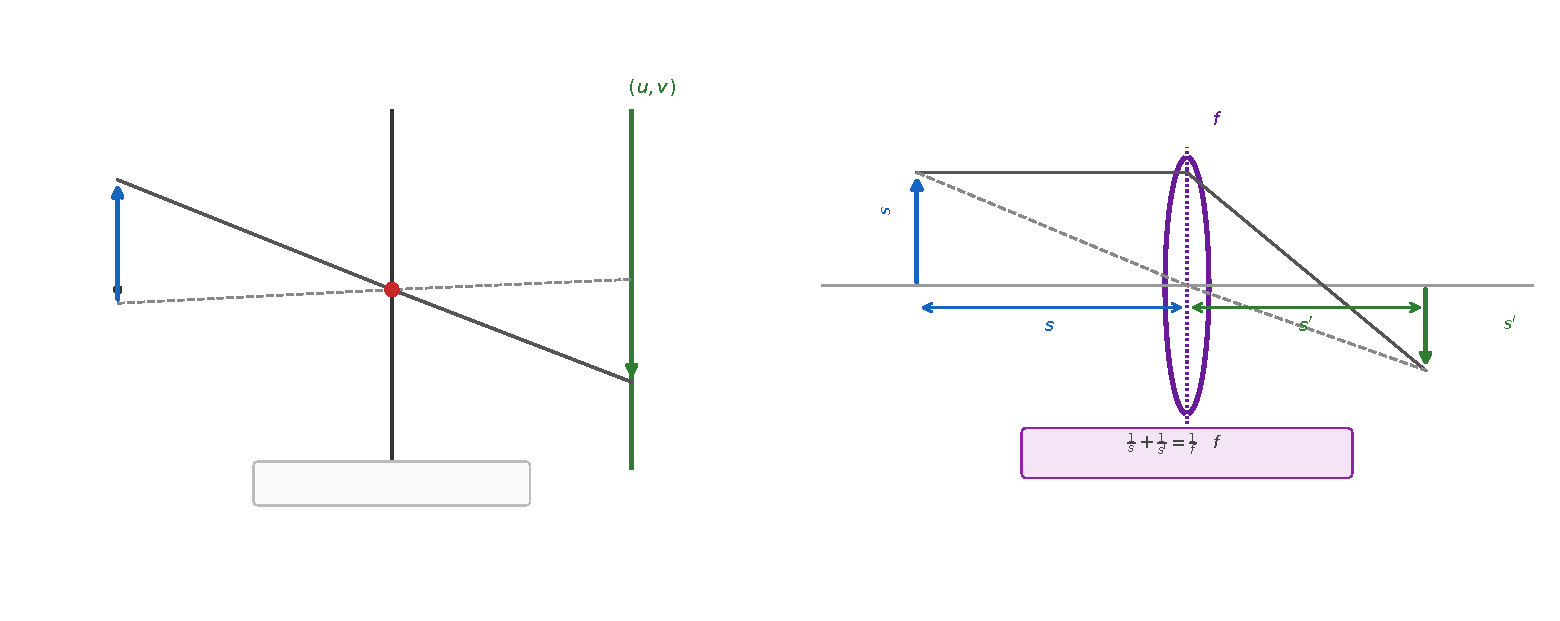
\includegraphics[width=0.95\textwidth]{fig-pinhole-thinlens.pdf}
  \caption{针孔与薄透镜成像概念草图（非精确工程图）。左：光线过针孔，像倒立。右：薄透镜把物距 $s$、像距 $s'$ 与焦距 $f$ 联系起来。}
  \label{fig:ch01-pinhole-thinlens}
\end{figure}

针孔模型\textbf{没有}「对焦」自由度：孔径理想化为点，几何上处处清晰。真实镜头有限孔径，必须引入透镜与离焦——否则无法讨论景深，而这正是近距离医学重建的痛点。

\subsection{薄透镜：对焦与放大率}

旁轴、单色、薄透镜假设下，物距 $s$、像距 $s'$、焦距 $f$ 满足
\begin{equation}
  \frac{1}{s}+\frac{1}{s'}=\frac{1}{f}.
  \label{eq:ch01-thinlens}
\end{equation}
约定：$s,s',f$ 取合适符号约定下的正值讨论（实物、实像、会聚透镜的常见课设约定）；工程实现以厂商与标定文档为准。横向放大率
\[
  m = -\frac{s'}{s}
\]
说明像倒立（负号）且大小由共轭距决定。

\textbf{对焦}在操作上常表现为调节 $s'$（传感器相对镜头的轴向位置）或等效地改变光学组，使给定工作距 $s$ 满足式~\eqref{eq:ch01-thinlens}。对焦不准时，点光源在像面张成弥散斑，而不是式~\eqref{eq:ch01-pinhole} 里的理想点。

有效焦距还会随波长 $\wavelength$ 略变（色散），导致不同颜色的对焦面分离——色差；本章先记一笔，系统展开见 \chapref{ch:08}。折射率 $n$ 进入透镜制造商公式，本书够用层面只需知道：$f$ 由曲率与 $n$ 决定，浸液或窗口玻璃会改共轭关系。

\subsection{有限孔径、弥散圆与景深}

设对焦在物距 $s$，传感器在对应的 $s'$。若物点改到 $s+\Delta s$，理想像面移离传感器，光束在传感器上截出直径为 $c$ 的\textbf{弥散圆}（circle of confusion）。当 $c$ 小于判据 $c_{\max}$（由像素尺寸或可容忍模糊决定）时，该物距仍被视为「可接受清晰」。前后可接受的物距范围，构成景深；文中用 $Z_d$ 统称与景深相关的特征尺度（如景深总长、前/后景深），\textbf{勿}与世界坐标 $Z$ 混用而不加下标。

定性规律（旁轴、常见摄影/机器视觉直觉，精确公式依光圈与放大率而定）：
\begin{itemize}
  \item 容许弥散圆 $c_{\max}$ 越大，表观景深越大；
  \item 相对孔径越大（光圈越大）、焦距 $f$ 越长、放大率越高，景深越窄；
  \item 近距离大放大率（口内、显微）时 $Z_d$ 往往只有毫米量级，牙面起伏即可离焦。
\end{itemize}

\begin{figure}[htbp]
  \centering
  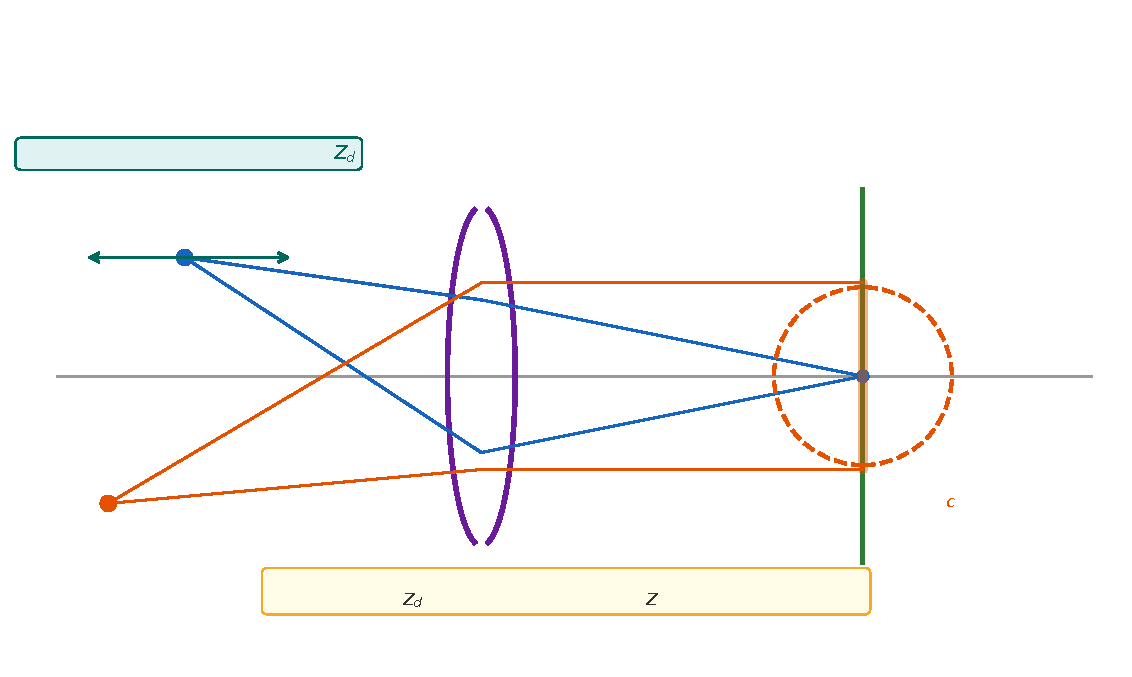
\includegraphics[width=0.92\textwidth]{fig-dof-coc.pdf}
  \caption{景深与弥散圆概念草图。对焦物点在像面收为清晰点；离焦物点张成弥散圆。可接受的物距范围与 $Z_d$ 相关。}
  \label{fig:ch01-dof}
\end{figure}

数值孔径 $\NA$ 在显微与浸液物镜中更常用；与 $f$ 数相关：$F\# \approx 1/(2\NA)$（空气、小角度近似）。$\NA$ 越大，分辨本领往往越好，但景深越窄——分辨率与 $Z_d$ 的折中在 \chapref{ch:03}、\chapref{ch:08} 还会出现。

\subsection{几何畸变：直线不再直}

理想针孔把空间直线投成直线。实际镜头的径向畸变等使像点沿径向伸缩：桶形（中间放大相对小）或枕形（相反）。切向畸变与装配偏心有关。畸变是\textbf{像面坐标的非线性映射}，不能靠提高 $\SNR$ 消除；必须在投影模型中参数化并标定（\chapref{ch:02}）。

对结构光而言：若解码假设「投影行/列对应直线栅」，而相机侧畸变未校正，相位到 $(X,Y,Z)$ 的映射会出现系统性弯曲——点云里牙弓被「掰弯」，常被误诊为算法 bug。

\subsection{从几何光学到计算机视觉投影}

机器视觉把式~\eqref{eq:ch01-pinhole} 像素化：$f$ 以像素计，并加入主点 $(c_x,c_y)$，写成内参 $K$。光学上，$f$ 仍源于像距与透镜；主点接近光轴与传感器交点。外参 $R,t$ 把世界系变到相机系，本身不是光学元件参数，但与标定板姿态、手持扫描轨迹耦合。\citet{HartleyZisserman2004} 给出多视几何全貌；本章要求先建立「$f$、对焦、$Z_d$、畸变」的光学直觉，再进入 \chapref{ch:02} 的矩阵与可观性。


\subsection{物像共轭与「清晰」的操作定义}

工程上说一张图「清晰」，通常指点状特征的能量落在可接受的弥散圆内，而不是数学上的狄拉克点。对结构光，还要在\textbf{条纹空间频带}内保持足够调制度：即使主观看「还行」，高频条纹的对比度仍可能先塌掉。因此同一光圈下，摄影可接受的 $Z_d$ 可以宽于相位测量可接受的 $Z_d$。写设计文档时建议显式给出：
\begin{itemize}
  \item 判据 $c_{\max}$（例如 $1$--$2$ 像素，或与相位误差上限反推）；
  \item 对应的工作距区间与允许探头倾角；
  \item 在该区间内条纹对比度的下限（实测）。
\end{itemize}

\subsection{窗口、浸液与物距的「表观」变化}

保护玻璃、唾液膜或空气–介质界面会使光线折射，等效物距与主面位置偏移。薄透镜公式仍可作\textit{一阶}直觉，但标定得到的有效 $f_x$ 已吸收部分窗口效应；若标定在空气中完成、扫描在另一介质窗口下进行，等于更换了光路却未更换 $K$。医学近距设备务必保证\textbf{标定光路与工作光路一致}（含窗口），否则 \chapref{ch:02} 的可观性讨论会建立在错误的物理上。

\subsection{推导：弥散圆直径与景深公式}

前面给出的是定性规律，这里把它推成可以算数的公式，并写清楚每一步的近似。

\textbf{第一步：轴向放大率。} 对薄透镜式~\eqref{eq:ch01-thinlens} 两边求微分：$-\mathrm{d}s/s^2-\mathrm{d}s'/s'^2=0$，故
\[
  \Delta s'\approx-\frac{s'^2}{s^2}\,\Delta s=-m^2\,\Delta s .
\]
物点沿轴移动 $\Delta s$，像点反向移动 $m^2$ 倍。近距、放大率接近 $1$ 时轴向与横向放大同量级；放大率小（远景）时像点几乎不动，这就是远景景深大的根源。条件：$|\Delta s|\ll s$，一阶展开成立。

\textbf{第二步：相似三角形。} 设入瞳直径 $D=f/N_F$（$N_F$ 为工作 F 数）。会聚到 $s'+\Delta s'$ 的光锥在传感器（位于 $s'$）上截出的圆直径为
\[
  c\approx D\,\frac{|\Delta s'|}{s'}=\frac{f}{N_F}\,\frac{m^2|\Delta s|}{s'} .
\]
条件：$|\Delta s'|\ll s'$，且忽略衍射（第~\ref{ch:03}~章再补）。

\textbf{第三步：反解景深。} 令 $c=c_{\max}$，前后对称近似下总景深
\[
  Z_d\approx 2|\Delta s|_{\max}=\frac{2c_{\max}N_F\,s'}{f\,m^2}.
\]
再用 $s'=f(1+|m|)$（由式~\eqref{eq:ch01-thinlens} 与 $|m|=s'/s$ 得到），最终
\begin{equation}
  Z_d\approx\frac{2\,c_{\max}\,N_F\,(1+|m|)}{m^{2}} .
  \label{eq:ch01-dof}
\end{equation}
这是近摄与机器视觉中常用的景深式。它把定性规律量化了：$Z_d$ 与 $N_F$、$c_{\max}$ 成正比，与 $m^2$ 近似成反比。适用条件：薄透镜、旁轴、$|\Delta s|\ll s$、入瞳与出瞳大小相近（瞳放大率接近 $1$）。远景（$|m|\to0$ 且物距接近超焦距）时前后景深不再对称，此式不适用。

\textbf{例（数量级示意）。} 口内相机看 $15\,\mathrm{mm}$ 宽的视场，传感器宽 $6\,\mathrm{mm}$，故 $|m|=0.4$。像元 $3\,\mu\mathrm{m}$，取 $c_{\max}=2$ 像素 $=6\,\mu\mathrm{m}$。
\begin{itemize}
  \item $N_F=8$：$Z_d\approx2\times0.006\times8\times1.4/0.16\approx0.84\,\mathrm{mm}$；
  \item $N_F=16$：$Z_d\approx1.7\,\mathrm{mm}$。
\end{itemize}
单颗牙的起伏就有数毫米，按「两像素弥散」的判据，几何景深远远不够。这个例子引出两个要在后文回答的问题：其一，缩小光圈换景深会被衍射限制住（像方艾里斑直径约 $2.44\,\lambda N_F(1+|m|)$，$\lambda=450\,\mathrm{nm}$、$N_F=8$ 时约 $12\,\mu\mathrm{m}$，已超过 $c_{\max}$，见第~\ref{ch:03}~章）；其二，结构光并不要求「点」清晰，只要求条纹调制度不塌。对称的模糊只降低正弦条纹的幅度、不移动其相位，所以条纹解码能容忍比角点检测大得多的弥散圆（第~\ref{ch:08}~章用 $\MTF$ 量化）。

\subsection{推导：平板窗口引起的焦点偏移}

口内探头前端常有保护窗或反射镜，显微与内窥中还有盖玻片和浸液。厚度 $t$、折射率 $n$ 的平行平板插在会聚光路中，旁轴近似下会把像点沿轴推远
\[
  \Delta=t\Bigl(1-\frac{1}{n}\Bigr).
\]
推导：光线在平板内折射，入射角 $\theta$ 与折射角 $\theta'$ 满足 $\sin\theta=n\sin\theta'$；穿过平板的横向偏移使光线延长线与轴的交点后移 $t(1-\tan\theta'/\tan\theta)$，旁轴时 $\tan\theta'/\tan\theta\approx1/n$。条件：小角度；大 $\NA$ 时不同孔径带的偏移不同，出现球差。

例：$t=2\,\mathrm{mm}$、$n=1.5$，$\Delta\approx0.67\,\mathrm{mm}$。若标定时没装窗口、扫描时装上，或换了不同厚度的窗口，对焦面与标定内参都会变。这比上面算出的景深还要大，不能忽略。

\section{限度}
\label{sec:ch01-limits}

\begin{itemize}
  \item 旁轴与薄透镜忽略厚透镜主面、场曲、像散等；广角或大视场口内镜头常需更完整模型。
  \item 针孔无衍射：分辨率下限由波动光学给出，$\PSF$/$h$ 与 $\MTF$ 见后续章。
  \item 景深判据 $c_{\max}$ 依赖任务：亚像素相位对模糊比「看看清」更严，故结构光有效 $Z_d$ 往往短于摄影学宣传值。
  \item 畸变模型是近似；极强畸变或非中心投影镜头可能需鱼眼或其他参数化。
\end{itemize}

\section{对象}
\label{sec:ch01-object}

\textbf{场景 A：口内结构光工作距。} 声称景深 $Z_d\approx 10\,\mathrm{mm}$，实际牙尖到沟底高差可达数毫米且探头倾斜。若对焦面设在牙尖，沟底条纹对比度崩溃——点云「顶清底糊」。处置：缩小光圈（换 $\SNR$）、分层对焦融合、或限制姿态使工作距落在 $Z_d$ 内。

\textbf{场景 B：标定板拍得「很锐」但重建弯。} 锐利只说明对焦好；未建模的桶形畸变仍使棋盘格直线弯曲，估出的 $K$ 与射线方向错，三角测量系统性偏。处置：在模型中加径向/切向项并看重投影误差是否各向同性下降。

\textbf{场景 C：把摄影 $f$ 数当算法超参乱调。} 开大光圈提亮却吃掉 $Z_d$；在 CUDA 里加大双边滤波，不如先固定光圈与曝光做光学预算。灰度亮不代表 $E$ 与 $\SNR$ 在条纹频带内够用。


\section*{本章收束}
针孔给出投影骨架，薄透镜给出对焦与 $f$，弥散圆给出 $Z_d$，畸变逼你改模型。把这些写进口内/近距结构光的检查清单后，才能在下一章进入 $K$、畸变参数与标定可观性，而不把矩阵当成纯代数游戏。

\section{习题}
\label{sec:ch01-exercises}

\begin{enumerate}
  \item \textbf{（概念）} 针孔模型为何无法解释「对焦旋钮」？薄透镜模型如何补上？
  \item \textbf{（计算）} 设 $f=12\,\mathrm{mm}$，物距 $s=40\,\mathrm{mm}$。求像距 $s'$。若传感器固定在该 $s'$，物距改为 $45\,\mathrm{mm}$，定性说明像面弥散变大还是变小（不必精确 $c$）。
  \item \textbf{（计算）} 世界点 $(X,Y,Z)=(5,0,100)\,\mathrm{mm}$，针孔 $f=8\,\mathrm{mm}$（单位一致）。求理想像点 $(u,v)$（光心原点、主点在原点）。
  \item \textbf{（重建场景）} 近距扫描中缩小光圈后条纹更「到处都能看清」，但噪声明显变大。用 $Z_d$ 与 $\SNR$ 解释权衡，并给出一条可执行的折中策略。
  \item \textbf{（概念）} 为何说畸变导致的点云弯曲通常不能靠提高曝光消除？
  \item \textbf{（诊断）} 棋盘格照片四角发糊、中心锐：更可能是场曲/像面不理想，还是单纯整体离焦？对标定姿态选择有何启示？
  \item \textbf{（符号）} 文中 $Z_d$ 与深度 $Z$ 同时出现时如何避免混淆？举例写一句正确表述。
  \item \textbf{（推导）} 从式~\eqref{eq:ch01-thinlens} 出发，独立推出轴向放大率 $\Delta s'\approx-m^2\Delta s$，并说明 $|m|=1$ 时它的物理含义。
  \item \textbf{（计算）} 用式~\eqref{eq:ch01-dof}，$|m|=0.2$、$N_F=8$、$c_{\max}=6\,\mu\mathrm{m}$，求 $Z_d$。与正文 $|m|=0.4$ 的结果相比，放大率减半景深变为几倍？代价是什么？
  \item \textbf{（计算）} 正文例中，若要求像方艾里斑直径不超过 $c_{\max}=6\,\mu\mathrm{m}$（$\lambda=450\,\mathrm{nm}$，$|m|=0.4$），$N_F$ 最大取多少？此时几何景深是多少？
  \item \textbf{（口扫场景）} 探头前窗由 $1.0\,\mathrm{mm}$ 换为 $2.0\,\mathrm{mm}$（同为 $n=1.5$），焦点偏移变化多少？给出必须重新做的两件事。
  \item \textbf{（C++/CUDA 实践）} 写出一个函数的接口与内部步骤：输入 $f$、$N_F$、$s$、像元间距与 $c_{\max}$（以像素计），输出前后景深。指出哪一步需要检查适用条件并返回错误。
\end{enumerate}

\section{习题讲解}
\label{sec:ch01-solutions}

\begin{enumerate}
  \item 针孔孔径为零、几何上处处清晰，没有共轭面可调。薄透镜有式~\eqref{eq:ch01-thinlens}，调节 $s'$（或等效）使给定 $s$ 成像在传感器上，即对焦。
  \item $\frac{1}{s'}=\frac{1}{f}-\frac{1}{s}=\frac{1}{12}-\frac{1}{40}=\frac{10-3}{120}=\frac{7}{120}$，故 $s'=\frac{120}{7}\approx17.14\,\mathrm{mm}$。物距变到 $45\,\mathrm{mm}$ 时理想 $s'$ 变小，传感器仍在原处 → 离焦，弥散圆变大。
  \item $u=fX/Z=8\times5/100=0.4\,\mathrm{mm}$，$v=0$。
  \item 小光圈增大 $Z_d$（更处处可接受清晰），但进光少，$\SNR$ 下降，相位/匹配方差升。折中：固定可接受 $Z_d$ 的最大光圈，用曝光时间或增益补 $\SNR$，并防运动模糊；或多曝光融合。
  \item 畸变是几何映射，不随光子数增加而线性校正；曝光主要改 $\SNR$ 与饱和，不改径向多项式形状。
  \item 更像场曲或像差随视场变化，而非单一全局离焦（全局离焦中心也会糊）。标定应覆盖实际工作视场，并检查角点重投影误差是否随半径增大。
  \item 例：「工作距落在景深特征量 $Z_d$ 内时，世界坐标深度 $Z$ 上的点云方差下降。」出现景深时用 $Z_d$，场景深度用 $Z$ 或 $(X,Y,Z)$。
  \item 微分 $1/s+1/s'=1/f$：$-\mathrm{d}s/s^2-\mathrm{d}s'/s'^2=0$，故 $\mathrm{d}s'=-(s'/s)^2\mathrm{d}s=-m^2\mathrm{d}s$。$|m|=1$ 时物点移动多少、像点就反向移动多少，对应 $s=s'=2f$ 的一倍成像。
  \item $Z_d\approx2\times0.006\times8\times1.2/0.04\approx2.9\,\mathrm{mm}$，约为 $|m|=0.4$ 时 $0.84\,\mathrm{mm}$ 的 $3.4$ 倍（$(1+|m|)/m^2$ 之比 $30/8.75$）。代价：同样传感器视场变大、物方每像素对应更大尺寸，$f_x$ 对应的物方分辨率下降，同样 $\delta d$ 带来的横向误差变大。
  \item $2.44\times0.45\,\mu\mathrm{m}\times N_F\times1.4\le6\,\mu\mathrm{m}$，得 $N_F\le3.9$，取 $N_F\approx4$。此时 $Z_d\approx2\times0.006\times4\times1.4/0.16\approx0.42\,\mathrm{mm}$。在这个放大率和像素下，「几何清晰」与「衍射清晰」同时满足时景深只有约 $0.4\,\mathrm{mm}$，说明必须放宽判据（依靠条纹对模糊的容忍）而不是一味缩光圈。
  \item 偏移由 $0.33\,\mathrm{mm}$ 变为 $0.67\,\mathrm{mm}$，变化约 $0.33\,\mathrm{mm}$，与景深同量级。必须：重新对焦（或确认对焦面仍覆盖工作距）；在新窗口下重新标定内参与畸变（大 $\NA$ 时窗口还引入球差）。
  \item 接口：输入 \texttt{f\_mm}、\texttt{NF}、\texttt{s\_mm}、\texttt{p\_mm}、\texttt{cmax\_px}，输出 \texttt{near\_mm}、\texttt{far\_mm}。步骤：(1) $s'=fs/(s-f)$，检查 $s>f$；(2) $|m|=s'/s$；(3) $c_{\max}=c_{\max,\mathrm{px}}\cdot p$；(4) $|\Delta s|=c_{\max}N_Fs'/(fm^2)$；(5) 检查 $|\Delta s|\ll s$（如小于 $0.1s$），否则返回「一阶近似失效」或改用精确前后景深公式。单位全部用毫米，像素只在输入处换算一次。
\end{enumerate}

\chapter{相机投影几何的光学约束}
\label{ch:02}

\section{效果}
\label{sec:ch02-effect}

读完本章，你应能：
\begin{enumerate}
  \item 写出含内参矩阵 $K$ 的投影模型，并解释 $f_x,f_y$、主点与像素尺度的光学来源；
  \item 在针孔投影上叠加径向/切向畸变，说明校正顺序与重投影误差的含义；
  \item 陈述景深 $Z_d$ 如何限制「可用于标定与重建的清晰工作距」，以及模糊对特征定位的影响；
  \item 从可观性角度判断：哪些运动与板姿态能把 $K$、畸变与外参 $R,t$ 分开估准，哪些配置会退化。
\end{enumerate}

\section{原理}
\label{sec:ch02-principle}

\subsection{内参 $K$：把光学焦距写成矩阵}

相机坐标系下，点 $\mathbf{X}_c=(X,Y,Z)^\top$（$Z>0$ 在镜头前方的常见约定）先按针孔投影到归一化像平面，再乘内参。像素齐次坐标常写为
\begin{equation}
  s\begin{pmatrix}u\\v\\1\end{pmatrix}
  =
  K\begin{pmatrix}X\\Y\\Z\end{pmatrix},
  \qquad
  K=\begin{pmatrix}f_x & 0 & c_x\\ 0 & f_y & c_y\\ 0&0&1\end{pmatrix},
  \label{eq:ch02-K}
\end{equation}
其中 $s$ 为齐次尺度（齐次因子）。非齐次形式更直观：
\[
  u = f_x\frac{X}{Z}+c_x,\qquad
  v = f_y\frac{Y}{Z}+c_y
  \quad(Z\neq 0).
\]
$f_x,f_y$ 是以像素计的焦距，近似 $f/p_x$、$f/p_y$（$f$ 为毫米焦距，$p_x,p_y$ 为像素间距）；$c_x,c_y$ 为主点，理想上接近光轴与传感器交点的像素坐标。斜歪参数（skew）在现代传感器上常可置零。

光学约束体现在：
\begin{itemize}
  \item $f_x\approx f_y$ 通常接近（方形像素）；显著差异可能来自错误标定或非对称光学；
  \item 主点偏离中心过大时，应怀疑装配、裁切或模型与镜头不匹配；
  \item $K$ 把「毫米光路」接到「像素算法」；$K$ 错则所有三角测量的射线方向错。
\end{itemize}

世界系到相机系：$\mathbf{X}_c=R\mathbf{X}+t$，外参 $R,t$ 描述刚体位姿。多视几何与标定算法见 \citet{HartleyZisserman2004}；平面靶实用流程见 \citet{Zhang2000Calibration}。

\subsection{畸变模型：在归一化平面上改弯}

常用做法：先将像素反投影到归一化坐标 $(x,y)$（未畸变），再施加畸变得到 $(\tilde{x},\tilde{y})$，最后用 $K$ 映回像素——或按实现库的约定顺序严格一致。径向模型示意：
\begin{equation}
  \begin{pmatrix}\tilde{x}\\\tilde{y}\end{pmatrix}
  =
  (1+k_1 r^2+k_2 r^4+\cdots)
  \begin{pmatrix}x\\y\end{pmatrix}
  +\text{切向项},
  \qquad r^2=x^2+y^2.
  \label{eq:ch02-dist}
\end{equation}
$k_1<0$ 常对应桶形倾向，$k_1>0$ 常对应枕形倾向（符号约定因库而异，以文档为准）。切向项刻画偏心等。

\begin{figure}[htbp]
  \centering
  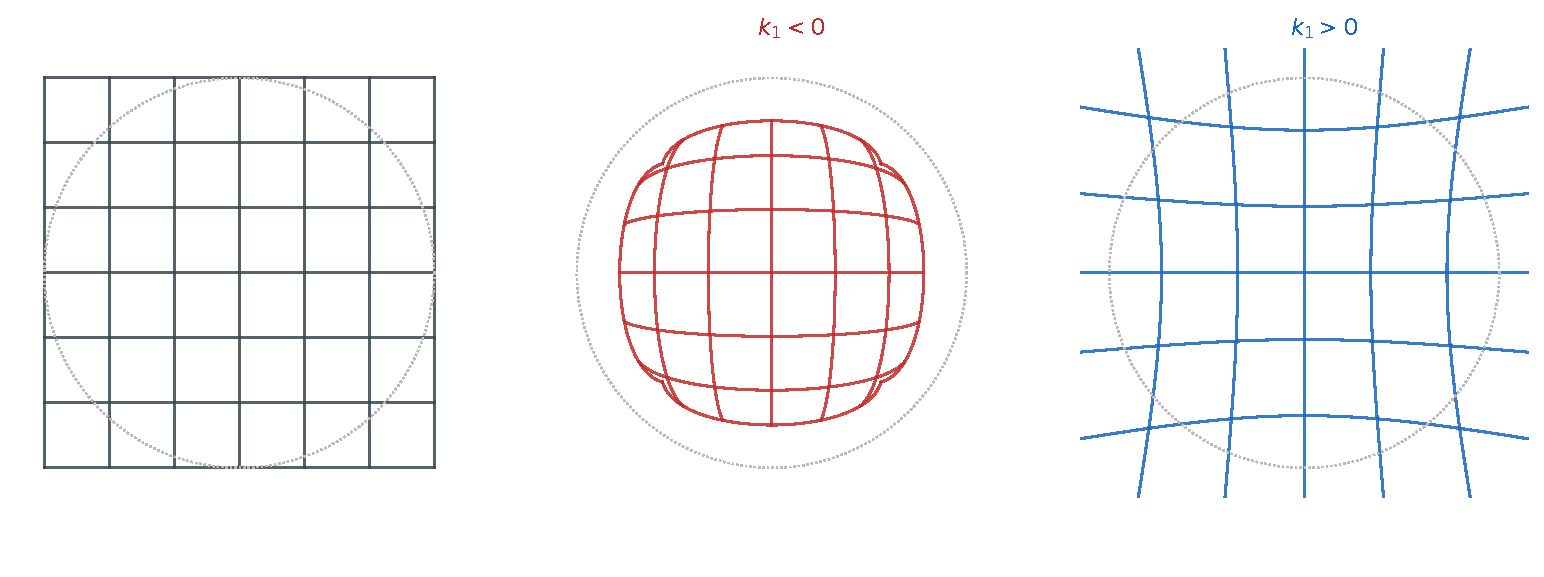
\includegraphics[width=0.95\textwidth]{fig-distortion.pdf}
  \caption{理想网格与桶形/枕形径向畸变概念草图（非精确工程图）。直线在像面上变弯，必须在投影模型中显式建模。}
  \label{fig:ch02-distortion}
\end{figure}

\textbf{重投影误差}：三维点（或标定板上的已知点）经 $R,t$、畸变与 $K$ 预测像素，与检测角点之差。优化标定即减小该类误差。若模型不含畸变，误差会呈径向结构；强行只用 $K$ 会把弯曲「吞进」错误的 $f_x,f_y$ 或主点，留下系统性点云变形。

\subsection{景深、模糊与特征定位}

标定与重建都依赖特征（角点、条纹峰值）的亚像素定位。离焦使 $\PSF$ 展宽，角点响应变钝，定位方差上升；条纹对比度下降等价于频带内 $\SNR$ 变差。因此存在光学约束：
\begin{quote}
有效数据必须落在由 $c_{\max}$ 决定的景深范围（用 $Z_d$ 表征）内；否则估出的 $K$ 或相位是「糊图上的最佳拟合」，泛化到清晰工作距时失效。
\end{quote}
近距大视场时，场曲还会让中心与边缘不能同时最锐（\chapref{ch:01}），标定姿态应覆盖实际扫描的工作距与视场，而非只追求中心一块极锐。

\subsection{标定可观性：什么运动能把参数分开}

平面靶标定 \citep{Zhang2000Calibration} 需要多幅不同姿态。可观性直觉：
\begin{itemize}
  \item \textbf{足够透视变化}：靶面不可总与像面平行且距离不变，否则焦距与深度尺度易纠缠；
  \item \textbf{覆盖视场}：角点应伸到边缘，否则高阶畸变 $k_2,\ldots$ 不可观或过拟合噪声；
  \item \textbf{$Z_d$ 内清晰}：每幅用于标定的图都必须在可接受弥散内；
  \item \textbf{外参与内参}：单目序列中 $R,t$ 每幅不同，$K$ 共享；若错误地让 $K$ 随时间漂，属于过参数化；
  \item \textbf{退化}：所有图像共面运动、视场中央一小块、或几乎纯旋转且无已知尺度时，部分参数方差爆炸。
\end{itemize}

结构光系统还常标定投影仪–相机相对 $R,t$ 与投影仪「内参」。投影仪可类比倒装的相机：其「畸变」与离焦同样存在；条纹相位到射线的映射继承这些误差，并在三角测量中放大（\chapref{ch:07}）。

\subsection{与光学公式的交接}

像素焦距 $f_x$ 随对焦轻微变化（像距 $s'$ 变）；自动对焦扫描头若对焦后仍用旧 $K$，等于系统性改射线方向。浸液、保护窗、温度引起的 $n$ 与机械间隙变化，也会让出厂 $K$ 漂移。工程上：关键工况下定期重标定，并监控重投影误差与点云金标准偏差，而不是假定 $K$ 永恒。


\subsection{从重投影误差到点云误差的数量级直觉}

设角点或相位对应点的像面定位误差为 $\delta u$ 像素，焦距约 $f_x$ 像素，工作距深度 $Z$，基线为 $B$（双目或相机–投影中心距）。三角测量下深度误差常有
\[
  \delta Z \;\sim\; \frac{Z^{2}}{B f_x}\,\delta u
\]
量级关系（系数因几何定义略有不同）。含义：
\begin{itemize}
  \item 同样 $\delta u$，更远或更短基线 → $\delta Z$ 更大；
  \item 离焦或畸变未建模会抬高有效 $\delta u$，并可能引入\textbf{与半径相关的系统} $\delta u$，于是点云出现可重复的弯曲而非仅方差增大；
  \item 标定把 $\delta u$ 的系统部分压下去，比在点云端做各向同性平滑更对症。
\end{itemize}
完整立体限度见 \chapref{ch:07}；本章要求先承认：\textbf{$K$ 与畸变的光学约束通过 $\delta u$ 进入 $\delta Z$}。

\subsection{实现提示（C++/CUDA 视角）}

\begin{itemize}
  \item 畸变校正与投影的顺序必须与标定库一致；在 CUDA 里自写反畸变迭代时，用标定板角点做端到端金标准测试。
  \item 不要把「查找表校正后的图」再送进假定「未校正」的第二套模型。
  \item 对焦电机位置若可读，应记入元数据；任一档位对应一套 $K$ 或一套放大率，禁止混用。
  \item 监控项：每批次标定的重投影 RMS、边缘 vs 中心误差比、以及已知长度量块随 $Z$ 的尺度曲线。
\end{itemize}

\section{限度}
\label{sec:ch02-limits}

\begin{itemize}
  \item 式~\eqref{eq:ch02-K}--\eqref{eq:ch02-dist} 是常用工程模型，不是透镜设计的完整像差展开。
  \item 可观性讨论是定性的；定量协方差依赖角点噪声模型与姿态分布，需用实际标定报告或仿真确认。
  \item 忽略畸变的「也能跑」的 $K$ 在窄视场、弱畸变镜头上可勉强；口内广角常见强畸变，此限度不可忽略。
\end{itemize}

\section{对象}
\label{sec:ch02-object}

\textbf{诊断 1：点云整体「球面感」或边缘外翻。} 先可视化标定板直线是否弯曲、重投影误差是否随半径增大。若是，增强畸变阶数或检查是否用了错误的畸变约定（像素域 vs 归一化域）。对照图~\ref{fig:ch02-distortion} 理解桶/枕方向与 $k_1$ 符号。

\textbf{诊断 2：金标准长度随工作距变化。} 可疑 $f_x,f_y$ 与深度耦合、或对焦后 $K$ 未更新，或窗口玻璃未建模型。在多个 $Z$ 上拍靶，看尺度误差是否单调。

\textbf{诊断 3：标定重投影很小，实地扫描仍差。} 可能标定姿态未覆盖扫描时的 $Z_d$ 与视场（过拟合中心清晰区）；或外参 $R,t$ 在装配后被碰撞改变。用「扫描工况下的再投影 / 再标定」验证，而非只看实验室最优图。

\textbf{诊断 4：左右相机相对位姿不稳。} 双目 $R,t$ 误差直接放大深度；光学上还要保证两路均在 $Z_d$ 内且光照 $\SNR$ 对称，否则匹配偏差被当成几何。


\section*{本章收束}
$K$ 把毫米光路接到像素；畸变在归一化平面改弯；$Z_d$ 约束哪些图能进标定；姿态设计决定可观性。重投影误差与 $\delta Z\sim Z^2\delta u/(B f_x)$ 量级把光学约束接到点云。本编几何与相机部分到此；波动与光度线索从 \chapref{ch:03} 起展开。

\section{习题}
\label{sec:ch02-exercises}

\begin{enumerate}
  \item \textbf{（概念）} 解释 $f_x$ 与薄透镜焦距 $f$（毫米）的关系；像素变小（传感器更密）时，同样光学 $f$ 下 $f_x$ 如何变？
  \item \textbf{（计算）} 设 $f_x=f_y=800$（像素），$c_x=640$，$c_y=360$。相机系点 $(X,Y,Z)=(10,0,200)$（单位任意但一致）。忽略畸变，求像素 $(u,v)$。
  \item \textbf{（计算）} 归一化坐标 $(x,y)=(0.3,0.0)$，$r^2=0.09$，仅径向 $k_1=-0.2$（其余为零）。求畸变后的 $(\tilde{x},\tilde{y})$。相对无畸变，像点更靠近还是更远离中心？
  \item \textbf{（可观性）} 只拍三张几乎平行、距离相同的标定板图像，主要哪类参数难估准？应如何改采集？
  \item \textbf{（重建场景）} 口内头对焦在 $s=25\,\mathrm{mm}$ 后标定；扫描时对焦环被扳到 $s=30\,\mathrm{mm}$ 但未重标。定性预测深度误差类型，并给出处置。
  \item \textbf{（诊断）} 重投影误差中心 $<0.1$~px、四角 $>1$~px，且呈径向。优先加畸变项还是提高角点检测窗口？
  \item \textbf{（综合）} 为何说「景深 $Z_d$」是标定的光学约束而非纯软件选项？举一条违反后的失败模式。
\end{enumerate}

\section{习题讲解}
\label{sec:ch02-solutions}

\begin{enumerate}
  \item $f_x\approx f/p_x$。像素间距 $p_x$ 变小则同样毫米焦距对应更大的 $f_x$（更多像素）。
  \item $u=f_x X/Z+c_x=800\times10/200+640=40+640=680$，$v=c_y=360$。
  \item 因子 $1+k_1 r^2=1-0.2\times0.09=0.982$，故 $(\tilde{x},\tilde{y})=(0.2946,0)$，更靠近中心（桶形倾向示意）。
  \item 焦距与深度尺度、部分畸变可观性差。应改变倾斜角与距离，让透视变化明显，并让角点覆盖边缘。
  \item 像距变化使有效 $f_x,f_y$ 与清晰面改变，射线方向与工作距模型偏离，深度出现与 $Z$ 相关的系统偏差。处置：对焦锁定或对焦后重标；禁止静默扳对焦环。
  \item 优先加/检畸变模型与阶数；单纯加大检测窗口不能消除径向结构系统差。
  \item 标定优化默认特征定位无偏；若图在 $Z_d$ 外，定位偏且糊，得到的 $K$ 不代表清晰工况。失败模式：实验室糊图上误差「还行」，实地清晰扫描边缘点云系统性外翻。
\end{enumerate}

\chapter{波动光学够用本}
\label{ch:03}

\section{效果}
\label{sec:ch03-effect}

读完本章，你应能：
\begin{enumerate}
  \item 用双光束干涉解释条纹强度如何随相位 $\varphi$（或光程差 $\OPD$/$\opd$）变化，并写出可见度 $V$ 的含义；
  \item 陈述相干长度的够用直觉：何时还能看见稳定干涉，何时条纹被「洗掉」；
  \item 把衍射极限、艾里斑与点扩散函数 $\PSF$（记 $h$）联系起来，说明分辨率与数值孔径 $\NA$、波长 $\wavelength$ 的折中；
  \item 在结构光场景中诊断：条纹对比度塌陷究竟更像离焦、衍射截止，还是光源相干/带宽问题。
\end{enumerate}

\section{原理}
\label{sec:ch03-principle}

\subsection{从几何光线到相位}

第~\ref{ch:01}~章的针孔与薄透镜回答「光线往哪走」。结构光与干涉测量还要问：两束光在像面某点的\textbf{相位差}是多少。单色平面波的相位沿传播积累；两路光程之差记为光程差 $\OPD$（亦常用 $\opd$），与相位的关系为
\begin{equation}
  \varphi = \frac{2\pi}{\wavelength}\,\opd
  \quad\text{（或}\ \varphi=\tfrac{2\pi}{\wavelength}\,\OPD\text{）}.
  \label{eq:ch03-phase-opd}
\end{equation}
记号锁定：$\wavelength$ 只表示波长；光学频率为 $\nuopt$（满足 $c=\wavelength\nuopt$ 在真空中）；焦距仍是 $f$，绝不用 $f$ 表示频率。

\subsection{双光束干涉与条纹}

设两束相干光在观察点的复振幅相加，平均强度（辐射度量语境下更接近辐照度时用 $E$，本章谈干涉条纹时沿用强度 $I$ 并注明）可写成
\begin{equation}
  I = I_1+I_2+2\sqrt{I_1 I_2}\,\lvert\gamma\rvert\cos\varphi,
  \label{eq:ch03-twobeam}
\end{equation}
其中 $\varphi$ 含几何相位与可能的初始相位；$\lvert\gamma\rvert$ 概括相干程度（完全相干时取 $1$ 的理想化）。若 $I_1=I_2=I_0/2$，则
\begin{equation}
  I = I_0\bigl(1+V\cos\varphi\bigr),
  \qquad
  V=\frac{I_{\max}-I_{\min}}{I_{\max}+I_{\min}}.
  \label{eq:ch03-visibility}
\end{equation}
$V$ 称为条纹可见度（对比度）。$V\to0$ 时条纹消失，相位无法从强度中稳健估计——这正是结构光解码失败的常见光学原因之一 \citep{HechtOptics,BornWolf}。

\begin{figure}[htbp]
  \centering
  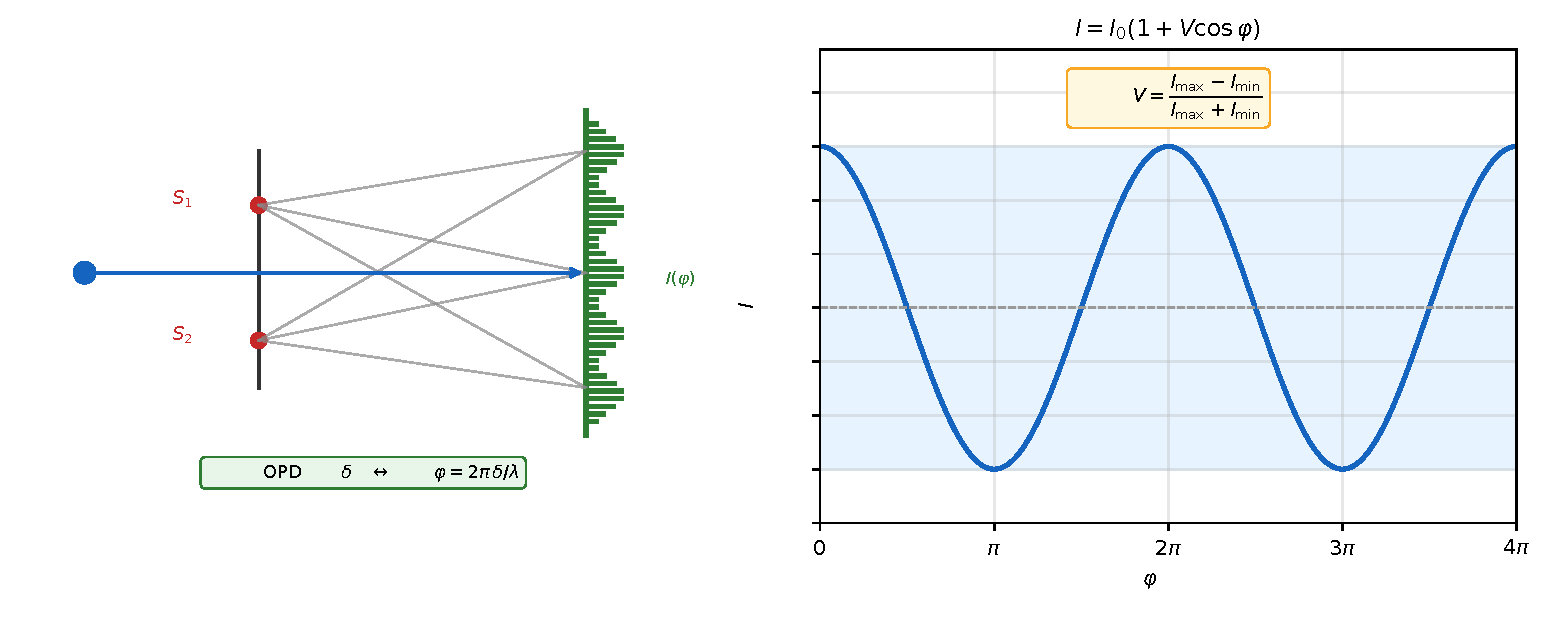
\includegraphics[width=0.95\textwidth]{fig-interference-twobeam.pdf}
  \caption{双光束干涉概念草图（非精确工程图）。左：双路到屏上形成条纹；右：强度随相位振荡，振幅由可见度 $V$ 决定。}
  \label{fig:ch03-interference}
\end{figure}

杨氏双缝给出空间条纹；分振幅干涉（薄膜、迈克尔逊等）给出随光程扫描的条纹。结构光投影仪把「已知空间相位编码」投到物体上，相机记录的是经表面反射/散射后的\textbf{调制度图案}；其可解码性首先要求 $V$ 足够大，其次才是算法。

\subsection{相干长度：够用直觉}

真实光源有频谱宽度。频谱越宽，不同频率成分的干涉条纹错位叠加，有效可见度随光程差增大而下降。相干长度 $\ell_c$ 可粗估为
\begin{equation}
  \ell_c \;\sim\; \frac{\wavelength^{2}}{\Delta\wavelength},
  \label{eq:ch03-coherence-length}
\end{equation}
其中 $\Delta\wavelength$ 为有效光谱宽度（数量级关系，精确定义依频谱形状）。当 $|\OPD|\ll\ell_c$ 时，干涉仍可清晰；当 $|\OPD|$ 接近或超过 $\ell_c$，条纹被冲刷。LED、滤波宽带源、激光的 $\ell_c$ 可差多个数量级：激光易得高 $V$，但也更易在粗糙面上产生散斑（第~\ref{ch:04}~章）。

对「投影正弦条纹 + 相机成像」的主动光测量：光源往往只需\textbf{时间/空间部分相干}到能在相机积分时间内保持稳定图案；并非处处需要实验室级长相干。但若你做的是真干涉测距或光谱敏感的外差，相干长度就变成硬约束。

\subsection{衍射、艾里斑与分辨率}

有限孔径使理想点物的像不再是几何点，而呈衍射图案。圆孔远场的艾里斑中，第一暗环角半径约为
\begin{equation}
  \theta \;\approx\; 1.22\,\frac{\wavelength}{D},
  \label{eq:ch03-airy}
\end{equation}
$D$ 为孔径。物镜侧常用数值孔径 $\NA=n\sin\alpha$；瑞利分辨距离量级为 $0.61\wavelength/\NA$（浸液时 $n>1$ 可缩小）。更大 $\NA$ 提高横向分辨率，同时往往\textbf{压缩景深}（与第~\ref{ch:01}~章 $Z_d$ 的权衡一致）。

\subsection{点扩散函数 $\PSF$ 与 $\MTF$}

线性空不变成像下，像是物与点扩散函数 $h$（即 $\PSF$）的卷积。离焦、像差、衍射都使 $h$ 展宽。其频域传递为光学传递函数；模即为调制传递函数 $\MTF$：空间频率越高，调制度保留越少 \citep{GoodmanFourierOptics}。因此：
\begin{itemize}
  \item 条纹空间频率越高，越容易被 $\MTF$ 杀掉对比度；
  \item 离焦使 $\MTF$ 更早截止，表现为「条纹发灰、相位方差爆」；
  \item 像素采样还需满足奈奎斯特：光学截止与采样截止共同限制可用频率。
\end{itemize}

\begin{figure}[htbp]
  \centering
  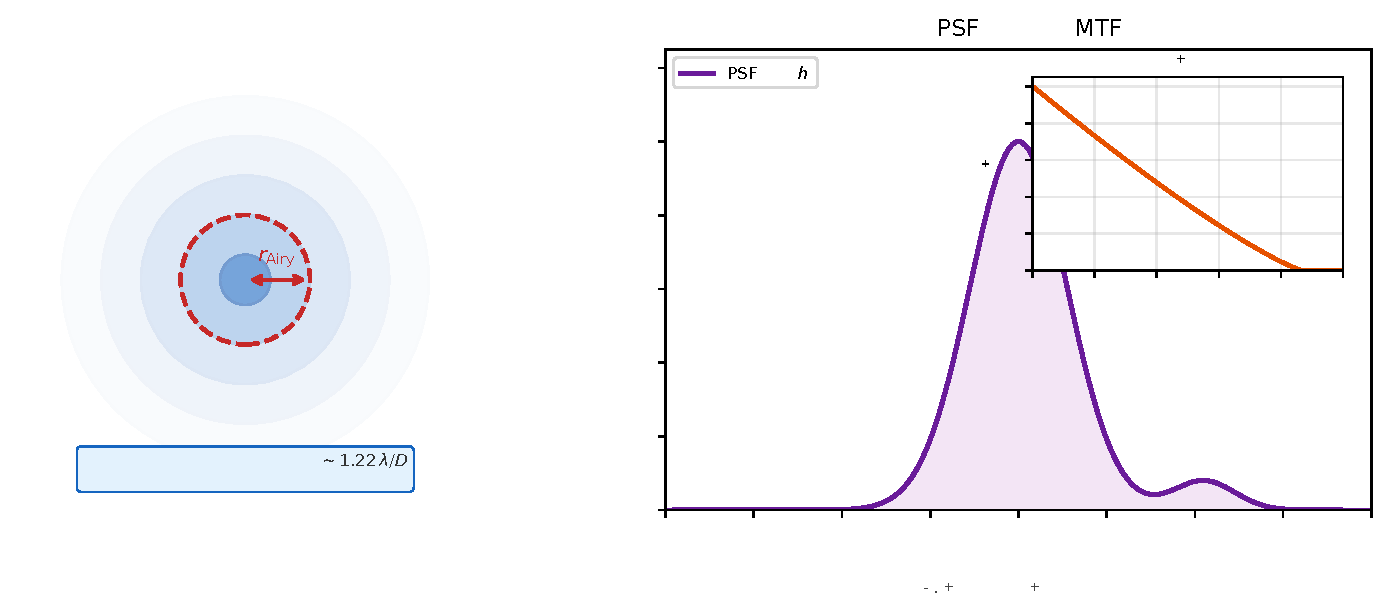
\includegraphics[width=0.95\textwidth]{fig-diffraction-psf.pdf}
  \caption{衍射极限艾里斑与 $\PSF$/$\MTF$ 概念草图（非精确工程图）。高频调制度先丢失，直接威胁细条纹与细纹理。}
  \label{fig:ch03-psf}
\end{figure}

\subsection{与重建分辨率的对接}

深度或形状分辨率往往\textbf{不是}「艾里斑直径直接写在点云上」。结构光里，相位估计精度大致随 $V$ 与 $\SNR$ 改善；三角测量再把像面误差放大为 $\delta Z$（第~\ref{ch:02}~章量级关系）。衍射与离焦同时抬高有效定位误差并降低 $V$，二者叠加。细纹理立体匹配同样吃 $\MTF$：纹理频谱落在截止外就无法匹配。

相位展开与解缠算法（如 \cite{GhigliaPritt1998}）假定条纹可辨；光学上已经 $V\approx0$ 的区域，再强的解缠也只是在噪声上作图。


\subsection{空间频率：条纹要落在系统通带内}

把投影条纹近似为像面上的余弦图案，其空间频率为 $\xi$（线对/毫米或周期/像素）。只有当 $\xi$ 落在光学 $\MTF$ 与传感器采样通带的交集内，调制度才以可见的 $V$ 到达解码器。提高 $\xi$ 本意是加密相位缠绕、提高深度灵敏度，但一旦越过截止，$V$ 崩溃，灵敏度反而变差。多频结构光的「低频保展开、高频提精度」正是在通带与解缠之间做调度：低频更耐离焦与衍射衰减。

采样侧：若每条纹周期少于约 $2$--$3$ 像素（再计非线性与噪声，实务常留更多余量），离散化本身就损 $V$。光学模糊核宽度 $\sigma_{h}$ 与条纹周期 $\Lambda$ 之比 $\sigma_{h}/\Lambda$ 是一个好用的无量纲诊断：比值增大时，先降频或先收锐对焦，而不是先改 CUDA 里的解缠参数。

\subsection{时间积分与振动}

相机曝光时间 $\tau$ 内若光程差或条纹相位因振动漂移 $\Delta\varphi(\tau)$，等价于对 $\cos\varphi$ 做时间平均，有效 $V$ 再乘一个衰减因子。手持口内扫描的微颤、投影风扇、地板振动，都会在高倍率、长相干架构里变成可见度杀手。短曝光提高瞬时锐度，但掉 $\SNR$（第~\ref{ch:05}~章）；脉冲照明与全局快门是光学–电子协同手段。

\section{限度}
\label{sec:ch03-limits}

\begin{itemize}
  \item 式~\eqref{eq:ch03-twobeam}--\eqref{eq:ch03-airy} 是标量、旁轴、够用模型；矢量偏振、严格电磁散射见深入教材 \citep{BornWolf}。
  \item 相干长度公式为数量级；LED 光谱非矩形时需用相干函数更细致描述。
  \item 「衍射极限」不保证系统达到该极限：像差、抖动、传感器采样常先成为瓶颈。
  \item 本章不展开完整傅里叶光学推导；需要传递函数设计时读 \cite{GoodmanFourierOptics}。
\end{itemize}

\section{对象}
\label{sec:ch03-object}

\textbf{结构光条纹对比度。} 正弦条纹投到牙面后相机所见 $V$ 不足：先分清——(1) 整体离焦/$Z_d$ 不够 → $\PSF$ 展宽、$\MTF$ 下降；(2) 条纹频率相对孔径与像素过高 → 衍射+采样截止；(3) 光源有效 $\Delta\wavelength$ 大且两路 $\OPD$ 大 → 相干冲刷（真干涉架构更常见）。提高投影亮度只改善光子 $\SNR$，\textbf{不}自动修复截止频率以外的调制度。

\textbf{离焦模糊。} 沟窝相对对焦面偏移时，局部 $V(u,v)$ 塌陷，相位图呈斑驳；点云在高频形貌处空洞。处置：收光圈换 $Z_d$（付 $\SNR$ 代价）、分层对焦，或降低条纹频率并改用多频策略。

\textbf{衍射对细纹理的限度。} 极细釉质裂纹或加工刀痕，其空间频率可能落在系统 $\MTF$ 之外：立体匹配失锁、结构光边缘相位偏置。这是物理分辨率预算，不是单纯「再训一个网络」能取消的。


\textbf{细条纹选型检查表。} 上线新条纹频率前，固定工作距与光圈，拍摄平面漫射靶：测量像面条纹周期（像素）与调制幅度；把频率逐步提高直到 $V$ 掉到预设阈值（例如低于 $0.3$），该频率即通带边缘。产品条纹应离边缘留裕量，因为牙面离焦与场曲还会再吃掉 $\MTF$。

\section*{本章收束}
干涉给出 $\varphi$ 与 $V$，相干长度约束何时有条纹，衍射与 $\PSF$/$\MTF$ 约束细条纹能否通过。结构光对比度问题应先问通带与离焦，再问算法。偏振与散斑将在第~\ref{ch:04}~章展开；通量与 $\SNR$ 在第~\ref{ch:05}~章展开。

\section{习题}
\label{sec:ch03-exercises}

\begin{enumerate}
  \item \textbf{（概念）} 为何条纹可见度 $V\to0$ 时，相位 $\varphi$ 难以从单像素强度估计？与「图像整体仍然很亮」是否矛盾？
  \item \textbf{（计算）} 两束等强完全相干，$I_0=100$（相对单位），$V=1$，$\varphi=\pi/2$。求 $I$。若 $V$ 降为 $0.2$ 而其余不变，$I$ 如何变？
  \item \textbf{（计算）} 中心波长 $\wavelength=550\,\mathrm{nm}$，有效 $\Delta\wavelength=20\,\mathrm{nm}$。粗估相干长度 $\ell_c$。若系统 $\OPD=0.5\,\mathrm{mm}$，条纹是否容易被冲刷？
  \item \textbf{（计算）} 孔径 $D=4\,\mathrm{mm}$，$\wavelength=550\,\mathrm{nm}$。用式~\eqref{eq:ch03-airy} 估角半径 $\theta$（弧度）。若像距约 $20\,\mathrm{mm}$，艾里斑半径量级（毫米）大约多少？
  \item \textbf{（重建场景）} 提高投影条纹频率后，中心对比度尚可、视场边缘条纹几乎消失。更可能是畸变模型错误，还是边缘 $\MTF$/相对孔径问题？给出检查顺序。
  \item \textbf{（重建场景）} 口内扫描沟底相位噪声大、牙尖正常。用 $Z_d$、$\PSF$、$V$ 写四步诊断。
  \item \textbf{（综合）} 激光照明 $V$ 很高但点云出现颗粒状抖动；LED 照明更平滑但对比度略低。这分别指向哪类波动/相干现象？（散斑细节见第~\ref{ch:04}~章。）
\end{enumerate}

\section{习题讲解}
\label{sec:ch03-solutions}

\begin{enumerate}
  \item $I=I_0(1+V\cos\varphi)$ 对 $\varphi$ 的灵敏度正比于 $V$。$V\to0$ 时 $I$ 对 $\varphi$ 几乎不变，无法反演。可以整体很亮（$I_0$ 大）但毫无调制，二者不矛盾。
  \item $I=I_0(1+V\cos\varphi)=100(1+1\cdot0)=100$。$V=0.2$ 时仍为 $100$（因 $\cos\pi/2=0$）。可见度改变的是极值差，不改变该相位点的瞬时 $I$；估计方差仍会因 $V$ 下降而变差。
  \item $\ell_c\sim\wavelength^{2}/\Delta\wavelength=(550\times10^{-9})^{2}/(20\times10^{-9})\approx15\,\mu\mathrm{m}$。$\OPD=0.5\,\mathrm{mm}\gg15\,\mu\mathrm{m}$，真干涉条纹极易被冲刷。普通投影纹理成像不依赖如此大的相干光程差。
  \item $\theta\approx1.22\times550\times10^{-9}/4\times10^{-3}\approx1.68\times10^{-4}\,\mathrm{rad}$。线半径 $\sim\theta s'\approx1.68\times10^{-4}\times20\approx3.4\,\mu\mathrm{m}$ 量级（概念估算）。
  \item 更优先查边缘照度、斜光束与局部离焦导致的 $\MTF$ 下降，以及相对孔径；畸变造成几何弯曲但不必先「消灭对比度」。顺序：看原图边缘 $V(u,v)$ → 查对焦场曲 → 再查曝光与投影均匀性 → 最后才怀疑纯几何标定。
  \item (1) 沟底是否超出 $Z_d$；(2) 局部 $\PSF$ 是否明显宽于牙尖；(3) 条纹局部 $V$ 是否塌；(4) 再查运动模糊与湿润高反（光度/偏振）。先光学后算法。
  \item 激光：高相干 → 粗糙面散斑，相位/匹配出现颗粒噪声。LED：较短相干、较少散斑，但可能较低 $V$ 或较低通量。需在散斑与对比度之间做光源选型折中。
\end{enumerate}

\chapter{偏振与部分相干}
\label{ch:04}

% TODO: 核心「为什么要懂」— 投影机/相机偏光片、对比度、散斑

\section{效果}
\label{sec:ch04-effect}
% TODO: 读完本章应能回答什么（条目化，落到重建场景）

\section{原理}
\label{sec:ch04-principle}
% TODO: 主流光学教程习惯下的够用展开；公式适度

\section{限度}
\label{sec:ch04-limits}
% TODO: 假设边界、失效模式、与重建误差的关系

\section{对象}
\label{sec:ch04-object}
% TODO: 必须落到相机/投影/干涉/条纹/重建误差中的具体场景

\section{习题}
\label{sec:ch04-exercises}
% TODO: 4–8 题（概念 + 计算 + 重建场景设计/诊断）；至少一半对应相机/投影/条纹/点云误差

\section{习题讲解}
\label{sec:ch04-solutions}
% TODO: 章末讲解（不另开总附录）

\chapter{偏振与部分相干}
\label{ch:05}

\section{效果}
\label{sec:ch04-effect}

读完本章，你应能：
\begin{enumerate}
  \item 说明线偏光、检偏与马吕斯定律如何改变到达相机的通量，以及这与「对比度」而非单纯「变暗」的关系；
  \item 区分完全相干、非相干与部分相干对干涉可见度 $V$ 的影响，并联系第~\ref{ch:04}~章的相干长度直觉；
  \item 解释粗糙表面在高相干照明下为何出现散斑，散斑如何抬高相位/匹配误差；
  \item 在高反牙面、金属器械、投影仪–相机光路中，设计「是否加偏振片」的利弊账（对比度 vs $\SNR$）。
\end{enumerate}

\section{原理}
\label{sec:ch04-principle}

\subsection{偏振态：够用语言}

光波电场振动方向构成偏振态。自然光可视为快速随机取向的混合；线偏光电场沿固定方向；圆偏光末端轨迹为圆。偏振片（起偏/检偏）透振方向只允许某一线偏振分量高效通过。理想线起偏后经检偏，透射强度遵循马吕斯关系
\begin{equation}
  I = I_{\mathrm{pol}}\cos^{2}\theta,
  \label{eq:ch05-malus}
\end{equation}
$\theta$ 为两透振方向夹角。$\theta=90^\circ$ 时理想消光——这是「用偏振干掉某类反射」的数学来源 \citep{HechtOptics}。

现实偏振片有限消光比、有限带宽；斜入射与镀膜还会改有效偏振态。机器视觉里常把「相机前偏振片 + 光源侧偏振」当作抑制镜面高光的一等工具，而不是装饰。

\subsection{反射：镜面保偏 vs 漫射退偏}

光滑金属或湿润釉质上的镜面反射，往往显著保留入射偏振态（方向可因入射面而旋转）；粗糙漫射或多路径次表面散射则趋向\textbf{退偏}，把光「搅」成更接近非偏振。于是：
\begin{itemize}
  \item 高光（镜面叶）与漫反射体在偏振域可分；
  \item 交叉偏振（光源线偏、相机正交检偏）常强烈压制镜面叶，留下更接近朗伯的分量；
  \item 平行偏振则可能保留高光，有时反而对标定板黑白格「加锐」，需按任务选择。
\end{itemize}

\begin{figure}[htbp]
  \centering
  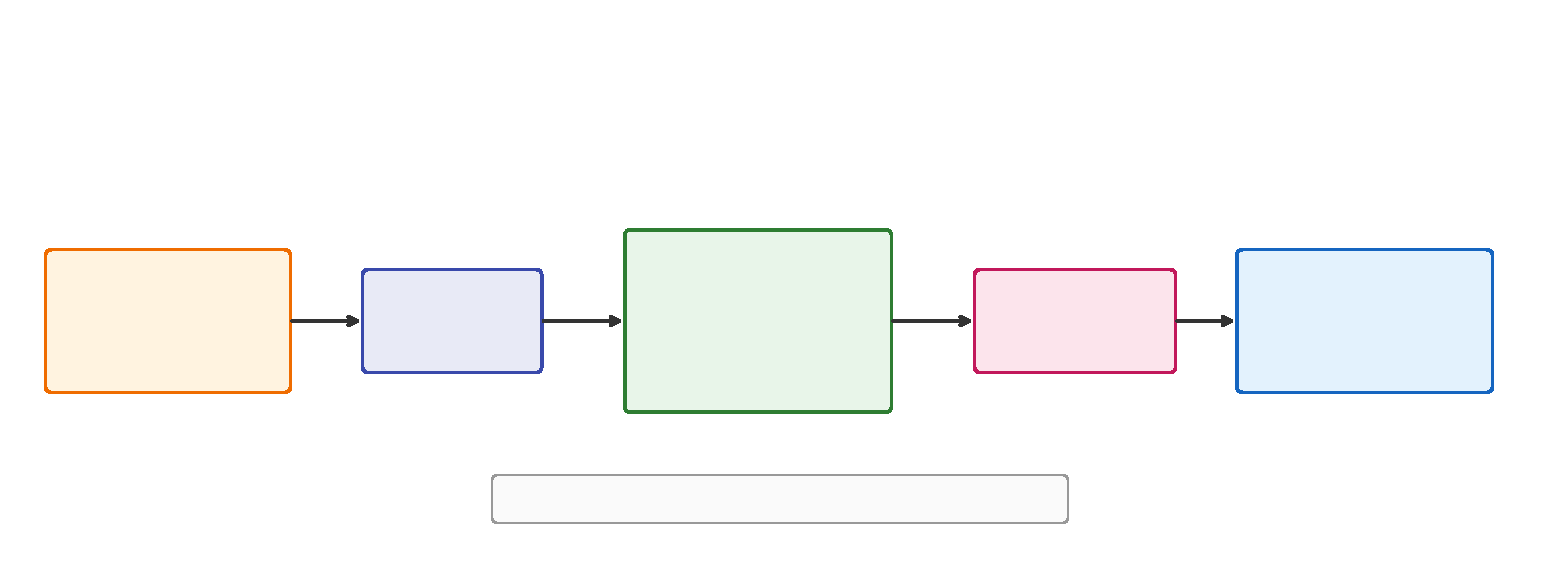
\includegraphics[width=0.95\textwidth]{fig-polarization-projector.pdf}
  \caption{投影仪–场景–相机偏振路径概念草图（非精确工程图）。镜面反射常保偏，漫射趋向退偏；检偏可抑高光，但损失通量。}
  \label{fig:ch05-polar}
\end{figure}

\subsection{部分相干与干涉可见度}
第~\ref{ch:04}~章已写 $I=I_0(1+V\cos\varphi)$。更一般地，$V$ 受振幅比与复相干度共同限制：光源在时空上完全相干时易于高 $V$；完全非相干则经典双光束干涉条纹不出现。部分相干介于二者之间：在有限光程差、有限光源角尺寸内保持可观测条纹 \citep{BornWolf,GoodmanFourierOptics}。

对结构光投影：许多系统使用 LED + 匀光 + 振幅型图案，并不依赖长程干涉；此时「部分相干」更多影响散斑多少与细微对比度。若系统本质是干涉条纹投射或外差干涉，则光源谱宽、瞳孔填充与振动稳定性直接决定 $V$。

\subsection{散斑：高相干遇到粗糙面}

相干光照射光学粗糙表面（高度起伏与 $\wavelength$ 可比）时，各面元散射的复振幅在空间随机干涉，形成颗粒状强度——散斑。散斑统计与瞳孔、波长、表面相关长度有关；对成像而言：
\begin{itemize}
  \item 散斑是乘性、空间相关的「假纹理」，会骗过立体匹配与相位估计；
  \item 增大照明孔径角、降低时间/空间相干、多波长平均、偏振分集或时间积分下的运动模糊，可抑制表观散斑对比度；
  \item 激光投影结构光必须显式管理散斑；LED 通常温和得多。
\end{itemize}

\subsection{投影仪偏振与 LCoS/DMD 直觉}

部分投影器件对偏振敏感：例如某些液晶相关架构需要特定偏振态才能高效调制；DMD（微镜）本身主要是振幅/方向开关，偏振效应来自前后偏光元件与镀膜。工程要点不是背器件手册全文，而是：
\begin{enumerate}
  \item 投影输出是否已接近线偏；
  \item 相机端再加片时，相对方位如何取（平行/正交）；
  \item 加片后通量损失多少、曝光如何补、$\SNR$ 是否掉出相位预算。
\end{enumerate}


\subsection{消光比与「假正交」}

标称交叉偏振若消光比只有 $10^{2}$--$10^{3}$，强镜面叶仍可能漏过并局部饱和。诊断时不要只看「片已正交」：看高光区是否仍顶死直方图。必要时叠中性密度、降投影局部功率，或接受该区失效掩膜。偏振片光谱透过率不平坦时，彩色三通道 $V$ 不一致，会导致依赖颜色编码的结构光出现通道间相位偏差——应用单通道或预先做通道响应校准。

\subsection{空间相干与光源角尺寸}

即使用宽谱 LED，若经小孔或细光纤再照明，空间相干性上升，粗糙面上的散斑对比度仍可能明显。扩散片、积分球匀光、增大有效光源角尺寸，是降空间相干的常用手段。代价包括：投影图案边缘变钝（又一次与 $\MTF$ 交易）、光能利用率下降。口内级小光机里，匀光与散热、体积纠缠在一起，需要在样机阶段用「静态重复扫描残差是否钉住」来验收散斑，而不是只看单帧好看。

\subsection{与辐射度的衔接}

偏振片插入后，式中的有效 $\Phi$ 与像面 $E$ 同步下降。第~\ref{ch:06}~章的 $\SNR$ 预算必须\textbf{在最终偏振配置下}重测；先在无偏振下估好再加片，会系统性乐观。反之，若交叉偏振消除了饱和，有效动态范围变宽，可能使中等灰度区的实际 $\SNR$ 改善——利弊不能只看平均 DN。

\subsection{推导：马吕斯定律从场投影来}

马吕斯定律是电场投影的平方。设入射线偏光电场振幅 $E_0$，偏振方向与检偏器透光轴夹角 $\theta$。理想检偏器只让透光轴方向的分量通过：透射场 $E_0\cos\theta$，强度正比于场振幅平方，故 $I=I_0\cos^2\theta$（式~\eqref{eq:ch05-malus}）。两点前提：入射光完全偏振；检偏器理想，正交方向透射为零。

\textbf{非理想检偏器。} 实际偏振片对正交分量也有微小透射。设透光轴方向强度透射率 $T_\parallel$，正交方向 $T_\perp$，消光比 $\mathrm{ER}=T_\parallel/T_\perp$。则
\[
  I(\theta)=I_0\bigl(T_\parallel\cos^2\theta+T_\perp\sin^2\theta\bigr).
\]
交叉放置（$\theta=90^\circ$）时剩余 $I_0T_\perp=I_0T_\parallel/\mathrm{ER}$。

\textbf{装调角误差。} 即使偏振片理想，交叉角偏离 $90^\circ$ 一个小角 $\epsilon$，剩余透射比为 $\sin^2\epsilon\approx\epsilon^2$。$\epsilon=5^\circ$ 时 $\sin^25^\circ\approx0.0076$，等效消光比只有约 $130$。两种来源同时存在时，等效消光比约为
\[
  \frac{1}{\mathrm{ER}_{\mathrm{eff}}}\approx\frac{1}{\mathrm{ER}}+\epsilon^2 .
\]
这正是「假正交」的定量含义：标称消光比上千的偏振片，装歪几度就只剩一百多。

\subsection{例：交叉偏振能把高光压到多低}

数量级示意。湿润牙面上一块镜面高光，在不加检偏时比周围漫射区亮 $I_s/I_d=50$ 倍。曝光设为让漫射区落在满阱的 $50\%$。
\begin{enumerate}
  \item \textbf{不加检偏}：高光区为满阱的 $25$ 倍，严重饱和；饱和区条纹削顶，相位不可用（第~\ref{ch:06}~章）。
  \item \textbf{加交叉检偏，$\mathrm{ER}_{\mathrm{eff}}=100$}：镜面反射基本保偏，剩余 $50I_d/100=0.5I_d$；漫射光已退偏，检偏后约剩一半，$0.5I_d$。镜面残余与漫射分量相当，高光区约为漫射区的两倍亮（满阱的 $50\%$），不再饱和；但漫射区信号也减半，需要把曝光或投影亮度加倍才能恢复原来的电子数。
  \item \textbf{$\mathrm{ER}_{\mathrm{eff}}=1000$}：剩余镜面 $0.05I_d$，只占漫射信号的十分之一，高光几乎消失。
\end{enumerate}
曝光加倍后，$\mathrm{ER}_{\mathrm{eff}}=100$ 时高光区约为满阱的 $100\%$，刚好处在饱和边缘；$\mathrm{ER}_{\mathrm{eff}}=1000$ 时约为满阱的 $55\%$，安全。由此得到一条可执行的规则：所需等效消光比 $\gtrsim I_s/I_d$ 的数倍。上例中 $\mathrm{ER}_{\mathrm{eff}}$ 至少应在几百，对应装调角误差小于约 $1.8^\circ$（$\epsilon^2<10^{-3}$）。

\subsection{散斑的数量级：颗粒多大、对比多高}

完全发展的散斑（粗糙度远大于波长、照明高度相干）强度服从负指数分布，散斑对比度 $C=\sigma_I/\langle I\rangle=1$。像面上散斑颗粒的典型尺寸由成像孔径决定，量级为
\[
  \sigma_{\mathrm{sp}}\sim\lambda\,N_{F,w},\qquad N_{F,w}=N_F(1+|m|),
\]
与衍射斑同源（数量级关系，具体系数依定义）。若一个像元内包含 $n_s$ 个独立散斑颗粒，或在曝光时间内平均了 $n_s$ 个独立散斑图样，对比度降为 $C\approx1/\sqrt{n_s}$。

例（数量级示意）：$\lambda=650\,\mathrm{nm}$、$N_F=8$、$|m|=0.4$，$\sigma_{\mathrm{sp}}\sim7\,\mu\mathrm{m}$，比 $3\,\mu\mathrm{m}$ 像元还大，单像元几乎不平均，$C$ 接近 $1$。对结构光，散斑相当于一个随位置变化、但不随时间变化的乘性因子乘在条纹上：同一像素在各相移帧中看到的散斑相同，所以它主要改变 $A$ 和 $M$ 的局部值；但散斑在一个像元内不均匀，又随条纹移动而改变加权，残余部分进入相位，形成固定的颗粒状误差。降低它的手段对应 $1/\sqrt{n_s}$ 的两个出口：增大成像孔径（颗粒变小、像元内平均更多，代价是景深）；或让散斑在曝光内变化（振动漫射片、多角度照明、多波长），代价是系统复杂度。改用低相干光源（第~\ref{ch:04}~章相干长度对照表）则从根本上削弱散斑。

\subsection{与投影器件的接口}

第~\ref{ch:07}~章会讨论 DMD 与 LCoS。从本章角度预先记住一点：LCoS 靠偏振调制灰度，投影出的光本身是线偏光，其偏振方向是\emph{固定的}；DMD 不改变偏振，出射光的偏振取决于光源和照明光路。因此，交叉偏振方案的「起偏器」对 LCoS 可能已经内置，只需在相机前加检偏并对准方位；对 DMD 则需要额外起偏，并承受约一半的光损失。

\section{限度}
\label{sec:ch04-limits}

\begin{itemize}
  \item 未引入斯托克斯矢量与缪勒矩阵的完整推演；复杂多层生物组织散射需专门模型。
  \item 「交叉偏振一定改善重建」不成立：若有用信号本身是镜面叶（极光滑金属形貌），抑镜面可能删掉信息。
  \item 散斑抑制与条纹锐度常冲突：过度空间非相干化可能糊掉高频条纹。
  \item 廉价偏振片的漏光与色偏会引入通道相关误差，彩色结构光尤需标定。
\end{itemize}

\section{对象}
\label{sec:ch04-object}

\textbf{高反牙面 / 唾液膜。} 镜面高光使相机局部饱和，条纹 $V$ 在高光区崩溃，相位出现空洞或跳变。交叉偏振常能明显降高光，使漫射分量上的条纹可读；代价是进光变少——需加长曝光或提高增益，前者怕手持运动模糊，后者抬读出噪声。实践：先定偏振方位使高光最暗，再重做曝光使非高光区灰度落在线性段中部。

\textbf{金属器械入镜。} 探针、车针等进入视场时产生强反射与次级照明，污染牙面条纹。偏振有助于压金属高光；仍需算法层做饱和检测与失效标掩膜，光学不能百分百消除。

\textbf{投影仪偏振态。} 若投影已接近线偏，相机检偏方位差 $45^\circ$ 与 $90^\circ$ 的效果完全不同：应用旋转检偏快速扫描，选「高光最小且条纹 $V$ 最大」的折中角，而不是以为「理论上正交」就结束。记录该角为工艺参数，与 $K$、$R,t$ 一并纳入设备配置。

\textbf{散斑诊断。} 激光原型机点云呈颗粒状抖动、静态场景反复扫描噪声图案几乎「钉住」——高度怀疑散斑而非随机读出噪声。对策：扩散片、摆动散射片、多帧平均、换短相干光源；换匹配窗口大小通常治标不治本。


\textbf{偏振方位工艺卡。} 将检偏转台分度，对同一高反样本记录：饱和像素比例、条纹区平均 $V$、平面重复扫描 RMS。选取饱和可控且 RMS 最小的方位写入设备配置，并与温度/清洁周期一并维护。更换偏振片批次后重做该卡。

\section*{本章收束}
偏振改的是哪一路光能进相机；部分相干与散斑改的是假纹理与可见度。高反牙面与金属是对象场上的硬例子：交叉偏振常有效，但必须重做 $\SNR$ 账。下一章把 $\Phi$、$L$、$E$ 与灰度、噪声写清楚。

\section{习题}
\label{sec:ch04-exercises}

\begin{enumerate}
  \item \textbf{（概念）} 马吕斯定律下，$\theta$ 从 $0^\circ$ 转到 $60^\circ$，理想透射强度变为原来的多少？这对 $\SNR$ 意味着什么？
  \item \textbf{（概念）} 为何「图像变暗」不等于「对比度变差」？举一个交叉偏振同时使平均灰度下降、条纹 $V$ 上升的情形。
  \item \textbf{（计算）} 设加检偏后通量变为原来的 $1/4$，光子噪声限下 $\SNR$ 大致如何变？（按 $\SNR\propto\sqrt{N_{\mathrm{ph}}}$ 粗估。）
  \item \textbf{（重建场景）} 湿润牙面高光饱和，交叉偏振后高光消失但整体噪声大、细条纹发灰。给出曝光与条纹频率的调整策略。
  \item \textbf{（重建场景）} 激光结构光静态重复性差、误差图呈固定颗粒。优先怀疑标定漂移还是散斑？如何用实验区分？
  \item \textbf{（综合）} 部分相干光源使真干涉 $V$ 下降，却可能改善散斑。这对「干涉测距」与「投影纹理立体」两种系统的选型启示有何不同？
  \item \textbf{（诊断）} 金属车针进入口内视野导致局部条纹翻转难解。除偏振外，还需要光学或流程上的哪两条措施？
  \item \textbf{（推导）} 写出非理想检偏器且存在装调角误差 $\epsilon$ 时交叉透射率的表达式，并推出 $1/\mathrm{ER}_{\mathrm{eff}}\approx1/\mathrm{ER}+\epsilon^2$ 所需的近似。
  \item \textbf{（计算）} 偏振片标称 $\mathrm{ER}=500$，交叉角误差 $2^\circ$。求 $\mathrm{ER}_{\mathrm{eff}}$。若高光比 $I_s/I_d=80$，按正文规则是否够用？
  \item \textbf{（口扫场景）} 正文高光例中，若改为先降曝光、使高光不饱和，而不加偏振片，漫射区电子数变为原来的多少？按 $\SNR\propto\sqrt{N_e}$，相位噪声变为多少倍？与交叉偏振方案比较。
  \item \textbf{（计算）} 激光投影 $\lambda=520\,\mathrm{nm}$，$N_F=4$，$|m|=0.4$，像元 $2\,\mu\mathrm{m}$。估算散斑颗粒尺寸；若用振动漫射片在每帧曝光内平均 $25$ 个独立图样，散斑对比度变为多少？
  \item \textbf{（医学重建）} 皮肤表面的镜面反射较弱、次表面散射较强。交叉偏振在这里的主要作用与牙面有何不同？（提示：次表面散射光的偏振状态。）
\end{enumerate}

\section{习题讲解}
\label{sec:ch04-solutions}

\begin{enumerate}
  \item $\cos^{2}60^\circ=1/4$，强度降为 $1/4$。若读出噪声不可忽略，$\SNR$ 往往掉得比 $2$ 倍（$\sqrt{4}$）更狠；需重估曝光。
  \item 对比度/可见度看的是调制相对均值。交叉偏振去掉饱和高光后，条纹区可能从「削顶失真」恢复为高 $V$，尽管平均 DN 更低。
  \item $N_{\mathrm{ph}}\to N_{\mathrm{ph}}/4$，$\SNR\to\SNR/2$（纯泊松）。若还有固定读出噪声，下降更明显。
  \item 适当加长曝光或提高投影亮度恢复电子数；必要时略降条纹频率以适配 $\MTF$；保持检偏方位。避免只靠数字增益。
  \item 优先散斑：误差空间图案在重复扫描中高度相似。标定漂移常表现为缓慢系统性弯曲或尺度变。区分：关激光换 LED/加扩散片看颗粒是否消；或微扰照明角度看散斑是否重排而几何标定不变。
  \item 干涉测距依赖高 $V$ 与稳定相干 → 要管谱宽与振动。投影纹理立体更怕散斑假纹理 → 可牺牲相干换平滑。同一「部分相干」旋钮，两种系统拧的方向相反。
  \item 例：遮挡/避开金属进入光路的操作规范；饱和与高梯度区失效掩膜；局部降曝光或分次扫描。偏振是手段之一，不是唯一。
  \item 设入射与透光轴夹 $90^\circ-\epsilon$：$I/I_0=T_\parallel\sin^2\epsilon+T_\perp\cos^2\epsilon$。除以 $T_\parallel$ 得 $1/\mathrm{ER}_{\mathrm{eff}}=\sin^2\epsilon+\cos^2\epsilon/\mathrm{ER}$；小角下 $\sin^2\epsilon\approx\epsilon^2$、$\cos^2\epsilon\approx1$，即得。
  \item $\epsilon=2^\circ=0.0349\,\mathrm{rad}$，$\epsilon^2\approx1.22\times10^{-3}$；$1/\mathrm{ER}_{\mathrm{eff}}\approx0.002+0.00122=0.00322$，$\mathrm{ER}_{\mathrm{eff}}\approx310$。$I_s/I_d=80$ 时剩余镜面约 $80/310\approx0.26I_d$，相对检偏后漫射 $0.5I_d$ 约一半；曝光加倍后高光区约为满阱的 $76\%$，不饱和但余量不大。按「数倍于 $I_s/I_d$」的规则属勉强够用。
  \item 高光原为满阱 $25$ 倍，要压到满阱以下，曝光须降到约 $1/25$，漫射区电子数也降到 $1/25$；$\SNR$ 降为 $1/5$，相位噪声增为约 $5$ 倍。交叉偏振方案只损失一半信号（曝光加倍可补回），明显更优。另一种做法是多曝光融合，但需要更多帧。
  \item $\sigma_{\mathrm{sp}}\sim0.52\times4\times1.4\approx2.9\,\mu\mathrm{m}$，略大于像元。平均 $25$ 个独立图样后 $C\approx1/5=0.2$。
  \item 次表面散射光多次散射后基本退偏，交叉偏振会保留它、去掉表面镜面反射。牙面上交叉偏振主要用来去高光；皮肤上它反而突出了次表面散射成分（图像看起来更「均匀、深」），会加剧条纹调制度下降和深度偏置。若目标是表面几何，平行偏振（保留表面反射）有时更有利，需要实验比较。
\end{enumerate}

\chapter{投影光学与结构光}
\label{ch:06}

\section{效果}
\label{sec:ch06-effect}

读完本章，你应能：
\begin{enumerate}
  \item 把投影仪看作「倒装的相机」，说明其光路、景深与畸变如何进入结构光几何；
  \item 写出正弦条纹模型与 $N$ 步相移求相位 $\varphi$ 的公式，并给出调制度、$\SNR$ 与相位噪声的关系；
  \item 用时间相位展开、多频外差与格雷码的直觉解释「包裹相位如何变成绝对相位」，以及各自的失效方式；
  \item 叙述从绝对相位到深度 $(X,Y,Z)$ 的标定链；
  \item 说明 DMD 与 LCoS 的调制概念：二值调制、离焦成正弦、伽马非线性、帧同步；
  \item 诊断口内结构光中的高反、次表面散射与运动伪影。
\end{enumerate}

\section{原理}
\label{sec:ch06-principle}

\subsection{投影仪：倒装的相机}

投影仪由光源、匀光、空间光调制器（DMD 或 LCoS 等）与投影镜头组成。几何上，它与相机互为对偶：相机把空间射线映到像素 $(u,v)$；投影仪把调制器像素 $(u_p,v_p)$ 映为空间射线。因此投影仪同样有内参 $K_p$、畸变与外参，第~\ref{ch:02}~章的模型可原样搬用，只是「像面」换成调制器平面。

投影镜头的景深同样有限。条纹投到工作距范围之外时，投影侧离焦先把条纹模糊，相机侧离焦再模糊一次；两次 $\PSF$ 的卷积共同决定相机所见调制度。口内设备常让投影与相机共用或靠近同一工作距，并选较小相对孔径以换取景深 $Z_d$，代价是光通量（第~\ref{ch:05}~章）。

\subsection{正弦条纹模型}

投影仪沿一个方向（设为 $u_p$）投出周期为 $P$ 像素的正弦条纹。物体表面反射后，相机像素 $(u,v)$ 处的第 $k$ 帧灰度可写作
\begin{equation}
  I_k(u,v)=A(u,v)+M(u,v)\cos\!\bigl(\varphi(u,v)+\delta_k\bigr),\qquad k=0,\dots,N-1,
  \label{eq:ch06-fringe}
\end{equation}
其中 $A$ 为背景（含环境光与平均反射），$M$ 为调制幅度，$\delta_k$ 为第 $k$ 帧的已知相移，$\varphi$ 为待求相位。$\varphi$ 编码了「该相机像素看到的是投影仪哪一列」：$u_p=\dfrac{P}{2\pi}\varphi$。这里的强度沿用相对强度 $I$，前提是相机工作在线性区且曝光锁定（第~\ref{ch:05}~章）。

相机所见的调制度（条纹对比度）记为 $V=M/A$，与第~\ref{ch:03}~章的可见度是同一个量；投影端（调制器上）的调制度记为 $V_0$。离焦、次表面散射、环境光都会降低 $V$。

\subsection{$N$ 步相移}

取等间隔相移 $\delta_k=2\pi k/N$（$N\ge3$）。最小二乘解为
\begin{equation}
  \varphi_w=\operatorname{atan2}\Bigl(-\sum_{k}I_k\sin\delta_k,\ \sum_{k}I_k\cos\delta_k\Bigr),
  \label{eq:ch06-nstep}
\end{equation}
\begin{equation}
  M=\frac{2}{N}\sqrt{\Bigl(\sum_k I_k\sin\delta_k\Bigr)^2+\Bigl(\sum_k I_k\cos\delta_k\Bigr)^2},
  \qquad
  A=\frac{1}{N}\sum_k I_k.
  \label{eq:ch06-AM}
\end{equation}
四步（$N=4$）时简化为
\[
  \varphi_w=\operatorname{atan2}(I_3-I_1,\ I_0-I_2).
\]
所得 $\varphi_w$ 落在 $(-\pi,\pi]$，称为包裹相位（图~\ref{fig:ch06-fringe}）。

\textbf{相位噪声。} 若每帧灰度噪声标准差为 $\sigma_I$（加性、独立），相位标准差约为
\begin{equation}
  \sigma_{\varphi}\approx\sqrt{\frac{2}{N}}\,\frac{\sigma_I}{M}.
  \label{eq:ch06-phase-noise}
\end{equation}
即相位精度正比于「调制幅度对噪声」的比，而不是「平均亮度对噪声」。$M$ 小而 $A$ 大（环境光强、散射严重）时，光子噪声随 $A$ 增长而 $M$ 不长，相位反而更差。这是结构光的 $\SNR$ 应定义在调制项上的原因。增大 $N$ 以 $\sqrt{N}$ 降噪，但需要更多帧，对运动更敏感。

$N$ 步相移还有一个好处：若相机或投影存在伽马非线性，谐波会引入周期性相位误差；$N$ 越大，越高阶的谐波才会混叠进相位，因此误差越小。

\begin{figure}[htbp]
  \centering
  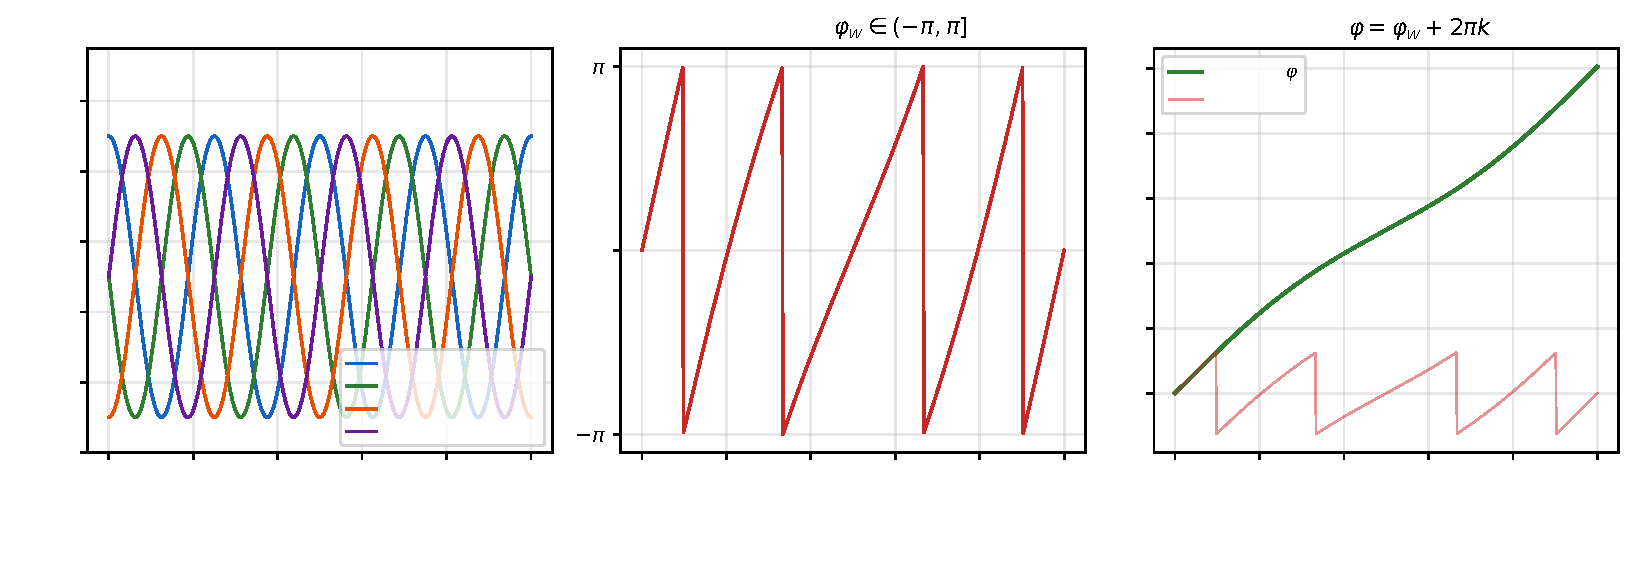
\includegraphics[width=0.98\textwidth]{fig-fringe-phase.pdf}
  \caption{四步相移条纹截面、包裹相位与展开相位的概念草图（非精确工程图）。}
  \label{fig:ch06-fringe}
\end{figure}

\subsection{相位展开}

包裹相位只给出「在一个条纹周期内的位置」，还需确定整数级次 $k$：$\varphi=\varphi_w+2\pi k$。两类思路：

\textbf{空间展开。} 沿图像路径累加相邻像素的相位差，假设相邻像素差不超过 $\pi$。在连续光滑表面有效；遇到遮挡、陡坡、孤立区域（牙间隙、器械边缘）时会把错误传播开来。质量引导、最小范数等方法改进了鲁棒性，系统论述见 \citet{GhigliaPritt1998}。

\textbf{时间展开。} 每个像素独立地用额外图案确定 $k$，不依赖邻域，因此对不连续表面更稳。常见三种：
\begin{itemize}
  \item \textbf{多频（外差）}：投两个或多个周期 $P_1<P_2$ 的条纹，其相位差相当于等效长周期 $P_{\mathrm{eq}}=P_1P_2/(P_2-P_1)$。等效周期覆盖整个视场时，即可逐级确定高频条纹的级次。代价是噪声在逐级推导中被放大 $P_{\mathrm{eq}}/P_1$ 倍，频率比不能选得过大。
  \item \textbf{格雷码}：投 $m$ 幅二值图案，给每个条纹周期编号 $0,\dots,2^m-1$。格雷码相邻编号只差一位，边界上误判最多错一级。弱点是黑白边界处被模糊后易判错，常出现「级次跳变一个周期」的线状误差，需要与包裹相位边界对齐校正。
  \item \textbf{相位编码 / 其他}：把级次编码在额外的相位图中，原理相近。
\end{itemize}
共同点：高频条纹负责精度，低频或编码负责唯一性。设计时先让最高频条纹在工作距内仍有足够 $M$（第~\ref{ch:03}~章的通带），再选最少的辅助图案保证展开正确。

\subsection{从相位到深度：标定链}

绝对相位 $\varphi$ 给出投影仪列坐标 $u_p$。与相机像素 $(u,v)$ 一起，就有一对对应：相机射线与投影仪的一张「光平面」（单方向条纹时是平面，而非射线）。三角求交即得 $(X,Y,Z)$。所需参数：
\begin{enumerate}
  \item 相机内参 $K$ 与畸变；
  \item 投影仪内参 $K_p$ 与畸变（通常借助相机「替投影仪看」标定板：投影仪通过相位反算标定板角点的 $(u_p,v_p)$）；
  \item 两者相对外参 $R,t$。
\end{enumerate}
另一种做法是\textbf{相位–高度查表}：在若干已知高度的平面上记录每像素的相位，拟合 $Z=g_{uv}(\varphi)$ 多项式。查表绕开显式模型，对投影畸变不敏感，但只在标定过的深度范围内可靠，外推会出错。

两种方法都要求：标定时与工作时的曝光、对焦、伽马处理、投影亮度完全一致；任何改变都会使 $\varphi$ 到 $Z$ 的映射漂移。

\subsection{DMD 与 LCoS：调制概念}

\textbf{DMD（数字微镜器件）} 由大量可在两种倾角间翻转的微镜组成。「开」镜把光反射进投影镜头，「关」镜反射到吸收器。单个微镜只能二值；灰度靠在一帧内按比特面控制开关时间（脉宽调制）。这带来两个工程后果：
\begin{itemize}
  \item 相机曝光若不是比特周期的整数倍，或未与投影帧同步，会截取到不完整的比特序列，灰度出错，表现为条纹「跳灰度」或帧间闪烁；
  \item 灰度正弦需要多个比特面，帧率下降。
\end{itemize}

\textbf{二值离焦法}：直接投二值方波条纹，让投影镜头适度离焦，方波高次谐波被 $\MTF$ 衰减，到达物体时近似正弦（图~\ref{fig:ch06-dmd}）。优点：一个比特面一帧，可上千赫兹，并且没有伽马问题。缺点：近似正弦的程度依赖离焦量，即依赖深度；残余谐波造成周期性相位误差。

\textbf{LCoS（硅基液晶）} 通过液晶对偏振态的调制实现连续灰度，需要偏振光照明与检偏（第~\ref{ch:04}~章），响应较慢，有灰度–电压非线性。

\textbf{伽马。} 投影仪与相机的灰度响应常非线性，投入的「正弦」实际变成含谐波的周期曲线，导致相位误差呈条纹周期的 $N$ 倍频波纹。对策：标定伽马曲线并预失真；或增加相移步数；或使用二值离焦。

\begin{figure}[htbp]
  \centering
  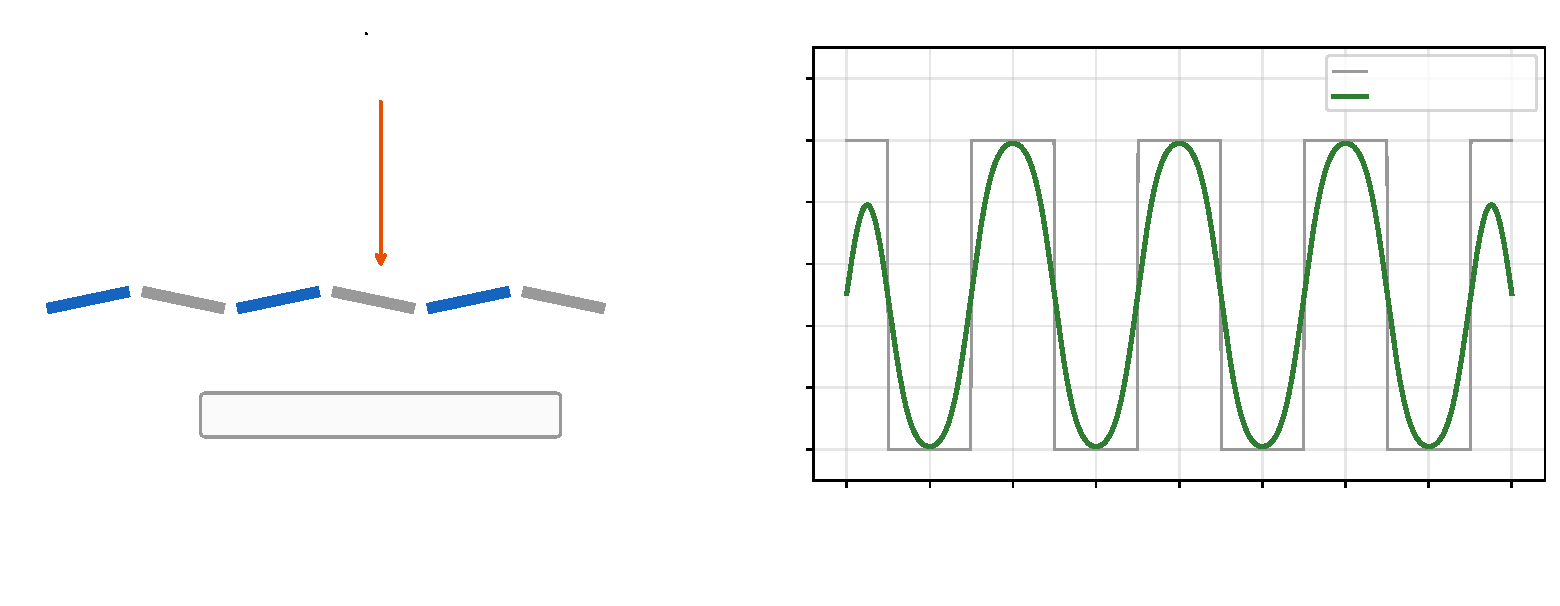
\includegraphics[width=0.95\textwidth]{fig-dmd-concept.pdf}
  \caption{DMD 微镜二值开关与二值条纹经离焦近似为正弦的概念草图（非精确工程图）。}
  \label{fig:ch06-dmd}
\end{figure}

\section{限度}
\label{sec:ch06-limits}

\begin{itemize}
  \item 式~\eqref{eq:ch06-fringe} 假设每像素只接收来自投影仪一个位置的直接反射。次表面散射与互反射违反该假设，属于模型误差，不是噪声。
  \item 式~\eqref{eq:ch06-phase-noise} 假设加性独立噪声与静止物体；运动与非线性误差需要另外计算。
  \item 多频与格雷码展开都假设辅助图案在工作距内可辨；景深外首先失效的往往是展开，而不是包裹相位本身。
  \item 相位–高度查表只对标定范围内深度有效。
  \item 本章不涉及单帧方法（傅里叶变换轮廓术、彩色编码、学习方法）的完整推导；它们以空间带宽或颜色换时间，仍受同样的光学限制。
\end{itemize}

\section{对象}
\label{sec:ch06-object}

\textbf{口内结构光。} 工作距约十余毫米，景深仅数毫米，探头手持移动。常见折中：中高频条纹 + 少帧相移 + 时间展开，配合高帧率投影与全局快门相机。每多一帧，运动伪影风险就增加一份；每少一帧，相位噪声与伽马误差就增加一份。

\textbf{高反（釉质湿润面、金属修复体）。} 高光处相机饱和，式~\eqref{eq:ch06-fringe} 削顶，相位错误且 $M$ 计算值异常。诊断：检查 $I_k$ 是否触顶；用 $M$ 与 $A$ 做质量图并掩膜。对策：交叉偏振、多曝光合成（锁定每档曝光，不用自动曝光）、喷粉（临床上逐渐被避免）。

\textbf{次表面散射（牙本质、牙龈、半透明修复材料）。} 光进入材料后在内部扩散再射出，相当于条纹被一个空间核模糊并平移。结果：调制度 $M$ 下降、相位偏移，深度出现系统性的「下沉」或「平滑」。中低频条纹下，散射核宽度小于周期，散射光仍带着被平移的条纹，造成相位偏置；当条纹周期明显短于散射核宽度时，散射光被平均成近似常数，进入 $A$ 而不再偏置 $\varphi$，代价是 $M$ 降低。对策因此是：在 $M$ 仍够用的前提下提高条纹频率；短波长（蓝光）穿透更浅，常用于口内。

\textbf{运动伪影。} $N$ 帧之间物体移动 $\Delta u$ 像素，相当于每帧的 $\varphi$ 不同，求解得到的相位有与条纹同周期的波纹误差。诊断：静止模型上误差消失；误差随移动速度增大。对策：缩短总采集时间（提高投影帧率、减少帧数）、运动补偿、或用对运动不敏感的编码顺序。

\section*{本章收束}
结构光把「投影仪哪一列照到这里」编码为相位 $\varphi$。相移决定相位精度，展开决定唯一性，标定决定相位到深度的映射。DMD 与 LCoS 的调制方式决定伽马、同步与帧率。对象场景中的误差大多可归入：调制度不足、模型假设被违背（散射、饱和）、帧间不一致（运动、曝光）。下一章讨论三角测量本身如何放大这些误差。

\section{习题}
\label{sec:ch06-exercises}

\begin{enumerate}
  \item \textbf{（计算）} 四步相移得到 $I_0=180,\ I_1=100,\ I_2=60,\ I_3=140$。求包裹相位 $\varphi_w$、$A$、$M$ 与调制度 $M/A$。
  \item \textbf{（计算）} 三步与六步相移，若 $\sigma_I/M$ 相同，相位标准差之比是多少？六步的代价是什么？
  \item \textbf{（计算）} 两组条纹周期 $P_1=16$ 像素、$P_2=18$ 像素。求等效周期 $P_{\mathrm{eq}}$。若投影仪宽 $912$ 像素，等效周期能否覆盖全宽？噪声放大倍数约为多少？
  \item \textbf{（重建场景）} 某口内扫描点云在牙龈与半透明修复体上比釉质「低」约几十微米，且条纹频率提高后差异减小。解释原因。
  \item \textbf{（重建场景）} 点云上出现沿条纹方向、间距恰为一个条纹周期深度的线状台阶。最可能是哪一步出错？如何确认？
  \item \textbf{（重建场景）} 相位误差图出现频率为条纹频率 $4$ 倍的规则波纹（四步相移）。可能原因是什么？给出两种对策。
  \item \textbf{（设计）} DMD 投影帧率 $1000$ 帧/秒（二值），相机全局快门。设计一个「二值离焦 + 时间展开」的采集序列，估计总时长，并说明手持速度 $20\,\mathrm{mm/s}$ 时的运动量。
\end{enumerate}

\section{习题讲解}
\label{sec:ch06-solutions}

\begin{enumerate}
  \item $\varphi_w=\operatorname{atan2}(I_3-I_1,\,I_0-I_2)=\operatorname{atan2}(40,120)\approx0.32\,\mathrm{rad}$。$A=(180+100+60+140)/4=120$。$M=\tfrac12\sqrt{40^2+120^2}\approx63.2$。调制度 $M/A\approx0.53$。
  \item $\sigma_\varphi\propto\sqrt{2/N}$，三步比六步为 $\sqrt{6/3}=\sqrt2\approx1.41$。六步需双倍时间，运动更敏感，帧率更低。
  \item $P_{\mathrm{eq}}=16\times18/(18-16)=144$ 像素，不足以覆盖 $912$ 像素，需要第三个频率或格雷码辅助。噪声放大约 $P_{\mathrm{eq}}/P_1=9$ 倍，因此级次判定要求低频相位噪声小于约 $\pi/9$。
  \item 次表面散射：光在半透明材料内扩散，条纹被模糊并偏移，相位偏置使深度系统性偏差。提高条纹频率使散射成分更接近常数背景，偏置减小。
  \item 相位展开级次错一级（格雷码边界误判或多频级次误判）。确认：在包裹相位图上看台阶是否位于 $\pm\pi$ 跳变处；检查格雷码解码在边界上是否与包裹相位不同步。
  \item 伽马非线性（投影或相机），也可能是 DMD 未同步导致的灰度误差。对策：伽马标定与预失真；增加相移步数；改二值离焦；检查帧同步。
  \item 例：$3$ 幅格雷码或 $2$ 组低频 + $4$ 步高频相移，约 $7$--$12$ 帧，$7$--$12\,\mathrm{ms}$。移动 $0.14$--$0.24\,\mathrm{mm}$，相对于数十微米的精度目标很大，需要缩短序列或做运动补偿。
\end{enumerate}

\chapter{立体视觉与三角测量的光学限度}
\label{ch:07}

\section{效果}
\label{sec:ch07-effect}

读完本章，你应能：
\begin{enumerate}
  \item 由基线 $B$、焦距 $f_x$ 与视差写出三角测量关系，并推导误差放大 $\delta Z\sim Z^2\delta d/(Bf_x)$；
  \item 说明交会角如何同时影响精度、遮挡与匹配难度；
  \item 解释景深与基线之间的冲突，以及它为何常常决定紧凑探头的上限；
  \item 把标定误差（内参、外参、畸变）沿三角测量传播到 $(X,Y,Z)$；
  \item 比较相机–投影仪对与双相机立体，并为口内扫描仪做一份精度预算。
\end{enumerate}

\section{原理}
\label{sec:ch07-principle}

\subsection{投影与三角测量}

沿用第~\ref{ch:02}~章的针孔模型：
\begin{equation}
  s\begin{pmatrix}u\\v\\1\end{pmatrix}=K\,[R\mid t]\begin{pmatrix}X\\Y\\Z\\1\end{pmatrix},
  \label{eq:ch07-proj}
\end{equation}
$s$ 为齐次尺度。两个视图（两台相机，或相机与投影仪）各给出一条射线，射线的交点即为物点。实际中两射线因噪声不相交，常取最小化重投影误差的点 \citep{HartleyZisserman2004}。

\textbf{平行校正的标准形。} 两个相机光轴平行、基线 $B$ 沿 $X$ 方向、焦距同为 $f_x$（像素单位，$f_x=f/p$，$f$ 为毫米焦距、$p$ 为像元间距）。视差 $d=u_1-u_2$，则
\begin{equation}
  Z=\frac{Bf_x}{d}.
  \label{eq:ch07-disparity}
\end{equation}
对 $d$ 求导：
\begin{equation}
  \delta Z=\frac{Bf_x}{d^2}\,\delta d=\frac{Z^2}{Bf_x}\,\delta d.
  \label{eq:ch07-error}
\end{equation}
这就是第~\ref{ch:02}~章预告的误差放大。记号约定：$\delta u$ 表示单个视图中的像面定位误差，$\delta d$ 表示视差误差。双相机且两侧误差独立同分布时 $\delta d=\sqrt2\,\delta u$；相机–投影仪对中投影侧坐标由相位给出，$\delta d$ 即相位误差折算到相机像素的等效值。第~\ref{ch:02}~章的 $\delta u$ 估计在这里应理解为 $\delta d$ 的来源。三个结论：深度误差随 $Z^2$ 增长；与基线、焦距成反比；与匹配精度 $\delta d$（亚像素级）成正比（图~\ref{fig:ch07-tri}）。

对结构光，$\delta d$ 来自第~\ref{ch:06}~章的相位噪声：$\delta u_p=\dfrac{P}{2\pi}\sigma_\varphi$，再按投影仪与相机的焦距之比折算。于是「条纹周期 $P$ 越短、调制度越高、$\SNR$ 越高」直接转化为更小的 $\delta Z$。

\textbf{横向误差。} $X=Zu'/f_x$（$u'$ 为相对主点的坐标），故 $\delta X\approx (Z/f_x)\delta u+(X/Z)\delta Z$。横向误差主要随 $Z$ 线性增长，通常小于深度误差，除非视场边缘 $X/Z$ 较大。

\begin{figure}[htbp]
  \centering
  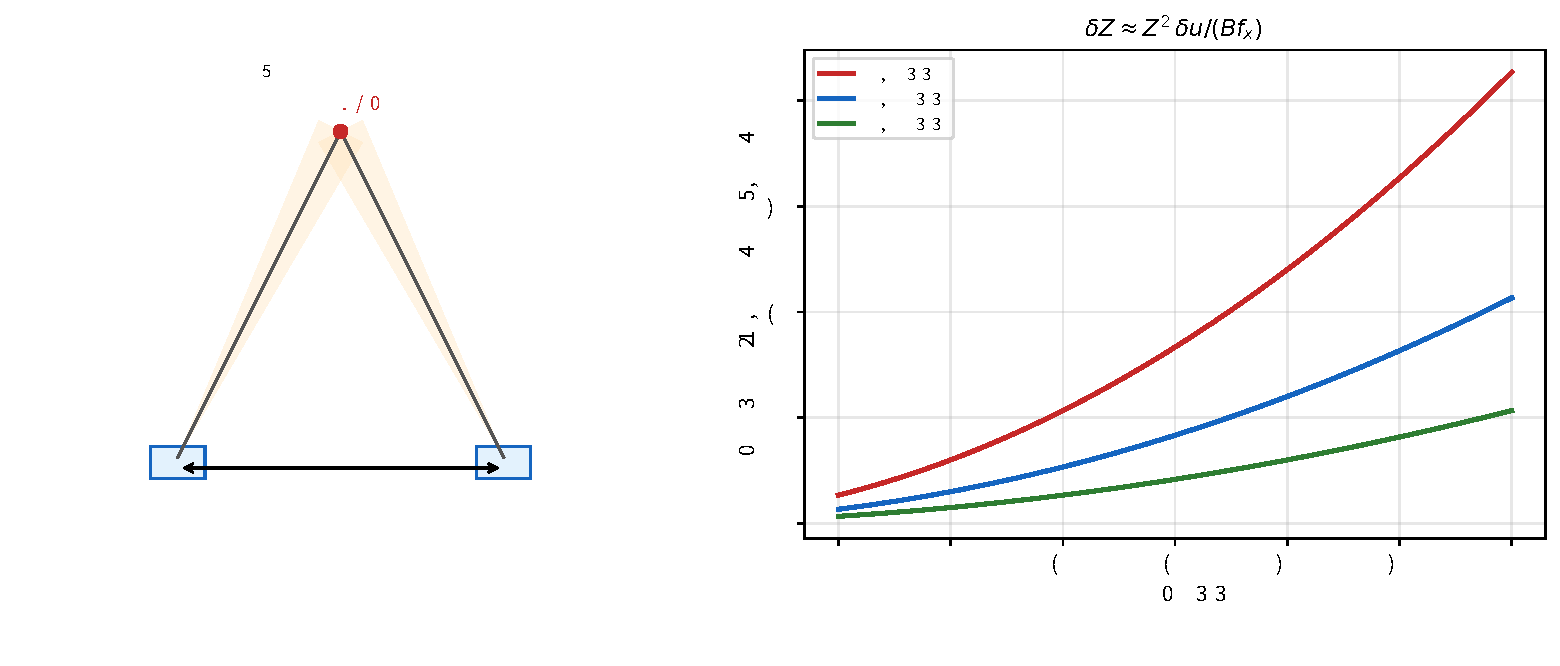
\includegraphics[width=0.98\textwidth]{fig-stereo-triangulation.pdf}
  \caption{三角测量、交会角与误差随工作距和基线变化的概念草图（非精确工程图）。}
  \label{fig:ch07-tri}
\end{figure}

\subsection{匹配精度从哪里来}

式~\eqref{eq:ch07-error} 中的 $\delta d$ 不是一个固定常数，而是光学与信号处理共同决定的量。对被动立体，$\delta d$ 取决于局部纹理的对比度与 $\SNR$：纹理越弱、模糊越重，相关峰越宽，亚像素定位越差。对结构光，$\delta d$ 取决于相位噪声与条纹周期：周期 $P$ 越短，相位误差折算成的像素误差越小，但周期不能短于光学系统在整个景深内能够传递的空间频率，否则调制度 $M$ 先崩溃（第~\ref{ch:03}~章的 $\MTF$ 讨论）。因此，「提高精度」的三条路径——增大基线、增大焦距、降低匹配误差——各自都撞上一个光学墙：基线撞上体积与遮挡，焦距撞上视场与景深，匹配误差撞上 $\MTF$ 与光子噪声。

还应区分相机像素与投影仪像素。投影仪分辨率往往低于相机，但相位编码是连续量，投影仪像素的离散性只在二值或伽马失真时显现；真正限制精度的通常是相机一侧的 $\SNR$ 与模糊。若投影侧离焦严重，条纹在物面已被抹平，相机再清晰也无济于事。设计时可以把两侧的 $\PSF$ 投影到物面上比较，较宽的一侧就是匹配精度的瓶颈。

\subsection{交会角}

非平行配置下，用交会角 $\theta$（两射线在物点的夹角）更直观。若每条射线的角度误差为 $\delta\alpha\approx\delta u/f_x$，则沿二者平分线方向的深度误差约为
\begin{equation}
  \delta Z\approx\frac{Z\,\delta\alpha}{2\sin(\theta/2)},
  \label{eq:ch07-angle}
\end{equation}
小角度时 $2\sin(\theta/2)\approx\theta\approx B/Z$，回到式~\eqref{eq:ch07-error}（两视图噪声独立时再乘约 $\sqrt2$ 的常数因子）。交会角越大，精度越好；但同时：
\begin{itemize}
  \item 两视图看到的表面外观差异更大（透视变形、镜面反射位置不同），匹配更难；
  \item 遮挡与阴影增多；
  \item 对结构光，投影条纹在斜面上压缩或拉伸更明显。
\end{itemize}
经验上交会角常取 $10^\circ$--$30^\circ$，具体取决于场景几何。

\subsection{遮挡与阴影}

三角测量要求物点同时被两个视图看见。双相机系统中，一台相机能看到、另一台看不到的区域称为\textbf{遮挡}。相机–投影仪系统中，投影仪照不到的区域称为\textbf{阴影}，相机看不到的区域同样是遮挡。两者都会导致缺失数据，并且基线越大、表面越陡（牙间隙、龈沟、深窝洞）越严重。

处理方式：多视角拼接（手持扫描不断换角度）；多投影器或多相机；接受部分缺失，由后续融合补洞。其中「缺失」是可诊断的；更危险的是边界处的\textbf{混合像素}：一个像素同时包含前景与背景，或在阴影边缘接收了部分条纹，产生「飞点」。

\subsection{景深与基线的冲突}

精度希望 $B$ 大、$f_x$ 大、$Z$ 小。但：
\begin{itemize}
  \item 景深 $Z_d$ 随相对孔径减小而增大，随焦距增大、工作距减小而迅速缩小（第~\ref{ch:01}~章）。$f_x$ 大且 $Z$ 小意味着景深浅。
  \item 基线 $B$ 大意味着交会角大，同一深度范围内物点在两视图中横移更多，所需的共同视场与有效景深范围被压缩。
  \item 为扩展景深而缩小孔径，会降低通光量与衍射极限分辨（第~\ref{ch:03}~章、第~\ref{ch:05}~章），使 $\delta u$ 变大。
\end{itemize}
因此存在一个最优区间：在给定探头尺寸、工作距与深度范围下，$B$ 与孔径被同时约束。紧凑探头（如口内）往往不是被三角公式限制，而是被「探头头部放不下更大的基线」与「景深要覆盖整颗牙」两条硬约束限制。

\subsection{标定误差传播}

三角测量的输入除了 $(u,v)$ 外，还有 $K$、畸变、$R$、$t$。常见误差：
\begin{itemize}
  \item \textbf{基线长度误差} $\delta B$：由式~\eqref{eq:ch07-disparity}，$\delta Z/Z=\delta B/B$，产生整体尺度误差；对比测量长度（如牙弓跨度）时出现等比例偏差。
  \item \textbf{焦距误差} $\delta f_x$：同样是尺度误差 $\delta Z/Z=\delta f_x/f_x$。
  \item \textbf{主点 / 旋转误差}：等价于视差上的常数偏置 $\Delta d$，$\delta Z\approx Z^2\Delta d/(Bf_x)$，随深度非线性变化，把平面扭成曲面。
  \item \textbf{残余畸变}：在视场边缘产生空间相关的深度误差，常表现为平面重建成「碗形」或「马鞍形」。
\end{itemize}
标定本身使用 \citet{Zhang2000Calibration} 一类方法，其精度受标定板制造误差、角点检测精度、姿态多样性限制。关键原则：标定的深度范围与姿态应覆盖工作范围，否则外推误差会以 $Z^2$ 方式出现。

\subsection{相机–投影仪对与双相机立体}

\begin{itemize}
  \item \textbf{双相机立体}：被动或主动照明。被动立体依赖表面纹理，在光滑釉质上难以匹配；加上随机散斑投影可提供纹理，但不必标定投影仪。对应是二维搜索（沿极线一维）。
  \item \textbf{相机–投影仪对}：对应由相位直接给出，几乎没有匹配歧义；但需要标定投影仪，且投影仪的畸变、伽马、热漂移都进入误差。
  \item \textbf{双相机 + 投影条纹}：用相位作为「纹理」在两相机间匹配，投影仪不进入几何模型，只需相位稳定。代价是两个相机都要看到、多一台相机的体积与成本，以及阴影与遮挡的并集。
\end{itemize}
选型时考虑：哪个器件的几何最稳定（相机通常比投影仪稳定）；体积；遮挡模式；匹配歧义。

\subsection{推导：深度误差的一阶与二阶项}

由相似三角形，平行双目中 $Z=f_xB/d$（式~\eqref{eq:ch07-disparity}）。对 $d$ 求导：
\[
  \frac{\partial Z}{\partial d}=-\frac{f_xB}{d^2}=-\frac{Z^2}{f_xB},
\]
取绝对值即一阶误差 $\delta Z=Z^2\delta d/(f_xB)$。适用条件：$\delta d\ll d$。

\textbf{二阶偏置。} $Z$ 是 $d$ 的凸函数，零均值的视差噪声会让 $Z$ 的期望偏大。设 $d$ 的噪声 $e$ 均值零、方差 $\sigma_d^2$，展开
\[
  \frac{1}{d+e}=\frac1d\Bigl(1-\frac ed+\frac{e^2}{d^2}-\cdots\Bigr),\qquad
  \mathbb E[Z]\approx Z\Bigl(1+\frac{\sigma_d^2}{d^2}\Bigr).
\]
偏置 $Z\sigma_d^2/d^2$。第~\ref{ch:00}~章的几何中 $f_xB=12000\,\mathrm{mm}\cdot$像素、$Z=15\,\mathrm{mm}$，$d=800$ 像素；$\sigma_d=0.051$ 像素时偏置约 $15\times(6\times10^{-5})^2\,\mathrm{mm}$，完全可忽略。但远距被动立体常见 $d\approx20$ 像素、$\sigma_d\approx1$ 像素，偏置为 $Z$ 的 $0.25\%$，在 $Z=4\,\mathrm{m}$ 时约 $1\,\mathrm{cm}$，且平均多帧也不会消失。这提醒我们：对深度取平均之前，最好先对视差取平均。

\subsection{推导：相机射线与投影光平面求交}

结构光常用「相机 + 投影仪」而非两台相机。相位确定投影仪的一列，即空间中一张光平面 $\boldsymbol n^\top\boldsymbol X=h$（在相机坐标系中表示，$\boldsymbol n$ 与 $h$ 由标定给出）。相机像素的归一化射线 $\boldsymbol X=t\,\tilde{\boldsymbol x}$，$\tilde{\boldsymbol x}=(x,y,1)^\top$。代入平面方程：
\[
  t=\frac{h}{\boldsymbol n^\top\tilde{\boldsymbol x}},\qquad Z=t .
\]
每像素只需一次点积与一次除法，适合 GPU 逐像素计算。条件性：当 $\boldsymbol n^\top\tilde{\boldsymbol x}\to0$，射线几乎平行于光平面，$Z$ 对相位与标定误差极端敏感——这正是交会角过小的情形。对平面法向的小误差 $\delta\boldsymbol n$，
\[
  \frac{\delta Z}{Z}\approx-\frac{\delta\boldsymbol n^\top\tilde{\boldsymbol x}}{\boldsymbol n^\top\tilde{\boldsymbol x}},
\]
分母越小，放大越大。实现中应对 $|\boldsymbol n^\top\tilde{\boldsymbol x}|$ 设下限，低于下限的像素直接标为无效，而不是输出一个巨大的深度。

\subsection{例：一张完整的深度误差预算}

把前面各章算过的数放到同一几何（第~\ref{ch:00}~章：$Z=15\,\mathrm{mm}$，$f_xB=12000\,\mathrm{mm}\cdot$像素，$P=16$ 像素，四步相移）下。随机项可按平方和合成；系统项单独列出，因为它们在空间上相关，不随平均下降。数量级示意：

\begin{center}
\small
\begin{tabular}{llll}
  \hline
  来源 & 相位或视差 & $\delta Z$ & 性质\\
  \hline
  光子与读出噪声（第~\ref{ch:05}~章） & $0.020\,\mathrm{rad}$ & $0.96\,\mu\mathrm{m}$ & 随机\\
  伽马残余，四步（第~\ref{ch:06}~章） & $0.0066\,\mathrm{rad}$ & $0.3\,\mu\mathrm{m}$ & 系统波纹\\
  自动曝光跳变 $5\%$（第~\ref{ch:05}~章） & $0.05\,\mathrm{rad}$ & $2.4\,\mu\mathrm{m}$ & 系统波纹\\
  焦距标定误差 $0.1\%$（第~\ref{ch:02}~章） & — & $15\,\mu\mathrm{m}$ & 系统尺度\\
  \hline
\end{tabular}
\end{center}

读表：单帧随机噪声只有约 $1\,\mu\mathrm{m}$，但焦距的千分之一误差直接带来 $15\,\mu\mathrm{m}$ 的整体尺度误差，比随机项大一个数量级。若只看点云「平不平滑」，会误以为系统精度在微米级；只有用已知尺寸的标准件检验才看得到尺度误差。这就是为什么第~\ref{ch:10}~章强调把误差分成随机与系统两类分别核查。

\section{限度}
\label{sec:ch07-limits}

\begin{itemize}
  \item 式~\eqref{eq:ch07-error} 是一阶近似，适用于 $\delta d\ll d$；视差很小（远处或基线很短）时误差分布非对称、有偏。
  \item 误差独立假设：实际中相位误差与标定误差往往空间相关，平均多帧只能降低随机部分。
  \item 针孔模型假设：大视场、显微或远心光学需另行建模（第~\ref{ch:02}~章）。
  \item 本章不讨论多视角融合（ICP、TSDF）的累积误差，那属于系统层面。
\end{itemize}

\section{对象}
\label{sec:ch07-object}

\textbf{口内扫描仪的基线设计。} 典型参数（数量级示意，不对应具体产品）：工作距 $Z\approx15\,\mathrm{mm}$，深度范围约 $\pm5\,\mathrm{mm}$，探头头部宽约 $20\,\mathrm{mm}$，故基线 $B$ 通常在数毫米到十余毫米之间；交会角约 $10^\circ$--$25^\circ$。

\textbf{精度预算。} 设 $f_x=1500$ 像素、$B=8\,\mathrm{mm}$、$Z=15\,\mathrm{mm}$、等效视差误差 $\delta d=0.1$ 像素：
\[
  \delta Z\approx\frac{15^2\times0.1}{8\times1500}\,\mathrm{mm}\approx1.9\,\mu\mathrm{m}.
\]
这是单点、随机噪声部分，看起来远好于临床需要（数十微米）。实际误差主要来自：
\begin{enumerate}
  \item 次表面散射与高反引起的相位偏置（第~\ref{ch:06}~章），可达十余到数十微米，系统性；
  \item 标定残差与温漂：$\delta B/B=10^{-3}$ 即产生 $15\,\mu\mathrm{m}$ 的深度尺度误差；
  \item 景深边缘的调制度下降使 $\delta d$ 增大数倍；
  \item 运动伪影与拼接累积误差（全牙弓尺度上最显著）。
\end{enumerate}
所以口内扫描的单帧精度预算中，三角几何的随机项往往不是瓶颈，模型误差与系统漂移才是。设计时应把预算表写成「随机项 + 每个系统项」，逐项给出量级与诊断方法，而不是只报告 $\delta Z$ 公式值。

\textbf{诊断提示。} 平面板扫描出现碗形：查畸变与主点；不同深度的台阶高度比例偏差：查基线与焦距；仅在湿润或半透明材料上偏差：查散射与高反；随开机时间漂移：查热稳定性与重标定周期。

\section*{本章收束}
三角测量把像面误差以 $Z^2/(Bf_x)$ 放大成深度误差。基线与交会角带来精度，也带来遮挡、匹配难度与景深压力。标定误差中，尺度项、偏置项、畸变项各有特征形状，可以从重建的平面与台阶上诊断出来。口内扫描仪的精度预算主要由系统项而非随机项决定。

\section{习题}
\label{sec:ch07-exercises}

\begin{enumerate}
  \item \textbf{（计算）} $f_x=1200$ 像素、$B=10\,\mathrm{mm}$、$Z=20\,\mathrm{mm}$、$\delta d=0.2$ 像素。求视差 $d$ 与 $\delta Z$。若 $Z$ 增为 $40\,\mathrm{mm}$ 呢？
  \item \textbf{（计算）} 要在 $Z=15\,\mathrm{mm}$ 处达到 $\delta Z\le5\,\mu\mathrm{m}$，$f_x=1500$ 像素、$\delta d=0.15$ 像素，最小基线是多少？
  \item \textbf{（重建场景）} 扫描一个光学平面，点云呈中心低、边缘高的碗形，幅度随视场半径平方增长。最可能是哪项标定误差？
  \item \textbf{（重建场景）} 扫描一组标称 $1.000\,\mathrm{mm}$ 的量块台阶，测得均为 $1.004\,\mathrm{mm}$，且与位置无关。可能原因是什么？如何修正？
  \item \textbf{（重建场景）} 牙间隙中大量缺失点，边界附近有离群飞点。区分阴影、遮挡与混合像素，并分别给出对策。
  \item \textbf{（设计）} 为缩小探头，基线从 $10\,\mathrm{mm}$ 减为 $6\,\mathrm{mm}$。为保持 $\delta Z$，可调哪些量？各自的代价是什么？
  \item \textbf{（比较）} 某团队考虑用「双相机 + 条纹」替代「单相机 + 投影仪」。列出精度、标定、遮挡、体积四个方面的变化。
  \item \textbf{（推导）} 推导二阶偏置 $Z\sigma_d^2/d^2$，并说明为何先平均视差再换算深度能消除它。
  \item \textbf{（计算）} 光平面法向与相机射线夹角为 $80^\circ$（即 $\boldsymbol n^\top\tilde{\boldsymbol x}/|\tilde{\boldsymbol x}|=\cos80^\circ$）。若法向在射线方向的分量误差为 $10^{-3}$，求相对深度误差，并与夹角 $45^\circ$ 时比较。
  \item \textbf{（口扫场景）} 正文预算表中，若伽马残余改用三步（$0.23\,\mathrm{rad}$），预算主导项会变成什么？要让伽马项小于光子噪声项，三步方案需要把伽马残余压到多少（按 $\gamma\approx1.1$ 时 $0.022\,\mathrm{rad}$ 线性插值估计）？
  \item \textbf{（医学重建）} 用于体表的大视场结构光，$Z=500\,\mathrm{mm}$，$f_xB=2.5\times10^5\,\mathrm{mm}\cdot$像素，$\delta d=0.1$ 像素。求一阶 $\delta Z$；若焦距标定误差仍为 $0.1\%$，尺度误差是多少？哪一项主导？
  \item \textbf{（C++/CUDA 实践）} 写出射线—光平面求交的核函数伪代码，包括无效像素判定，并说明 $\boldsymbol n$、$h$ 如何随投影仪列（相位）变化而查表或插值。
\end{enumerate}

\section{习题讲解}
\label{sec:ch07-solutions}

\begin{enumerate}
  \item $d=Bf_x/Z=10\times1200/20=600$ 像素；$\delta Z=Z^2\delta d/(Bf_x)=400\times0.2/12000\approx6.7\,\mu\mathrm{m}$。$Z=40\,\mathrm{mm}$ 时 $d=300$ 像素，$\delta Z\approx26.7\,\mu\mathrm{m}$，为 $4$ 倍。
  \item $B\ge Z^2\delta d/(f_x\delta Z)=225\times0.15/(1500\times0.005)=4.5\,\mathrm{mm}$。
  \item 残余径向畸变（或畸变模型阶数不足）。重新标定、覆盖视场边缘的姿态，检查畸变模型阶数。
  \item 整体尺度误差 $0.4\%$：基线或焦距标定偏差（或标定板尺寸误差）。用已知尺寸的标准件做尺度校正，或重新标定并核对标定板证书。
  \item 阴影：投影仪照不到，相机看得见但无调制，$M$ 低，可用调制度掩膜识别；遮挡：相机看不到，无数据；混合像素：边界像素混合前后景，相位异常，用调制度与相位梯度阈值剔除。对策：多视角拼接、缩小基线、边缘滤波。
  \item 由 $\delta Z\propto Z^2\delta d/(Bf_x)$：增大 $f_x$（视场变小、景深变浅）；减小 $Z$（景深更浅、探头更贴近）；减小 $\delta d$（提高条纹频率与 $\SNR$，或增加帧数，代价是光通量与运动敏感）。
  \item 精度：相位只用作匹配特征，投影仪畸变与伽马不再进入几何，系统性改善；标定：两相机标定更稳定，投影仪无需标定；遮挡：需三者同时可见，缺失增多；体积：多一台相机，探头变大，成本上升。
  \item 见正文展开；取期望时一阶项 $\mathbb E[e]=0$ 消失，二阶项留下 $\sigma_d^2/d^2$。先平均 $n$ 帧视差，$\sigma_d^2$ 降为 $1/n$，偏置随之降为 $1/n$；而对深度直接平均，每帧都带同号偏置，平均后不变。
  \item 相对误差 $\approx10^{-3}/\cos80^\circ=10^{-3}/0.174\approx0.58\%$；$45^\circ$ 时 $10^{-3}/0.707\approx0.14\%$。掠射时约放大 $4$ 倍。
  \item 三步伽马误差 $0.23\,\mathrm{rad}$ 对应约 $11\,\mu\mathrm{m}$，与焦距标定项（$15\,\mu\mathrm{m}$）同量级，成为第二大项，远超随机噪声。要低于 $0.020\,\mathrm{rad}$，大致需要残余伽马接近 $1.1$ 甚至更小（$\gamma=1.1$ 时 $0.022\,\mathrm{rad}$，刚好相当）；即残余非线性需校正到百分之几以内。
  \item $\delta Z=500^2\times0.1/(2.5\times10^5)=0.1\,\mathrm{mm}$；尺度误差 $0.1\%\times500=0.5\,\mathrm{mm}$，尺度误差主导。大视场下标定的相对精度比亚像素匹配更关键。
  \item 每线程一像素：读相位 $\varphi$ 与调制度 $M$；$M$ 低于门限则输出无效；由 $\varphi$ 计算投影仪列坐标 $u_p$；按 $u_p$ 在预计算表中线性插值得到 $(\boldsymbol n,h)$（表在标定后对每个投影仪列算好，放纹理或常量内存）；计算 $s=\boldsymbol n^\top\tilde{\boldsymbol x}$（$\tilde{\boldsymbol x}$ 可预存为去畸变查找表），若 $|s|<s_{\min}$ 输出无效，否则 $Z=h/s$。光平面随列连续变化，相邻列间线性插值的误差远小于标定误差。
\end{enumerate}

\chapter{色散、色差、点扩散与 MTF}
\label{ch:08}

\section{效果}
\label{sec:ch08-effect}

读完本章，你应能：
\begin{enumerate}
  \item 说明材料色散如何产生轴向色差与垂轴色差，以及为何结构光常选单色或窄带光源；
  \item 从 $\PSF$ 出发定义 $\mathrm{OTF}$ 与 $\MTF$，写出衍射限截止频率，并把离焦、像元采样等因素作为 $\MTF$ 级联相乘；
  \item 把「投影镜头 $\to$ 物面 $\to$ 相机镜头 $\to$ 像元」的链路 $\MTF$ 与第~\ref{ch:06}~章的调制幅 $M$ 和相位噪声 $\sigma_\varphi$ 联系起来；
  \item 解释边缘与高曲率处混合像素的成因；
  \item 为一台结构光设备选择条纹周期并做一份模糊预算。
\end{enumerate}

\section{原理}
\label{sec:ch08-principle}

\subsection{色散与色差}

透镜材料的折射率随波长变化，$n=n(\lambda)$，称为色散。可见光波段中，短波长折射率通常更大，因此薄透镜的焦距
\[
  \frac{1}{f(\lambda)}=\bigl(n(\lambda)-1\bigr)\Bigl(\frac{1}{r_1}-\frac{1}{r_2}\Bigr)
\]
随波长变化：蓝光焦距短于红光。（本章 $c$ 沿用第~\ref{ch:01}~章，表示弥散圆直径；第~\ref{ch:09}~章的 $c$ 表示光速。）由此产生两类色差：
\begin{itemize}
  \item \textbf{轴向色差}：不同波长的像面沿光轴前后错开。宽带照明下，任何一个像面都只对某一波段清晰，其余波段弥散，等效于叠加了波长相关的离焦。
  \item \textbf{垂轴色差（倍率色差）}：不同波长的放大率不同，视场边缘的像点按颜色径向错开。它在几何上等价于\emph{波长相关的径向畸变}（第~\ref{ch:02}~章）。
\end{itemize}
消色差设计用不同色散的玻璃组合，使两个波长焦点重合，剩余的二级光谱仍存在 \citep{HechtOptics}。

\textbf{对重建的含义。} 若相机按白光或某一波长标定，而工作时使用另一波长，焦距与畸变系数都会偏移，第~\ref{ch:07}~章已说明这会进入尺度项与畸变项。彩色编码结构光同时使用多个波长，每个颜色通道实际是一台内参略有不同的相机。

\textbf{单色源与带通。} 激光或窄带 LED 加带通滤光片可把色差压到近乎可忽略，并拒绝环境光（提高第~\ref{ch:05}~章的 $\SNR$）。代价：激光相干性高，带来散斑（第~\ref{ch:03}~章、第~\ref{ch:04}~章）；LED 带宽数十纳米，相干长度短，散斑弱，但仍有残余色差。口内设备常用蓝光 LED：短波长衍射截止更高、在牙体中穿透更浅（第~\ref{ch:06}~章），且带宽适中。

\subsection{PSF、OTF 与 MTF}

线性、空间不变近似下，像是物与 $\PSF$ 的卷积：
\begin{equation}
  I_{\mathrm{img}}(x,y)=\bigl(I_{\mathrm{obj}}*h\bigr)(x,y),
  \label{eq:ch08-conv}
\end{equation}
$h$ 为强度 $\PSF$。在频域中卷积变为相乘。设空间频率为 $(\xi,\eta)$（单位：周期/毫米），则
\begin{equation}
  \tilde I_{\mathrm{img}}(\xi,\eta)=H(\xi,\eta)\,\tilde I_{\mathrm{obj}}(\xi,\eta),\qquad
  H=\frac{\mathcal F\{h\}}{\mathcal F\{h\}(0,0)}.
  \label{eq:ch08-otf}
\end{equation}
$H$ 称为光学传递函数（OTF），其模 $|H|$ 即 $\MTF$，辐角为相位传递函数（PTF）。$\MTF$ 的物理意义直接：一个空间频率为 $\xi$、调制度为 $V_{\mathrm{in}}$ 的正弦图案经过系统后，调制度变为 $\MTF(\xi)V_{\mathrm{in}}$。这正是结构光关心的量。

\textbf{衍射限 MTF。} 非相干照明、圆形光瞳、无像差时 \citep{GoodmanFourierOptics}：
\begin{equation}
  \MTF(\xi)=\frac{2}{\pi}\Bigl[\arccos\hat\xi-\hat\xi\sqrt{1-\hat\xi^{2}}\Bigr],\qquad
  \hat\xi=\frac{\xi}{\xi_c},\qquad \xi_c=\frac{1}{\lambda N_F},
  \label{eq:ch08-diffmtf}
\end{equation}
$N_F$ 为工作 F 数（像方）。$\xi_c$ 以上 $\MTF$ 为零，任何信息都传不过去。例：$\lambda=450\,\mathrm{nm}$、$N_F=8$ 时 $\xi_c\approx278\,$周期/毫米；相机像元 $3\,\mu\mathrm{m}$ 的奈奎斯特频率约 $167\,$周期/毫米。

PTF 的非零部分（彗差等非对称像差造成）对结构光尤其危险：它让条纹整体平移，直接变成相位偏置，而不是对比度损失。

\subsection{MTF 级联}

若干独立的模糊环节串联时，总 $\PSF$ 为各 $\PSF$ 的卷积，总 $\MTF$ 为各 $\MTF$ 的乘积：
\begin{equation}
  \MTF_{\mathrm{sys}}(\xi)=\MTF_{\mathrm{diff}}(\xi)\cdot\MTF_{\mathrm{aber}}(\xi)\cdot\MTF_{\mathrm{defocus}}(\xi)\cdot\MTF_{\mathrm{pix}}(\xi)\cdots
  \label{eq:ch08-cascade}
\end{equation}
\begin{itemize}
  \item \textbf{离焦}：几何近似下弥散圆直径 $c$（第~\ref{ch:01}~章）对应的均匀圆盘 $\PSF$，其 $\MTF=2J_1(\pi c\xi)/(\pi c\xi)$，在 $\xi\approx1.22/c$ 处首次过零并出现\emph{对比度反转}（负值区相位翻转 $\pi$）。
  \item \textbf{像元孔径}：宽 $p$ 的方形像元相当于矩形积分，$\MTF_{\mathrm{pix}}=|\operatorname{sinc}(p\xi)|$；在奈奎斯特频率 $1/(2p)$ 处约为 $0.64$。
  \item \textbf{其他}：运动模糊（矩形核，沿运动方向）、传感器串扰、图像压缩等，皆可按同样方式相乘。
\end{itemize}
级联的直观结论：系统 $\MTF$ 永远不高于最差的一环，并且多个「看起来都还行」的环节相乘后会很快变差（图~\ref{fig:ch08-mtf}）。

\begin{figure}[htbp]
  \centering
  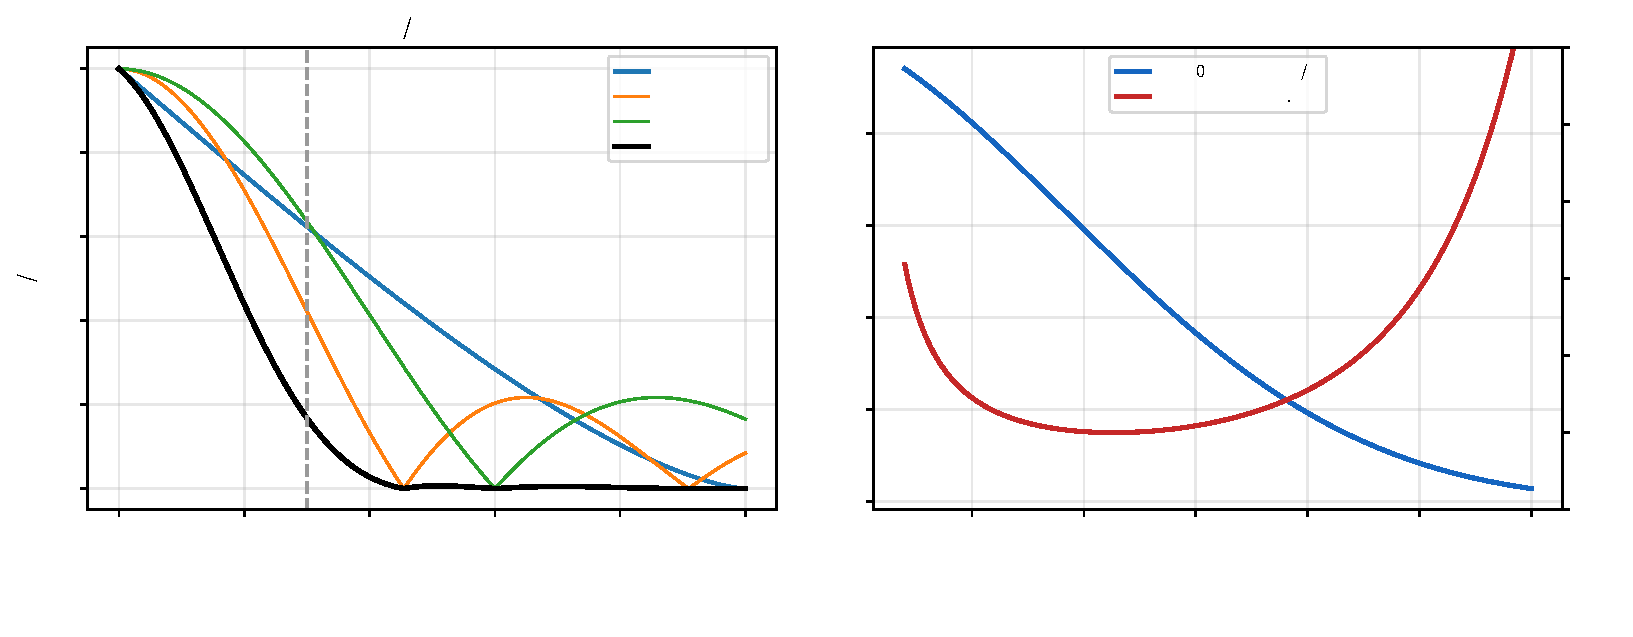
\includegraphics[width=0.98\textwidth]{fig-mtf-curve.pdf}
  \caption{左：衍射、离焦与像元 MTF 级联；右：链路 MTF 与相对深度噪声随条纹频率变化，存在最优区间（概念草图，非精确工程图）。}
  \label{fig:ch08-mtf}
\end{figure}

\subsection{链路 MTF、调制幅与相位噪声}

结构光中条纹经过两次成像：投影镜头把调制器上的图案成像到物面，相机镜头再把物面成像到传感器。物面的反射（含次表面散射）在中间又乘上一个「材料 $\MTF$」。设投影端条纹调制度为 $V_0$（第~\ref{ch:06}~章），相机所见调制度 $V=M/A$，平均灰度为 $A$，物面条纹频率为 $\xi$，则相机所见调制幅约为
\begin{equation}
  M(\xi)\approx A\,V_0\,\MTF_{\mathrm{proj}}(\xi)\,\MTF_{\mathrm{mat}}(\xi)\,\MTF_{\mathrm{cam}}(\xi).
  \label{eq:ch08-chain}
\end{equation}
代入第~\ref{ch:06}~章式~\eqref{eq:ch06-phase-noise}，$\sigma_\varphi\approx\sqrt{2/N}\,\sigma_I/M$。相位误差折算为物面横向位置误差为 $\delta x=\sigma_\varphi/(2\pi\xi)$，再经第~\ref{ch:07}~章的三角关系变成深度误差。于是
\begin{equation}
  \delta Z\ \propto\ \frac{1}{\xi\,\MTF_{\mathrm{link}}(\xi)}.
  \label{eq:ch08-tradeoff}
\end{equation}
提高条纹频率 $\xi$ 一方面使每弧度相位对应的位移更小（分母中的 $\xi$），另一方面使 $\MTF_{\mathrm{link}}$ 下降。二者乘积在某个中间频率处取最大，即深度噪声最小（图~\ref{fig:ch08-mtf} 右）。这给出选择条纹周期的光学依据，而不是「越密越好」。

\subsection{混合像素}

在深度不连续的边缘（牙齿轮廓、器械边缘），一个像元的 $\PSF$ 覆盖区域同时包含前景与背景。由于前后景的条纹相位不同，像元接收到的是两个复相量 $M_1e^{i\varphi_1}$ 与 $M_2e^{i\varphi_2}$ 按面积与亮度加权之和，求出的相位介于两者之间（甚至因相量抵消而 $M$ 很小），重建出漂浮在前后景之间的「飞点」。
高曲率表面虽然连续，但 $\PSF$ 覆盖区域内相位非线性变化，同样产生偏置，表现为尖锐边缘被「磨圆」、窄槽被「填浅」。$\PSF$ 越宽（离焦、低 $\MTF$），受影响的带宽越大。诊断特征：调制幅 $M$ 在边缘处骤降；相位梯度异常大。

\subsection{例：离焦怎样一步步吃掉调制度}

把模糊换算成调制度损失，就能直接接到第~\ref{ch:06}~章的相位噪声上。几何光学下，离焦 $\Delta z$ 在物方形成直径约
\[
  b\approx2\,\mathrm{NA}_o\,|\Delta z|
\]
的均匀圆斑（$\mathrm{NA}_o$ 为物方数值孔径；适用于离焦斑远大于衍射斑时）。均匀圆斑的 $\MTF$ 为
\[
  \MTF_{\mathrm{def}}(\xi)=\left|\frac{2J_1(\pi b\xi)}{\pi b\xi}\right|,
\]
小自变量时 $\approx1-(\pi b\xi)^2/8$。级联到式~\eqref{eq:ch08-cascade} 中，相机所见调制度 $V\approx V_0\cdot\MTF_{\mathrm{tot}}(\xi)$，相位噪声随 $1/V$ 增长。

\textbf{数量级示意。} 物方 $\mathrm{NA}_o=0.03$，条纹物方周期 $0.2\,\mathrm{mm}$（$\xi=5$ 周/mm）：
\begin{center}
\small
\begin{tabular}{cccc}
  \hline
  $|\Delta z|$ & $b$ & $\MTF_{\mathrm{def}}$ & $\sigma_\varphi$ 相对焦面\\
  \hline
  $0.5\,\mathrm{mm}$ & $30\,\mu\mathrm{m}$ & $0.97$ & $\times1.03$\\
  $1\,\mathrm{mm}$ & $60\,\mu\mathrm{m}$ & $0.89$ & $\times1.1$\\
  $2\,\mathrm{mm}$ & $120\,\mu\mathrm{m}$ & $0.62$ & $\times1.6$\\
  $3\,\mathrm{mm}$ & $180\,\mu\mathrm{m}$ & $0.28$ & $\times3.5$\\
  \hline
\end{tabular}
\end{center}
（$\pi b\xi=3.83$ 即 $b=244\,\mu\mathrm{m}$ 时 $\MTF$ 第一次降到零，条纹完全消失，之后出现反相的伪调制。）这里只算了相机侧离焦；投影侧同样离焦，两者相乘，实际下降更快。表中 $\Delta z=2\,\mathrm{mm}$ 一行与第~\ref{ch:01}~章算出的景深量级相当：景深边缘不是「清晰与模糊」的分界，而是相位噪声开始成倍增长的位置。

\subsection{例：混合像素的相量算一遍}

边缘像素中，前景面积占比 $\alpha$，前景与背景调制幅 $M_1$、$M_2$，相位差 $\Delta\varphi$。像素所得相量
\[
  \tilde M e^{i\tilde\varphi}=\alpha M_1e^{i\varphi_1}+(1-\alpha)M_2e^{i\varphi_2}.
\]
取 $\varphi_1=0$、$\alpha=0.5$、$M_1=3M_2$、$\Delta\varphi=1\,\mathrm{rad}$：
\[
  \tilde\varphi=\operatorname{atan2}\bigl(\sin1,\ 3+\cos1\bigr)=\operatorname{atan2}(0.841,\,3.540)\approx0.233\,\mathrm{rad}.
\]
面积各占一半，相位却只偏向背景 $0.233$ 而不是 $0.5\,\mathrm{rad}$：亮的一方「拉」住了相位。合成幅值 $\tilde M=0.5\times3.638M_2\approx1.82M_2$，比两者平均 $2M_2$ 低约 $9\%$，变化不大，因而单靠 $M$ 门限难以发现这种像素。若 $M_1=M_2$、$\Delta\varphi=\pi$，相量完全抵消，$\tilde M\to0$，此时 $M$ 门限能剔除它。所以混合像素有两种：抵消型（$M$ 骤降，易剔除）与偏置型（$M$ 基本正常，相位偏到一侧，需要用深度不连续检测或相位梯度判据）。

\subsection{去卷积能救回多少}

既然模糊是卷积（式~\eqref{eq:ch08-conv}），能否除以光学传递函数 复原？对结构光，关心的只是条纹基频 $\xi_0$ 处的幅度：除以 $\MTF(\xi_0)$ 能把 $M$ 恢复，但噪声同样被放大 $1/\MTF(\xi_0)$ 倍，$\SNR$ 不变，相位噪声也就不变。去卷积无法凭空恢复信噪比，它只在两种情况下有用：(i) 模糊在空间上变化（例如混合像素附近），复原能改善几何偏置；(ii) 需要的是图像外观而不是相位。对相位而言，真正的出口是让 $\MTF(\xi_0)$ 本身变大：选更长的条纹周期、更大的景深或对焦更准。

\section{限度}
\label{sec:ch08-limits}

\begin{itemize}
  \item 空间不变假设：真实镜头的 $\PSF$ 随视场与深度变化，$\MTF$ 应在多个视场点、多个深度分别给出；本章的单一曲线只是代表。
  \item 非相干成像假设：激光照明下系统对复振幅线性，传递函数是相干传递函数（截止频率为非相干的一半），且出现散斑。
  \item 级联相乘只对相互独立、线性的模糊环节成立；传感器饱和、伽马、二值化之后不再适用。
  \item 几何离焦 $\MTF$ 在弥散圆接近衍射斑时失效，需用波像差计算。
  \item 「材料 $\MTF$」是对次表面散射的粗略等效，忽略了它带来的相位偏移（第~\ref{ch:06}~章）。
\end{itemize}

\section{对象}
\label{sec:ch08-object}

\textbf{选条纹周期。} 设口内设备（数量级示意）：相机像元 $3\,\mu\mathrm{m}$、放大率 $0.3$，则物面像元约 $10\,\mu\mathrm{m}$；工作 F 数 $8$、蓝光。物面上条纹周期 $P_{\mathrm{obj}}$ 若取 $0.1\,\mathrm{mm}$（$10\,$周期/毫米），相当于每周期约 $10$ 个物面像元，像元 $\MTF$ 接近 $1$，衍射 $\MTF$ 仍高；但景深边缘弥散圆若达 $60\,\mu\mathrm{m}$（物面），离焦 $\MTF=2J_1(x)/x$ 在 $x=\pi c\xi\approx1.9$ 处约为 $0.6$，投影与相机两侧同时离焦则约 $0.36$，再叠加牙体散射，$M$ 可能只剩焦面处的三分之一左右。于是常见做法是：以\emph{景深边缘}而非焦面处的链路 $\MTF$ 来选周期，让边缘处 $M$ 仍高于展开可靠所需的阈值。

\textbf{模糊预算表。} 把每个环节在选定频率处的 $\MTF$ 列出（焦面 / 景深边缘两列）：投影衍射、投影离焦、材料、相机衍射、相机离焦、像元、运动。乘积给出 $M$ 的预期范围，再用式~\eqref{eq:ch06-phase-noise} 得到 $\sigma_\varphi$，用第~\ref{ch:07}~章的式~\eqref{eq:ch07-error} 得到 $\delta Z$。若结果超标，可从表中直接看出最差的一环：是离焦（需要更大景深或更小孔径）、是运动（需要更短曝光）、还是材料（需要更短波长或更低频率）。

\textbf{色差的实际影响。} 白光相机配蓝光投影：标定若用白光棋盘格，焦距与畸变系数会与蓝光工作状态略有差别，平面重建出现轻微碗形或尺度偏差。对策是用工作波长的照明进行标定，或在镜头设计中对工作波段做色差校正。

\section*{本章收束}
色散让焦距与畸变随波长变化，单色或窄带光源是结构光的常见选择。$\MTF$ 把模糊量化为「每个空间频率剩下多少调制度」，各环节级联相乘。调制幅 $M$ 是链路 $\MTF$ 的直接结果，因此条纹周期存在由光学决定的最优区间。边缘与高曲率处的混合像素来自 $\PSF$ 的有限宽度，是不可平均的系统误差。

\section{习题}
\label{sec:ch08-exercises}

\begin{enumerate}
  \item \textbf{（计算）} $\lambda=450\,\mathrm{nm}$、$N_F=5.6$ 与 $N_F=11$ 时衍射截止频率各为多少？对 $2.4\,\mu\mathrm{m}$ 像元，哪种情况下衍射成为奈奎斯特频率处的主导限制？
  \item \textbf{（计算）} 某频率处投影 $\MTF=0.7$、材料 $0.6$、相机 $0.8$、像元 $0.9$，投影端调制度 $V_0=0.9$，平均灰度 $A=120$。估算调制幅 $M$；若 $\sigma_I=2$、四步相移，求 $\sigma_\varphi$。
  \item \textbf{（重建场景）} 同一台设备在焦面处精度很好，在景深边缘噪声增加三倍以上，且条纹越密越明显。用 $\MTF$ 级联解释。
  \item \textbf{（重建场景）} 牙齿轮廓边缘一圈出现漂浮点，位于牙面与背景之间。原因是什么？给出基于 $M$ 和相位梯度的剔除规则。
  \item \textbf{（重建场景）} 换用另一颜色的投影光源后，未重新标定，平面重建出现轻微碗形。解释并给出对策。
  \item \textbf{（设计）} 由式~\eqref{eq:ch08-tradeoff}，若 $\MTF_{\mathrm{link}}(\xi)\approx1-\xi/\xi_0$（线性近似），求使 $\delta Z$ 最小的 $\xi$。
  \item \textbf{（诊断）} 相位误差图在某些区域条纹相位整体反转了约 $\pi$，而调制幅很低。可能是离焦 $\MTF$ 的什么现象？
  \item \textbf{（推导）} 由均匀圆斑的 $\MTF$ 小自变量展开，求 $\MTF_{\mathrm{def}}$ 降到 $0.9$ 时 $b\xi$ 的值，并给出对应的离焦量公式。
  \item \textbf{（计算）} 正文表中若条纹周期加长到 $0.4\,\mathrm{mm}$，$\Delta z=2\,\mathrm{mm}$ 时 $\MTF_{\mathrm{def}}$ 约为多少？代价是什么（结合第~\ref{ch:06}~章 $\delta d=P\sigma_\varphi/2\pi$）？
  \item \textbf{（口扫场景）} 牙齿邻接面边缘，前景牙面 $M_1=M_2$，$\alpha=0.3$，$\Delta\varphi=2\,\mathrm{rad}$。求合成相位与幅值；按 $P=16$ 像素换算为多少像素的投影坐标偏差？
  \item \textbf{（医学重建）} 内镜结构光中组织表面有一层液膜，使边缘出现强镜面高光（$M_1=10M_2$）。在 $\alpha$ 只有 $0.1$ 时，相位偏向高光一侧多少（$\Delta\varphi=1\,\mathrm{rad}$）？说明这对边缘几何的影响。
  \item \textbf{（C++/CUDA 实践）} 设计一个检测偏置型混合像素的 GPU 后处理：给出所用判据（相位梯度、深度跳变、$M$ 局部比值），以及邻域访问如何用共享内存实现。
\end{enumerate}

\section{习题讲解}
\label{sec:ch08-solutions}

\begin{enumerate}
  \item $\xi_c=1/(\lambda N_F)$：$N_F=5.6$ 时约 $397$，$N_F=11$ 时约 $202\,$周期/毫米。$2.4\,\mu\mathrm{m}$ 像元奈奎斯特约 $208\,$周期/毫米。$N_F=11$ 时截止频率已低于奈奎斯特，衍射主导。
  \item 链路 $\MTF=0.7\times0.6\times0.8\times0.9\approx0.30$；$M\approx120\times0.9\times0.30\approx33$。$\sigma_\varphi\approx\sqrt{2/4}\times2/33\approx0.043\,\mathrm{rad}$。
  \item 景深边缘离焦 $\MTF$ 大幅下降，投影与相机两侧同时离焦，且乘积随频率下降更快；$M$ 下降导致 $\sigma_\varphi$ 上升。条纹越密，离焦 $\MTF$ 越低，效应越强。
  \item 混合像素：$\PSF$ 跨越深度不连续，前后景相量叠加，求出中间相位。规则：剔除 $M$ 低于阈值（如局部中值的一定比例）或相位梯度超过可能表面坡度上限的像素；或检查邻域深度跳变后剔除边缘带。
  \item 轴向与垂轴色差：焦距与畸变系数随波长变化，标定参数不再匹配，残余畸变表现为碗形。对策：以工作波长重新标定，或使用色差校正的镜头。
  \item $\xi\,\MTF=\xi-\xi^2/\xi_0$ 在 $\xi=\xi_0/2$ 时取最大，此时 $\delta Z$ 最小。
  \item 离焦 $\MTF$ 过零后的负值区：对比度反转，相位翻转 $\pi$，同时幅值小。说明该区域严重离焦，应降低条纹频率或剔除。
  \item $1-x^2/8=0.9$ 得 $x=\pi b\xi\approx0.894$，$b\xi\approx0.285$；由 $b=2\mathrm{NA}_o|\Delta z|$，$|\Delta z|\approx0.142/(\mathrm{NA}_o\xi)$。$\mathrm{NA}_o=0.03$、$\xi=5$ 时约 $0.95\,\mathrm{mm}$，与表中 $1\,\mathrm{mm}$ 一行一致。
  \item $\xi=2.5$，$\pi b\xi=0.942$，$\MTF\approx1-0.111=0.89$（准确值约 $0.89$）。代价：$P$ 加倍，同样 $\sigma_\varphi$ 下 $\delta d$ 加倍；景深边缘处相位噪声减为约 $0.62/0.89$，综合后约 $2\times0.70=1.4$ 倍，焦面处则直接是 $2$ 倍。周期选择是景深与焦面精度的权衡。
  \item 相量 $0.3+0.7e^{2i}=0.3+0.7(-0.416+0.909i)=0.009+0.636i$，$\tilde\varphi\approx1.56\,\mathrm{rad}$，$\tilde M\approx0.64M_1$。相对前景偏 $1.56\,\mathrm{rad}$，约 $16\times1.56/6.28\approx4$ 像素。面积只占七成的背景主导了相位。
  \item $0.1\times10+0.9e^{i}=1+0.486+0.757i$，$\tilde\varphi=\operatorname{atan2}(0.757,1.486)\approx0.47\,\mathrm{rad}$。背景相位为 $1\,\mathrm{rad}$，合成相位被拉向高光约 $0.53\,\mathrm{rad}$：只占一成面积的高光把相位拉过了一半。边缘轮廓会向高光一侧「外扩」，表现为组织边缘鼓起。
  \item 判据：$|\nabla\varphi|$ 超过正常条纹梯度的若干倍；相邻深度跳变大于预设阈值；像素 $M$ 与邻域中位数之比偏离（抵消型低于 $0.5$）。实现：每个线程块把 $(16+2)\times(16+2)$ 的相位与 $M$ 瓦片载入共享内存（含一像素边框），同步后每线程计算梯度与邻域统计，标记可疑像素；被标记像素可剔除或在深度跳变两侧按最近侧填补。
\end{enumerate}

\chapter{深度传感对照：共聚焦 / OCT / ToF}
\label{ch:09}

本章为选读。它不展开这些技术的全部细节，而是用前面各章的光学语言说明：它们各自靠什么获得深度，分辨率与量程由什么决定，以及与结构光、立体视觉的能力边界在哪里。

\section{效果}
\label{sec:ch09-effect}

读完本章，你应能：
\begin{enumerate}
  \item 说明共聚焦针孔如何实现光学层切，以及轴向分辨率与数值孔径的关系；
  \item 用第~\ref{ch:03}~章的相干长度解释 OCT 的轴向分辨率与量程；
  \item 区分脉冲 ToF 与相位（调幅连续波）ToF，写出相位 ToF 的距离公式与无模糊量程；
  \item 用一张对照表比较五类深度传感的分辨率、量程、对材料的敏感性与系统代价；
  \item 理解口内扫描常见选型背后的取舍。
\end{enumerate}

\section{原理}
\label{sec:ch09-principle}

\subsection{共聚焦：用针孔挑出焦面}

共聚焦系统把点光源聚焦到样品，再把返回光聚焦到与光源共轭的针孔上。焦面上的点回到针孔中心，全部通过；焦面外的点在针孔处是一个弥散斑，只有少部分通过。沿光轴扫描焦面（或扫描物体），记录每个横向位置的信号最大值所在深度，即得表面高度 \citep{WilsonSheppard1984}。

轴向响应宽度（层切厚度）近似
\begin{equation}
  \Delta z_{\mathrm{conf}}\sim\frac{\lambda}{\mathrm{NA}^2}
  \label{eq:ch09-conf}
\end{equation}
（常数因子依赖针孔大小与定义，量级为 $0.5$--$1.5$）。与第~\ref{ch:01}~章的景深同源：$\NA$ 越大，焦面外越快模糊，层切越薄。

要点：
\begin{itemize}
  \item 深度来自\emph{焦点位置}，不需要三角基线，因此可以在很窄的探头里工作，遮挡少（照明与观测同轴）。
  \item 量程由焦面扫描行程决定；精度由轴向响应宽度与 $\SNR$ 决定，峰值插值可达响应宽度的一小部分。
  \item 并行化：用针孔阵列或光栅图案配合深度扫描，可一次获得一片区域，代价是串扰与扫描时间。
  \item 半透明材料内部的散射光被针孔大量拒绝，这是共聚焦对次表面散射天然较鲁棒的原因。
\end{itemize}

\subsection{OCT：低相干干涉}

光学相干层析（OCT）把样品臂与参考臂的反射光在探测器上干涉 \citep{Huang1991OCT}。光源是宽带低相干光（第~\ref{ch:03}~章）：只有两臂光程差小于相干长度 $l_c$ 时才出现干涉条纹。因此干涉信号的包络定位了「样品中哪一深度的反射与参考臂等光程」。

对高斯谱、中心波长 $\lambda_0$、半高宽 $\Delta\lambda$ 的光源，轴向分辨率（空气中）为
\begin{equation}
  \Delta z_{\mathrm{OCT}}=\frac{2\ln2}{\pi}\,\frac{\lambda_0^{2}}{\Delta\lambda}.
  \label{eq:ch09-oct}
\end{equation}
例：$\lambda_0=840\,\mathrm{nm}$、$\Delta\lambda=50\,\mathrm{nm}$，$\Delta z\approx6.2\,\mu\mathrm{m}$；在折射率 $n$ 的介质中再除以 $n$。注意它与\emph{横向}分辨率解耦：横向由聚焦 $\NA$ 决定，轴向由光谱宽度决定。

\begin{itemize}
  \item \textbf{时域 OCT}：机械扫描参考臂长度。
  \item \textbf{频域 OCT}：参考臂固定，用光谱仪或扫频光源记录干涉光谱，傅里叶变换得到整条深度剖面。量程由光谱采样间隔决定，$z_{\max}\approx\lambda_0^2/(4\,\delta\lambda)$（$\delta\lambda$ 为每个光谱采样的宽度）。
\end{itemize}
OCT 的独特能力是\emph{看进去}：给出组织内部多层界面的反射，而不仅是表面。代价是量程浅（毫米级）、需要逐点或逐线扫描、系统复杂。

\subsection{ToF：飞行时间}

\textbf{脉冲 ToF}：发出短脉冲，测量往返时间 $\Delta t$，$Z=c\Delta t/2$。$1\,\mathrm{mm}$ 深度对应约 $6.7\,\mathrm{ps}$ 往返时间，可见毫米级精度需要皮秒级时间分辨。

\textbf{相位 ToF（调幅连续波）}：光源强度按调制频率 $F_m$（角频率 $\omega_m=2\pi F_m$；注意：$F_m$ 是强度包络的调制频率，通常为数十兆赫兹，远低于光频 $\nu$）正弦调制。返回光相对发射光有相位延迟 $\phi_m$，则
\begin{equation}
  Z=\frac{c}{4\pi F_m}\,\phi_m,\qquad Z_{\mathrm{amb}}=\frac{c}{2F_m}.
  \label{eq:ch09-tof}
\end{equation}
$Z_{\mathrm{amb}}$ 为无模糊量程：$F_m=20\,\mathrm{MHz}$ 时约 $7.5\,\mathrm{m}$。相位通常由每像素四个相位采样求得，形式与第~\ref{ch:06}~章的四步相移完全相同 \citep{LangeSeitz2001ToF}，于是深度噪声
\[
  \sigma_Z\approx\frac{c}{4\pi F_m}\,\sigma_{\phi_m},
\]
$\sigma_{\phi_m}$ 同样反比于调制幅与 $\SNR$。这里的「条纹」不在空间而在时间上：$c/(2F_m)$ 扮演条纹周期的角色。即便 $F_m=100\,\mathrm{MHz}$，周期也有 $1.5\,\mathrm{m}$，$0.01\,\mathrm{rad}$ 相位噪声对应约 $2.4\,\mathrm{mm}$。这解释了 ToF 在近距离精细测量上的根本劣势。多频 ToF 展开相位的思路与第~\ref{ch:06}~章多频外差相同。

ToF 的典型误差：多径干扰（墙角、凹面中光经过多次反射，等价于结构光的互反射）、次表面散射造成的延迟、混合像素（边缘飞点），以及温度引起的相位漂移。

\subsection{能力边界对照}

\begin{table}[htbp]
  \centering
  \small
  \begin{tabular}{@{}p{0.10\textwidth}p{0.12\textwidth}p{0.19\textwidth}p{0.19\textwidth}p{0.22\textwidth}@{}}
    \toprule
    方式 & 深度来源 & 轴向分辨率（量级） & 量程（量级） & 主要限制 \\
    \midrule
    共聚焦 & 焦点位置 & $1$--$20\,\mu\mathrm{m}$ & $0.1$--$20\,\mathrm{mm}$ & 扫描时间、$\NA$ 与视场 \\
    OCT & 相干门 & $2$--$10\,\mu\mathrm{m}$ & $0.5$--$5\,\mathrm{mm}$ & 量程浅、逐点扫描 \\
    结构光 & 三角+相位 & $3$--$50\,\mu\mathrm{m}$ & $1$--$500\,\mathrm{mm}$ & $\MTF$、散射、遮挡 \\
    立体 & 三角+匹配 & $10\,\mu\mathrm{m}$--$1\,\mathrm{mm}$ & $1\,\mathrm{mm}$--$20\,\mathrm{m}$ & 纹理、基线 \\
    ToF & 往返时间 & $1$--$30\,\mathrm{mm}$ & $0.1$--$20\,\mathrm{m}$ & 多径、时间分辨 \\
    \bottomrule
  \end{tabular}
  \caption{深度传感方式能力边界（数量级示意，非具体产品指标）。}
  \label{tab:ch09-compare}
\end{table}

图~\ref{fig:ch09-compare} 把同样的信息画在分辨率–量程平面上。可以看到一条大致规律：\emph{深度分辨率与量程之比}大体被各自的「编码尺度」锁定——共聚焦是焦深，OCT 是相干长度，结构光是条纹周期与基线，ToF 是调制周期。

\begin{figure}[htbp]
  \centering
  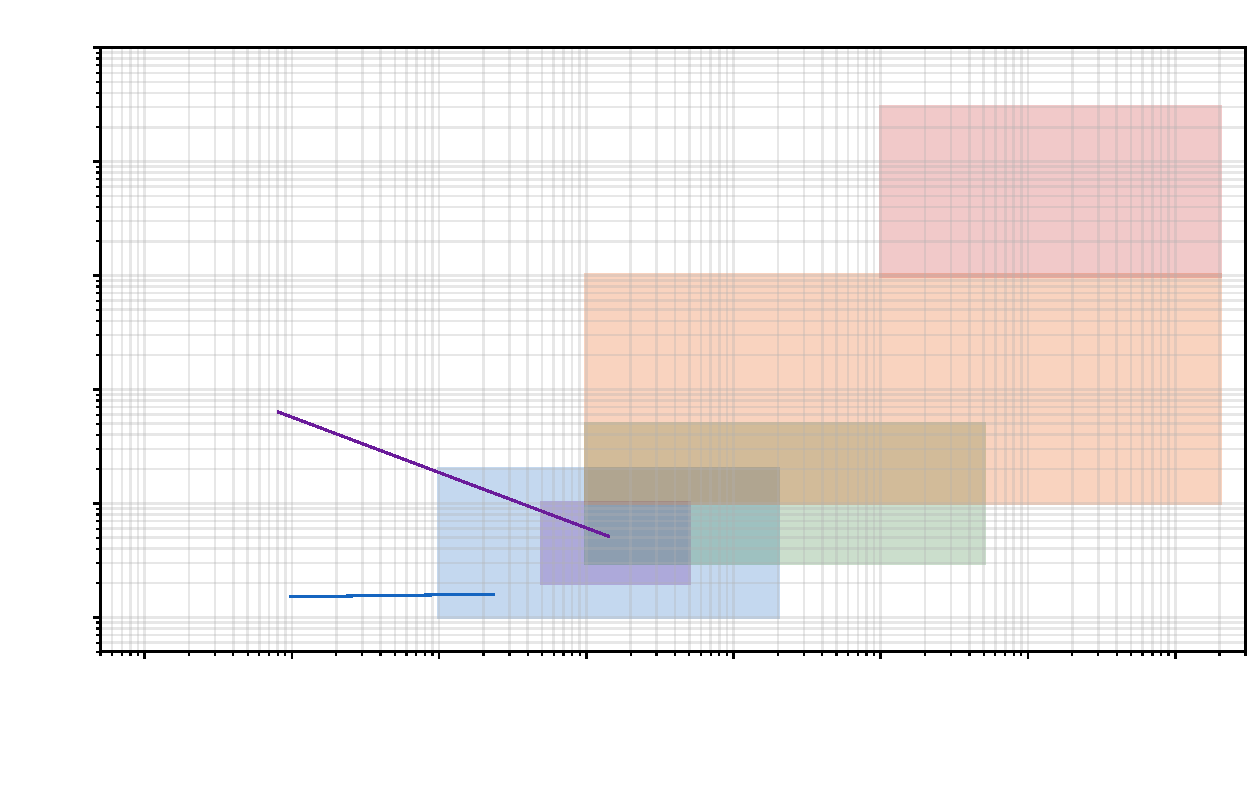
\includegraphics[width=0.85\textwidth]{fig-sensor-compare.pdf}
  \caption{各深度传感方式在分辨率–量程平面上的大致位置（概念草图，数量级示意）。}
  \label{fig:ch09-compare}
\end{figure}

\section{限度}
\label{sec:ch09-limits}

\begin{itemize}
  \item 式~\eqref{eq:ch09-conf}、\eqref{eq:ch09-oct} 的常数因子依赖定义（半高宽、针孔尺寸、谱形），只能做量级比较。
  \item 对照表忽略了速度、成本、体积与安全（激光功率）等维度，它们往往决定实际选型。
  \item 介质折射率改变光程：OCT 与 ToF 测得的是光程而非几何距离；半透明材料中共聚焦与结构光也会受到影响。
  \item 本章不涉及光度立体、焦点堆栈（depth from focus）等其他方法，它们与共聚焦或立体的原理相近。
\end{itemize}

\section{对象}
\label{sec:ch09-object}

\textbf{口内扫描常见选型（数量级示意）。} 口内场景的约束是：工作距十余毫米、深度范围数毫米到十余毫米、探头狭小、手持移动、表面湿润且半透明、精度目标数十微米。
\begin{itemize}
  \item \textbf{结构光}（相机+投影或多相机+条纹）：帧率高，单帧覆盖面积大，便于拼接；短板是散射与高反（第~\ref{ch:06}~章），以及基线受探头尺寸限制（第~\ref{ch:07}~章）。
  \item \textbf{并行共聚焦}：同轴、无遮挡、对散射较鲁棒，适合深窄的龈沟与邻面；但需要焦面扫描，单帧时间较长，对运动敏感，探头光学更复杂。
  \item \textbf{OCT}：能看到釉质下的结构（龋损、修复体界面），研究价值大；作为全牙弓表面扫描，量程与速度不足。
  \item \textbf{ToF}：精度远不够口内要求，主要见于房间尺度或人体尺度的测量。
\end{itemize}
不同产品的取舍差异主要在：用多少帧换精度、用什么方式对付散射与高反、探头允许的基线与景深。

\section*{本章收束}
共聚焦用焦点，OCT 用相干门，ToF 用往返时间，结构光与立体用三角。每种方法都有一个「编码尺度」，分辨率是这个尺度的一小部分，量程是它的若干倍。相位 ToF 与相移结构光在数学上同构，只是一个在时间上、一个在空间上编码。口内扫描以结构光与并行共聚焦为主，取舍落在速度、散射鲁棒性与探头尺寸上。

\section{习题}
\label{sec:ch09-exercises}

\begin{enumerate}
  \item \textbf{（计算）} 共聚焦物镜 $\NA=0.3$、$\lambda=488\,\mathrm{nm}$，估算层切厚度量级。若改为 $\NA=0.1$ 呢？对口内全牙扫描意味着什么？
  \item \textbf{（计算）} OCT 光源 $\lambda_0=1300\,\mathrm{nm}$、$\Delta\lambda=100\,\mathrm{nm}$，求空气中与牙釉质（$n\approx1.6$）中的轴向分辨率。
  \item \textbf{（计算）} 相位 ToF $F_m=60\,\mathrm{MHz}$，求无模糊量程；若相位噪声 $0.005\,\mathrm{rad}$，深度噪声多少？与口内精度目标对比。
  \item \textbf{（重建场景）} 在深而窄的龈沟中，结构光扫描缺失严重而共聚焦扫描较完整。从光路几何解释。
  \item \textbf{（重建场景）} ToF 相机拍摄墙角时，角落深度系统性偏大且角落被「磨圆」。原因是什么？它与结构光中的哪种误差同源？
  \item \textbf{（设计）} 若要检测修复体边缘下方的微小间隙（数十微米、位于表面下方），应考虑哪种方法？说明理由与代价。
\end{enumerate}

\section{习题讲解}
\label{sec:ch09-solutions}

\begin{enumerate}
  \item $\lambda/\NA^2\approx0.488/0.09\approx5.4\,\mu\mathrm{m}$；$\NA=0.1$ 时约 $49\,\mu\mathrm{m}$。$\NA$ 大层切薄、精度高，但视场与景深小，需要更长的扫描行程与时间；口内常取中等 $\NA$ 折中。
  \item $\Delta z=0.44\times1300^2/100\,\mathrm{nm}\approx7.5\,\mu\mathrm{m}$（空气），釉质中约 $4.7\,\mu\mathrm{m}$。
  \item $Z_{\mathrm{amb}}=c/(2F_m)=2.5\,\mathrm{m}$；$\sigma_Z=c\sigma_{\phi_m}/(4\pi F_m)\approx3\times10^8\times0.005/(4\pi\times6\times10^7)\approx2\,\mathrm{mm}$，比口内目标大约两个数量级。
  \item 结构光需要投影与相机两个方向都能看到沟底，基线带来阴影与遮挡；共聚焦照明与观测同轴，只要一个方向能看到即可。
  \item 多径干扰：光在两面墙之间多次反射后返回，路径更长，相位延迟偏大。与结构光中的互反射同源，都违反「每像素只接收一次直接反射」的假设。
  \item OCT：能分辨表面以下的界面，轴向分辨率数微米。代价：量程浅、扫描慢、系统复杂，需与表面扫描配合使用。
\end{enumerate}

\chapter{深度传感对照：共聚焦 / OCT / ToF}
\label{ch:10}

本章为选读。它不展开这些技术的全部细节，而是用前面各章的光学语言说明：它们各自靠什么获得深度，分辨率与量程由什么决定，以及与结构光、立体视觉的能力边界在哪里。

\section{效果}
\label{sec:ch09-effect}

读完本章，你应能：
\begin{enumerate}
  \item 说明共聚焦针孔如何实现光学层切，以及轴向分辨率与数值孔径的关系；
  \item 用第~\ref{ch:04}~章的相干长度解释 OCT 的轴向分辨率与量程；
  \item 区分脉冲 ToF 与相位（调幅连续波）ToF，写出相位 ToF 的距离公式与无模糊量程；
  \item 用一张对照表比较五类深度传感的分辨率、量程、对材料的敏感性与系统代价；
  \item 理解口内扫描常见选型背后的取舍。
\end{enumerate}

\section{原理}
\label{sec:ch09-principle}

\subsection{共聚焦：用针孔挑出焦面}

共聚焦系统把点光源聚焦到样品，再把返回光聚焦到与光源共轭的针孔上。焦面上的点回到针孔中心，全部通过；焦面外的点在针孔处是一个弥散斑，只有少部分通过。沿光轴扫描焦面（或扫描物体），记录每个横向位置的信号最大值所在深度，即得表面高度 \citep{WilsonSheppard1984}。

轴向响应宽度（层切厚度）近似
\begin{equation}
  \Delta z_{\mathrm{conf}}\sim\frac{\lambda}{\mathrm{NA}^2}
  \label{eq:ch10-conf}
\end{equation}
（常数因子依赖针孔大小、折射率与定义：理想小针孔、小 $\NA$ 时轴向响应半高宽约 $1.3\,n\lambda/\NA^2$，针孔变大则变宽；此处只作量级比较）。与第~\ref{ch:01}~章的景深同源：$\NA$ 越大，焦面外越快模糊，层切越薄。

要点：
\begin{itemize}
  \item 深度来自\emph{焦点位置}，不需要三角基线，因此可以在很窄的探头里工作，遮挡少（照明与观测同轴）。
  \item 量程由焦面扫描行程决定；精度由轴向响应宽度与 $\SNR$ 决定，峰值插值可达响应宽度的一小部分。
  \item 并行化：用针孔阵列或光栅图案配合深度扫描，可一次获得一片区域，代价是串扰与扫描时间。
  \item 半透明材料内部的散射光被针孔大量拒绝，这是共聚焦对次表面散射天然较鲁棒的原因。
\end{itemize}

\subsection{OCT：低相干干涉}

光学相干层析（OCT）把样品臂与参考臂的反射光在探测器上干涉 \citep{Huang1991OCT}。光源是宽带低相干光（第~\ref{ch:04}~章）：只有两臂光程差小于相干长度 $l_c$ 时才出现干涉条纹。因此干涉信号的包络定位了「样品中哪一深度的反射与参考臂等光程」。

对高斯谱、中心波长 $\lambda_0$、半高宽 $\Delta\lambda$ 的光源，轴向分辨率（空气中）为
\begin{equation}
  \Delta z_{\mathrm{OCT}}=\frac{2\ln2}{\pi}\,\frac{\lambda_0^{2}}{\Delta\lambda}.
  \label{eq:ch10-oct}
\end{equation}
例：$\lambda_0=840\,\mathrm{nm}$、$\Delta\lambda=50\,\mathrm{nm}$，$\Delta z\approx6.2\,\mu\mathrm{m}$；在折射率 $n$ 的介质中再除以 $n$。注意它与\emph{横向}分辨率解耦：横向由聚焦 $\NA$ 决定，轴向由光谱宽度决定。

\begin{itemize}
  \item \textbf{时域 OCT}：机械扫描参考臂长度。
  \item \textbf{频域 OCT}：参考臂固定，用光谱仪或扫频光源记录干涉光谱，傅里叶变换得到整条深度剖面。量程由光谱采样间隔决定，$z_{\max}\approx\lambda_0^2/(4\,\delta\lambda)$（$\delta\lambda$ 为每个光谱采样的宽度）。
\end{itemize}
OCT 的独特能力是\emph{看进去}：给出组织内部多层界面的反射，而不仅是表面。代价是量程浅（毫米级）、需要逐点或逐线扫描、系统复杂。

\subsection{ToF：飞行时间}

\textbf{脉冲 ToF}：发出短脉冲，测量往返时间 $\Delta t$，$Z=c\Delta t/2$（本章 $c$ 为光速，不同于第~\ref{ch:01}~章的弥散圆直径）。$1\,\mathrm{mm}$ 深度对应约 $6.7\,\mathrm{ps}$ 往返时间，可见毫米级精度需要皮秒级时间分辨。

\textbf{相位 ToF（调幅连续波）}：光源强度按调制频率 $F_m$（角频率 $\omega_m=2\pi F_m$；注意：$F_m$ 是强度包络的调制频率，通常为数十兆赫兹，远低于光频 $\nu$）正弦调制。返回光相对发射光有相位延迟 $\phi_m$，则
\begin{equation}
  Z=\frac{c}{4\pi F_m}\,\phi_m,\qquad Z_{\mathrm{amb}}=\frac{c}{2F_m}.
  \label{eq:ch10-tof}
\end{equation}
$Z_{\mathrm{amb}}$ 为无模糊量程：$F_m=20\,\mathrm{MHz}$ 时约 $7.5\,\mathrm{m}$。相位通常由每像素四个相位采样求得，形式与第~\ref{ch:07}~章的四步相移完全相同 \citep{LangeSeitz2001ToF}，于是深度噪声
\[
  \sigma_Z\approx\frac{c}{4\pi F_m}\,\sigma_{\phi_m},
\]
$\sigma_{\phi_m}$ 同样反比于调制幅与 $\SNR$。这里的「条纹」不在空间而在时间上：$c/(2F_m)$ 扮演条纹周期的角色。即便 $F_m=100\,\mathrm{MHz}$，周期也有 $1.5\,\mathrm{m}$，$0.01\,\mathrm{rad}$ 相位噪声对应约 $2.4\,\mathrm{mm}$。这解释了 ToF 在近距离精细测量上的根本劣势。多频 ToF 展开相位的思路与第~\ref{ch:07}~章多频外差相同。

ToF 的典型误差：多径干扰（墙角、凹面中光经过多次反射，等价于结构光的互反射）、次表面散射造成的延迟、混合像素（边缘飞点），以及温度引起的相位漂移。

\subsection{能力边界对照}

\begin{table}[htbp]
  \centering
  \small
  \begin{tabular}{@{}p{0.10\textwidth}p{0.12\textwidth}p{0.19\textwidth}p{0.19\textwidth}p{0.22\textwidth}@{}}
    \toprule
    方式 & 深度来源 & 轴向分辨率（量级） & 量程（量级） & 主要限制 \\
    \midrule
    共聚焦 & 焦点位置 & $1$--$20\,\mu\mathrm{m}$ & $0.1$--$20\,\mathrm{mm}$ & 扫描时间、$\NA$ 与视场 \\
    OCT & 相干门 & $2$--$10\,\mu\mathrm{m}$ & $0.5$--$5\,\mathrm{mm}$ & 量程浅、逐点扫描 \\
    结构光 & 三角+相位 & $3$--$50\,\mu\mathrm{m}$ & $1$--$500\,\mathrm{mm}$ & $\MTF$、散射、遮挡 \\
    立体 & 三角+匹配 & $10\,\mu\mathrm{m}$--$1\,\mathrm{mm}$ & $1\,\mathrm{mm}$--$20\,\mathrm{m}$ & 纹理、基线 \\
    ToF & 往返时间 & $1$--$30\,\mathrm{mm}$ & $0.1$--$20\,\mathrm{m}$ & 多径、时间分辨 \\
    \bottomrule
  \end{tabular}
  \caption{深度传感方式能力边界（数量级示意，非具体产品指标）。}
  \label{tab:ch09-compare}
\end{table}

图~\ref{fig:ch10-compare} 把同样的信息画在分辨率–量程平面上。可以看到一条大致规律：\emph{深度分辨率与量程之比}大体被各自的「编码尺度」锁定——共聚焦是焦深，OCT 是相干长度，结构光是条纹周期与基线，ToF 是调制周期。

\begin{figure}[htbp]
  \centering
  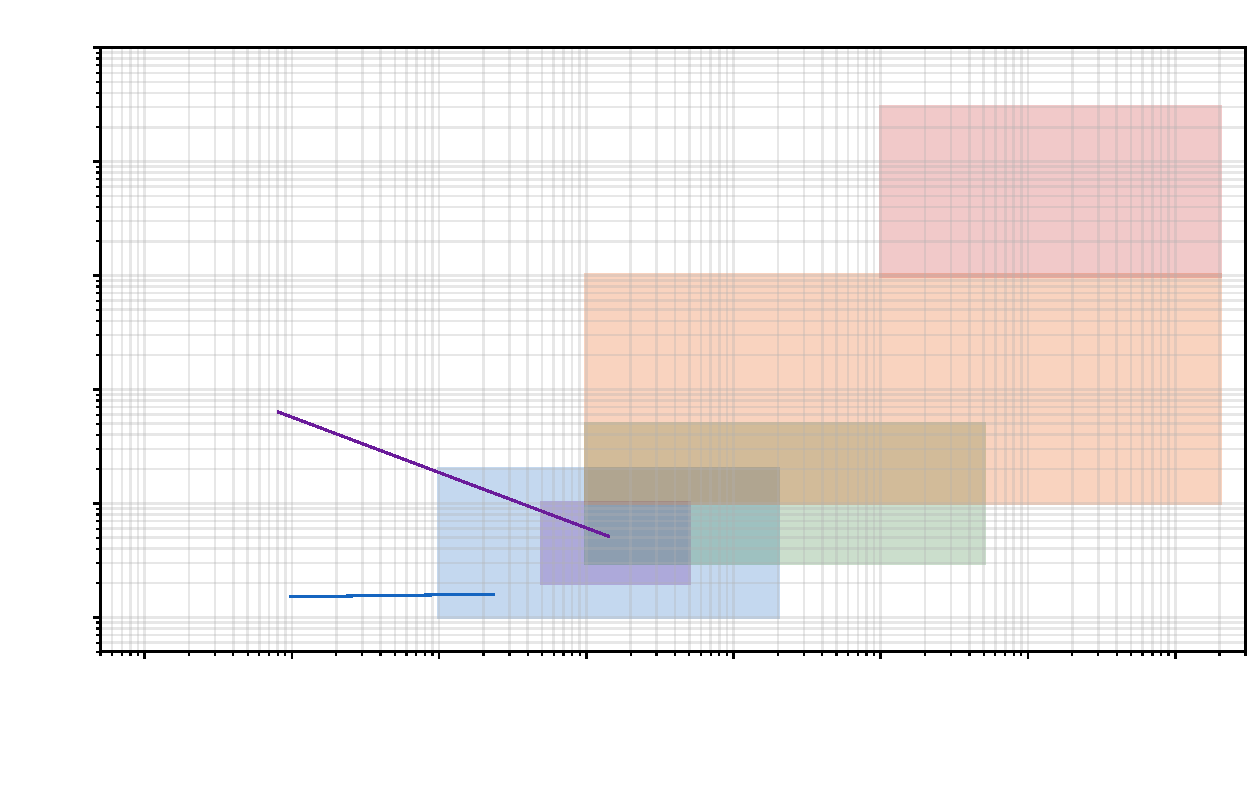
\includegraphics[width=0.85\textwidth]{fig-sensor-compare.pdf}
  \caption{各深度传感方式在分辨率–量程平面上的大致位置（概念草图，数量级示意）。}
  \label{fig:ch10-compare}
\end{figure}

\subsection{例：OCT 轴向分辨率与深度范围}

式~\eqref{eq:ch10-oct} 的轴向分辨率（高斯谱、半高全宽定义）
\[
  \Delta z=\frac{2\ln2}{\pi}\,\frac{\lambda_0^2}{\Delta\lambda}.
\]
数量级示意：$\lambda_0=840\,\mathrm{nm}$、$\Delta\lambda=50\,\mathrm{nm}$，$\Delta z\approx0.441\times0.706/0.05\approx6.2\,\mu\mathrm{m}$（空气中）。组织中光程按折射率 $n\approx1.38$ 缩短，物理深度分辨率约 $6.2/1.38\approx4.5\,\mu\mathrm{m}$。注意它只取决于光谱宽度，与物镜 $\mathrm{NA}$ 无关；横向分辨率才由 $\mathrm{NA}$ 决定。这是 OCT 能用低 $\mathrm{NA}$（大景深）同时得到微米级轴向分辨率的原因。

\textbf{频域 OCT 的深度范围。} 频域 OCT 用光谱仪记录干涉谱，深度剖面是谱的傅里叶变换。光谱仪每像素的波长间隔 $\delta\lambda_s$ 决定最大成像深度（单侧）
\[
  z_{\max}=\frac{\lambda_0^2}{4n\,\delta\lambda_s}.
\]
推导要点：干涉谱在波数 $k=2\pi/\lambda$ 上以 $\cos(2kz)$ 振荡，采样间隔 $\delta k=2\pi\delta\lambda_s/\lambda_0^2$，奈奎斯特条件 $2z\,\delta k\le\pi$。例：$2048$ 像素覆盖 $100\,\mathrm{nm}$，$\delta\lambda_s\approx0.049\,\mathrm{nm}$，空气中 $z_{\max}\approx0.706/(4\times4.9\times10^{-5})\,\mu\mathrm{m}\approx3.6\,\mathrm{mm}$。深度范围与分辨率共用同一组光谱像素：像素数固定时，覆盖更宽光谱（分辨率更好）就意味着 $\delta\lambda_s$ 更大、深度更浅。此外，光谱仪本身的有限分辨率使信号随深度衰减（称为滚降），实际可用深度短于 $z_{\max}$。

\subsection{例：共聚焦层析厚度}

按正文针孔足够小、$\mathrm{NA}$ 不大时的近似，轴向层析厚度约 $1.3\,n\lambda/\mathrm{NA}^2$。$\mathrm{NA}=0.3$、$\lambda=0.45\,\mu\mathrm{m}$、空气中：$1.3\times0.45/0.09\approx6.5\,\mu\mathrm{m}$。$\mathrm{NA}$ 减半到 $0.15$，层析厚度变为四倍约 $26\,\mu\mathrm{m}$。与 OCT 对比：共聚焦的轴向分辨率由 $\mathrm{NA}^2$ 决定，要微米级就要大 $\mathrm{NA}$，于是工作距离短、视场小、需要轴向扫描；口内共聚焦方案用平行多点阵列与轴向扫描换取视场，这是它与相移结构光在帧数与机械复杂度上的主要差别。

\subsection{例：ToF 的多径与多频}

本章已算过 $F_m=100\,\mathrm{MHz}$ 时无歧义距离 $1.5\,\mathrm{m}$ 与相位噪声对应的距离噪声。这里补两个系统项。

\textbf{多径。} 像素同时收到直接回波（幅值 $1$）与经墙角等二次反射的回波（幅值 $\beta$），后者往返总路程多出 $\Delta L$。连续波 ToF 的相位正比于往返路程，二者相位差 $\Delta\phi=2\pi F_m\Delta L/c$（此处 $c$ 为光速）。与混合像素同理，合成相位
\[
  \delta\phi=\operatorname{atan2}\bigl(\beta\sin\Delta\phi,\ 1+\beta\cos\Delta\phi\bigr).
\]
数量级示意：$\beta=0.2$、$\Delta L=0.3\,\mathrm{m}$，$\Delta\phi\approx0.63\,\mathrm{rad}$，$\delta\phi\approx0.10\,\mathrm{rad}$，换算距离 $c\,\delta\phi/(4\pi F_m)\approx2.4\,\mathrm{cm}$，比典型随机噪声大一个数量级，且总是使距离偏远。多径误差随 $F_m$ 变化（$\Delta\phi$ 正比于 $F_m$），这正是多频测量能识别多径的依据。

\textbf{多频去歧义。} 用 $80\,\mathrm{MHz}$ 与 $100\,\mathrm{MHz}$ 两个频率，二者公约数 $20\,\mathrm{MHz}$，组合后无歧义距离 $c/(2\times20\,\mathrm{MHz})=7.5\,\mathrm{m}$。逻辑与第~\ref{ch:07}~章外差完全相同，噪声放大与跳级风险也同理。

\section{限度}
\label{sec:ch09-limits}

\begin{itemize}
  \item 式~\eqref{eq:ch10-conf}、\eqref{eq:ch10-oct} 的常数因子依赖定义（半高宽、针孔尺寸、谱形），只能做量级比较。
  \item 对照表忽略了速度、成本、体积与安全（激光功率）等维度，它们往往决定实际选型。
  \item 介质折射率改变光程：OCT 与 ToF 测得的是光程而非几何距离；半透明材料中共聚焦与结构光也会受到影响。
  \item 本章不涉及光度立体、焦点堆栈（depth from focus）等其他方法，它们与共聚焦或立体的原理相近。
\end{itemize}

\section{对象}
\label{sec:ch09-object}

\textbf{口内扫描常见选型（数量级示意）。} 口内场景的约束是：工作距十余毫米、深度范围数毫米到十余毫米、探头狭小、手持移动、表面湿润且半透明、精度目标数十微米。
\begin{itemize}
  \item \textbf{结构光}（相机+投影或多相机+条纹）：帧率高，单帧覆盖面积大，便于拼接；短板是散射与高反（第~\ref{ch:07}~章），以及基线受探头尺寸限制（第~\ref{ch:08}~章）。
  \item \textbf{并行共聚焦}：同轴、无遮挡、对散射较鲁棒，适合深窄的龈沟与邻面；但需要焦面扫描，单帧时间较长，对运动敏感，探头光学更复杂。
  \item \textbf{OCT}：能看到釉质下的结构（龋损、修复体界面），研究价值大；作为全牙弓表面扫描，量程与速度不足。
  \item \textbf{ToF}：精度远不够口内要求，主要见于房间尺度或人体尺度的测量。
\end{itemize}
不同产品的取舍差异主要在：用多少帧换精度、用什么方式对付散射与高反、探头允许的基线与景深。

\subsection{例：用数字排除不合适的模态}

以口扫的典型要求（深度噪声约 $10\,\mu\mathrm{m}$ 以内、工作距离十几毫米、视场十几毫米）为基准，把本章的例子放在一起比较，数量级示意：
\begin{itemize}
  \item \textbf{连续波 ToF}：$F_m=100\,\mathrm{MHz}$、相位噪声 $0.01\,\mathrm{rad}$ 时距离噪声约 $2.4\,\mathrm{mm}$，与要求差两个多数量级；要降到 $10\,\mu\mathrm{m}$，需要相位噪声 $4\times10^{-5}\,\mathrm{rad}$ 或调制频率高两个数量级，都不现实。排除。
  \item \textbf{OCT}：轴向分辨率约 $5\,\mu\mathrm{m}$ 满足要求，但频域 OCT 单次深度范围几毫米，口内曲面高差可达十几毫米，需要额外的深度追踪；且逐点或逐线扫描使得覆盖十几毫米视场的速度受限。更适合需要看表层下结构（如龋损、牙周组织）的场合。
  \item \textbf{共聚焦}：层析厚度约 $20\,\mu\mathrm{m}$ 时需 $\mathrm{NA}\approx0.17$，覆盖 $15\,\mathrm{mm}$ 深度需上千个轴向位置；可行，但代价在扫描机构与帧率上。
  \item \textbf{相移结构光}：第~\ref{ch:00}~章走查得单帧随机噪声约 $1\,\mu\mathrm{m}$，主要风险在系统项（伽马、运动、标定）。
\end{itemize}
这种比较的意义在于先用数量级排除，再对剩下的候选做细致的误差预算，而不是比较各模态的「优缺点」列表。

\section*{本章收束}
共聚焦用焦点，OCT 用相干门，ToF 用往返时间，结构光与立体用三角。每种方法都有一个「编码尺度」，分辨率是这个尺度的一小部分，量程是它的若干倍。相位 ToF 与相移结构光在数学上同构，只是一个在时间上、一个在空间上编码。口内扫描以结构光与并行共聚焦为主，取舍落在速度、散射鲁棒性与探头尺寸上。

\section{习题}
\label{sec:ch09-exercises}

\begin{enumerate}
  \item \textbf{（计算）} 共聚焦物镜 $\NA=0.3$、$\lambda=488\,\mathrm{nm}$，估算层切厚度量级。若改为 $\NA=0.1$ 呢？对口内全牙扫描意味着什么？
  \item \textbf{（计算）} OCT 光源 $\lambda_0=1300\,\mathrm{nm}$、$\Delta\lambda=100\,\mathrm{nm}$，求空气中与牙釉质（$n\approx1.6$）中的轴向分辨率。
  \item \textbf{（计算）} 相位 ToF $F_m=60\,\mathrm{MHz}$，求无模糊量程；若相位噪声 $0.005\,\mathrm{rad}$，深度噪声多少？与口内精度目标对比。
  \item \textbf{（重建场景）} 在深而窄的龈沟中，结构光扫描缺失严重而共聚焦扫描较完整。从光路几何解释。
  \item \textbf{（重建场景）} ToF 相机拍摄墙角时，角落深度系统性偏大且角落被「磨圆」。原因是什么？它与结构光中的哪种误差同源？
  \item \textbf{（设计）} 若要检测修复体边缘下方的微小间隙（数十微米、位于表面下方），应考虑哪种方法？说明理由与代价。
  \item \textbf{（推导）} 从频域 OCT 的干涉谱 $\cos(2kz)$ 与波数采样间隔出发，推导 $z_{\max}=\lambda_0^2/(4n\,\delta\lambda_s)$。
  \item \textbf{（计算）} 中心波长 $1310\,\mathrm{nm}$、带宽 $100\,\mathrm{nm}$ 的 OCT，求空气与组织（$n=1.38$）中的轴向分辨率，并与正文 $840\,\mathrm{nm}$ 系统比较。
  \item \textbf{（口扫场景）} 若要用共聚焦方式在 $\lambda=0.45\,\mu\mathrm{m}$ 下得到 $20\,\mu\mathrm{m}$ 层析厚度，$\mathrm{NA}$ 应取多少？若口内需要 $15\,\mathrm{mm}$ 深度范围，按层析厚度的一半为轴向步距，需要多少个轴向位置？
  \item \textbf{（医学重建）} 正文多径例中，若改用 $F_m=20\,\mathrm{MHz}$ 测同一场景，$\delta\phi$ 与距离误差各为多少？据此说明多频如何用于识别多径。
  \item \textbf{（C++/CUDA 实践）} 频域 OCT 重建需要把光谱从等波长间隔重采样到等波数间隔再做 FFT。说明为什么必须重采样，并给出 GPU 上的实现要点（查表插值、批量 FFT）。
\end{enumerate}

\section{习题讲解}
\label{sec:ch09-solutions}

\begin{enumerate}
  \item $\lambda/\NA^2\approx0.488/0.09\approx5.4\,\mu\mathrm{m}$；$\NA=0.1$ 时约 $49\,\mu\mathrm{m}$。$\NA$ 大层切薄、精度高，但视场与景深小，需要更长的扫描行程与时间；口内常取中等 $\NA$ 折中。
  \item $\Delta z=0.44\times1300^2/100\,\mathrm{nm}\approx7.5\,\mu\mathrm{m}$（空气），釉质中约 $4.7\,\mu\mathrm{m}$。
  \item $Z_{\mathrm{amb}}=c/(2F_m)=2.5\,\mathrm{m}$；$\sigma_Z=c\sigma_{\phi_m}/(4\pi F_m)\approx3\times10^8\times0.005/(4\pi\times6\times10^7)\approx2\,\mathrm{mm}$，比口内目标大约两个数量级。
  \item 结构光需要投影与相机两个方向都能看到沟底，基线带来阴影与遮挡；共聚焦照明与观测同轴，只要一个方向能看到即可。
  \item 多径干扰：光在两面墙之间多次反射后返回，路径更长，相位延迟偏大。与结构光中的互反射同源，都违反「每像素只接收一次直接反射」的假设。
  \item OCT：能分辨表面以下的界面，轴向分辨率数微米。代价：量程浅、扫描慢、系统复杂，需与表面扫描配合使用。
  \item 干涉项 $\cos(2nkz)$ 在 $k$ 上的周期为 $\pi/(nz)$。$\lambda$ 等间隔 $\delta\lambda_s$ 对应 $\delta k\approx2\pi\delta\lambda_s/\lambda_0^2$。每个周期至少两个采样：$\delta k\le\pi/(2nz)$，得 $z\le\pi/(2n\delta k)=\lambda_0^2/(4n\delta\lambda_s)$。
  \item 空气中 $\Delta z=0.441\times1.716/0.1\approx7.6\,\mu\mathrm{m}$，组织中约 $5.5\,\mu\mathrm{m}$。比 $840\,\mathrm{nm}$/$50\,\mathrm{nm}$ 系统略差；长波长的好处是组织散射更弱、穿透更深。
  \item $\mathrm{NA}^2=1.3\times0.45/20\approx0.029$，$\mathrm{NA}\approx0.17$。步距 $10\,\mu\mathrm{m}$，$15\,\mathrm{mm}$ 需 $1500$ 个轴向位置，远多于相移结构光的帧数，说明共聚焦方案需要高速轴向扫描与高帧率传感器。
  \item $\Delta\phi=2\pi\times0.02\times0.3/0.3\approx0.126\,\mathrm{rad}$，$\delta\phi=\operatorname{atan2}(0.2\times0.125,1+0.2\times0.992)\approx0.021\,\mathrm{rad}$，距离误差 $3\times10^8\times0.021/(4\pi\times2\times10^7)\approx2.5\,\mathrm{cm}$。两频的距离偏差随 $\Delta L$ 与频率的关系不同（一般不相等）；若两频测得的距离在去歧义后不一致且超出噪声，就提示多径。本例数字接近，说明单凭两个频率不总能分辨，常需更多频率拟合两分量模型。
  \item 光谱仪按 $\lambda$ 近似等间隔采样，而深度与 $k$ 成傅里叶对；不重采样直接 FFT，深层信号的频率随 $k$ 漂移（啁啾），轴向峰展宽，分辨率随深度恶化。GPU 实现：预计算每个输出 $k$ 样本对应的输入像素索引与插值权重（查找表，常量或纹理内存）；每线程算一个输出样本；对所有 A 扫描用批量 FFT（如 cuFFT 的 batched 接口）一次完成；最后取模、对数压缩。
\end{enumerate}

\chapter{总图：从光子到点云的误差预算}
\label{ch:11}

前面各章分别讨论了几何成像、相机模型、标定、波动光学、偏振、辐射度量、结构光、三角测量、$\MTF$ 与其他深度传感。本章把它们串成一条链：一个光子从光源出发，经过场景、镜头、传感器，变成相位或匹配，再经三角测量变成点云中的一个点。每一环都向最终误差贡献一份，预算的任务就是逐项列出、区分性质、找出最大项。

\section{效果}
\label{sec:ch11-effect}

读完本章，你应能：
\begin{enumerate}
  \item 画出从光子到点云的误差链，并说出每一环对应的章节与主要误差项；
  \item 区分随机项与系统项，说明哪些可以靠平均降低、哪些必须靠建模或改设计；
  \item 用一张误差预算表给出单点深度误差的量级，并按平方和或线性叠加合成；
  \item 根据重建中出现的症状反查最可能的环节与章节；
  \item 对一个完整的结构光系统设计做综合取舍。
\end{enumerate}

\section{原理}
\label{sec:ch11-principle}

\subsection{误差链}

图~\ref{fig:ch11-map} 给出整条链。按顺序：
\begin{enumerate}
  \item \textbf{光源与投影}（第~\ref{ch:05}~章、第~\ref{ch:07}~章）：光谱、相干性（散斑）、伽马、DMD 比特面与帧同步、亮度漂移。
  \item \textbf{场景}（第~\ref{ch:05}~章、第~\ref{ch:07}~章）：镜面高反、次表面散射、互反射、偏振状态变化、运动。
  \item \textbf{镜头}（第~\ref{ch:01}~章、第~\ref{ch:02}~章、第~\ref{ch:03}~章、第~\ref{ch:04}~章、第~\ref{ch:09}~章）：$\PSF$/$\MTF$、景深与离焦、畸变、色差、衍射极限。
  \item \textbf{传感器}（第~\ref{ch:06}~章）：光子散粒噪声、读出噪声、暗电流、饱和、非线性响应、曝光控制。
  \item \textbf{相位或匹配}（第~\ref{ch:04}~章、第~\ref{ch:07}~章）：$\sigma_\varphi$、展开错误、伽马谐波、混合像素。
  \item \textbf{三角测量}（第~\ref{ch:02}~章、第~\ref{ch:03}~章、第~\ref{ch:08}~章）：$Z^2/(Bf_x)$ 放大、内参与外参误差、畸变残差、温漂。
  \item \textbf{点云}：多帧融合、拼接累积、滤波与网格化。
\end{enumerate}

\begin{figure}[htbp]
  \centering
  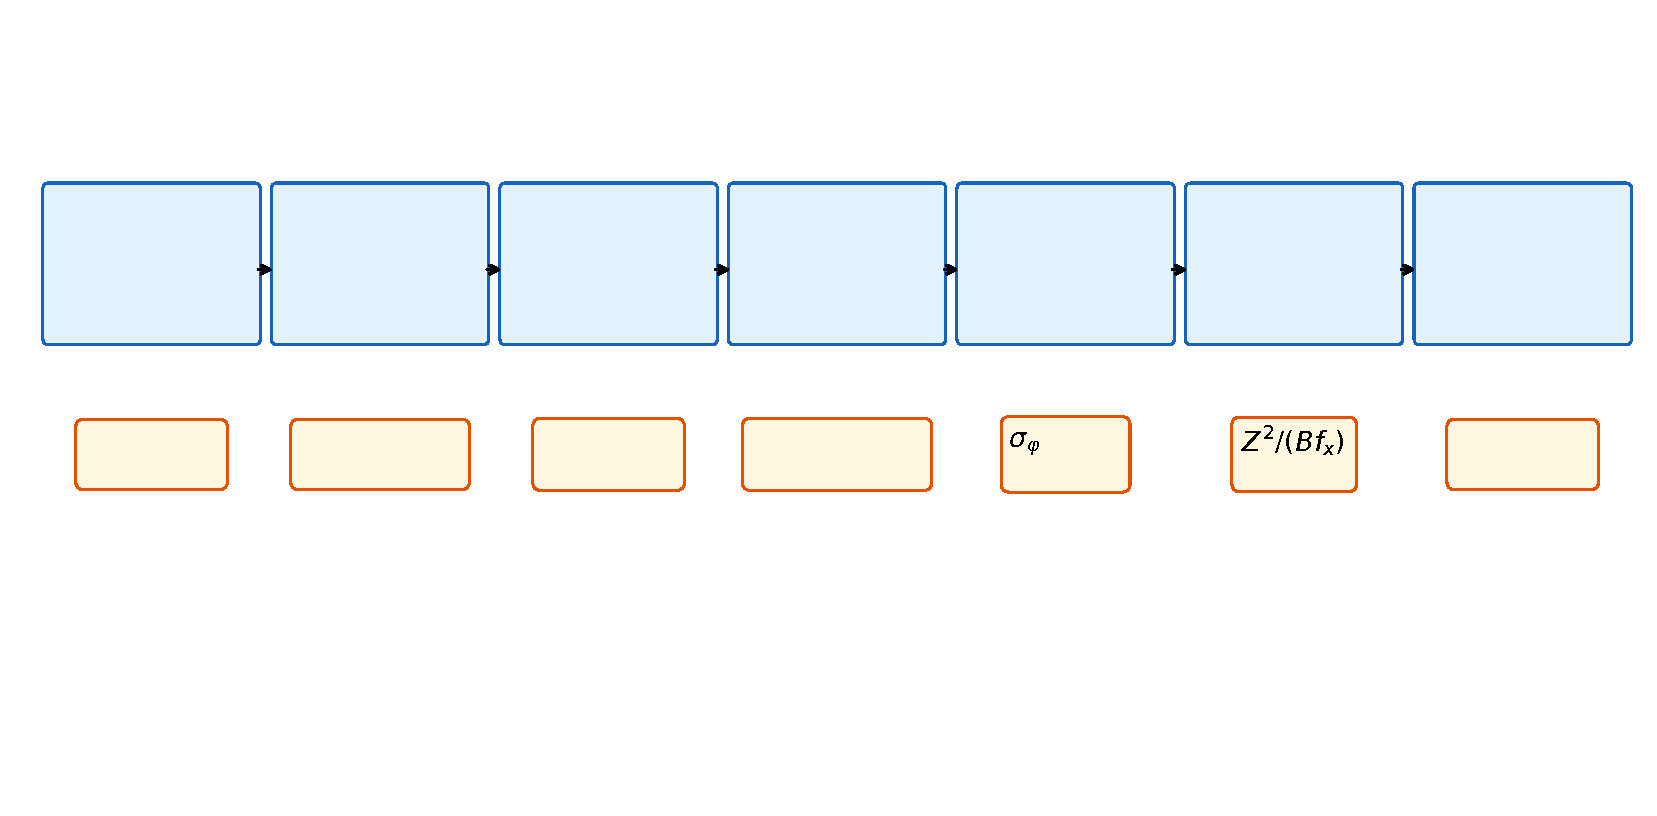
\includegraphics[width=\textwidth]{fig-error-budget-map.pdf}
  \caption{从光子到点云的误差链与各环节主要误差项、对应章节（概念草图，非精确工程图）。}
  \label{fig:ch11-map}
\end{figure}

\subsection{随机项与系统项}

\textbf{随机项}在重复测量间独立变化，均值为零：光子噪声、读出噪声、散斑（换照明位置后变化时）、量化噪声。它们按 $1/\sqrt{n}$ 随平均帧数 $n$ 降低，也随 $\SNR$ 提高而降低。

\textbf{系统项}在重复测量间保持不变，或随某个条件（深度、视场位置、材料、温度）确定性地变化：标定误差、残余畸变、伽马谐波、次表面散射偏置、色差、混合像素、展开错误。平均对它们无效；只能通过更好的模型（标定、补偿）、改变测量条件（换波长、换频率、交叉偏振），或改变设计来降低。

两点值得强调：
\begin{itemize}
  \item 同一现象可兼具两种成分。例如散斑：固定照明下对静止物体是系统项（每次都一样），移动照明或物体后变为随机项。
  \item 系统项常有\emph{空间结构}：碗形、周期波纹、台阶、尺度偏差。这一结构正是诊断的线索。
\end{itemize}

\subsection{误差合成}

相互独立的随机项按平方和合成：
\begin{equation}
  \sigma_{Z,\mathrm{rand}}=\sqrt{\sum_i\sigma_{Z,i}^{2}}.
  \label{eq:ch11-rss}
\end{equation}
系统项若方向与大小已知，应直接补偿；若只知道上界，保守做法是线性相加，较乐观的做法是视为未知但独立后按平方和合成。最终报告建议分开给出随机部分与系统部分，而不是只给一个数。

把各环节换算到深度，常用的「换算因子」是：
\begin{itemize}
  \item 灰度噪声 $\to$ 相位：$\sigma_\varphi\approx\sqrt{2/N}\,\sigma_I/M$（第~\ref{ch:07}~章）；
  \item 链路 $\MTF$ $\to$ 调制幅：$M\approx AV_0\MTF_{\mathrm{link}}$（第~\ref{ch:09}~章）；
  \item 相位 $\to$ 视差：$\delta d=\dfrac{P}{2\pi}\sigma_\varphi$（$P$ 为像面条纹周期，像素；相机–投影仪对中投影侧坐标由相位给出，视差误差即相机侧定位误差折算值）；
  \item 视差 $\to$ 深度：$\delta Z\approx Z^2\delta d/(Bf_x)$（第~\ref{ch:08}~章）；
  \item 标定尺度误差 $\to$ 深度：$\delta Z/Z=\delta B/B$ 或 $\delta f_x/f_x$（第~\ref{ch:08}~章）。
\end{itemize}

\subsection{一张示意误差预算表}

以下表格为一台口内结构光设备的数量级示意（不对应具体产品）：$Z=15\,\mathrm{mm}$、$B=8\,\mathrm{mm}$、$f_x=1500$ 像素、像面条纹周期 $P=16$ 像素、四步相移。

\begin{table}[htbp]
  \centering
  \small\setlength{\tabcolsep}{4pt}
  \begin{tabular}{@{}llllc@{}}
    \toprule
    环节 & 误差项 & 性质 & 深度贡献（量级） & 章 \\
    \midrule
    传感器 & 光子+读出噪声，$\sigma_\varphi\approx0.03\,\mathrm{rad}$ & 随机 & $\sim1.4\,\mu\mathrm{m}$ & \ref{ch:06}, \ref{ch:07} \\
    镜头 & 景深边缘 $\MTF$ 降至 $1/3$ & 乘子$^{\dagger}$ & $\times3$（$\to\sim4\,\mu\mathrm{m}$）  & \ref{ch:09} \\
    投影 & 伽马谐波残差 & 系统 & $2$--$5\,\mu\mathrm{m}$ & \ref{ch:07} \\
    场景 & 散射偏置 & 系统 & $10$--$40\,\mu\mathrm{m}$ & \ref{ch:07} \\
    场景 & 高反饱和区 & 系统/缺失 & 失效，需掩膜 & \ref{ch:05}, \ref{ch:07} \\
    镜头 & 残余畸变 & 系统 & $2$--$10\,\mu\mathrm{m}$ & \ref{ch:02} \\
    镜头 & 色差（标定波长不符） & 系统 & $\sim5\,\mu\mathrm{m}$ & \ref{ch:09} \\
    三角 & 基线标定 $\delta B/B=5\times10^{-4}$ & 系统（尺度） & $\sim7.5\,\mu\mathrm{m}$ & \ref{ch:08} \\
    三角 & 温漂 & 系统（慢变） & $5$--$20\,\mu\mathrm{m}$ & \ref{ch:08} \\
    场景 & 运动（$20\,\mathrm{mm/s}$，$8\,\mathrm{ms}$） & 系统（帧间） & 依补偿而定 & \ref{ch:07} \\
    点云 & 全牙弓拼接累积 & 系统（累积） & 数十--上百 $\mu\mathrm{m}$ & — \\
    \bottomrule
  \end{tabular}
  \par\smallskip\footnotesize $^{\dagger}$ 乘子作用于上一行的随机项（景深边缘处），不是独立误差项，不另计入平方和。
  \caption{误差预算示意（数量级示意，不对应具体产品）。}
  \label{tab:ch11-budget}
\end{table}

随机项计算示例：$\delta d=16\times0.03/(2\pi)\approx0.076$ 像素，$\delta Z\approx225\times0.076/12000\,\mathrm{mm}\approx1.4\,\mu\mathrm{m}$。表格的结论与第~\ref{ch:08}~章一致：\emph{单点随机噪声远不是瓶颈}，材料、标定与拼接等系统项主导。改进的优先级应按系统项从大到小排列。

\subsection{诊断检查清单：按症状反查}

\begin{table}[htbp]
  \centering
  \small
  \begin{tabular}{@{}p{0.36\textwidth}p{0.36\textwidth}c@{}}
    \toprule
    症状 & 最可能原因 & 章 \\
    \midrule
    平面重建为碗形或马鞍形 & 残余畸变、主点误差、色差 & \ref{ch:02}, \ref{ch:08}, \ref{ch:09} \\
    尺寸整体偏大或偏小（与位置无关） & 基线或焦距标定尺度误差 & \ref{ch:08} \\
    深度误差随深度非线性增长 & $Z^2$ 放大、视差偏置、景深外 & \ref{ch:08}, \ref{ch:01} \\
    与条纹同方向、间距一个周期的台阶 & 相位展开级次错误 & \ref{ch:07} \\
    频率为条纹 $N$ 倍的规则波纹 & 伽马、DMD 同步 & \ref{ch:07} \\
    与条纹同频的波纹，随移动速度增大 & 运动伪影 & \ref{ch:07} \\
    半透明材料上深度系统性偏低、细节被抹平 & 次表面散射 & \ref{ch:07}, \ref{ch:09} \\
    亮斑处空洞或噪点 & 镜面高反、饱和 & \ref{ch:05}, \ref{ch:06} \\
    边缘一圈漂浮点 & 混合像素 & \ref{ch:09}, \ref{ch:08} \\
    凹角处深度偏大、磨圆 & 互反射或多径 & \ref{ch:07}, \ref{ch:10} \\
    景深边缘噪声显著增大 & 离焦 $\MTF$ 降低 $M$ & \ref{ch:01}, \ref{ch:09} \\
    颗粒状、换位置即变的噪声 & 散斑 & \ref{ch:04}, \ref{ch:05} \\
    随开机时间缓慢漂移 & 温漂、光源亮度漂移 & \ref{ch:06}, \ref{ch:08} \\
    暗区噪声高、亮区正常 & 读出噪声主导、曝光不足 & \ref{ch:06} \\
    \bottomrule
  \end{tabular}
  \caption{症状反查清单。}
  \label{tab:ch11-checklist}
\end{table}

使用方法：先看误差的\emph{空间结构}（全局 / 随深度 / 随视场 / 周期性 / 局部材料相关），再看它是否随重复测量变化（随机还是系统），最后用对照实验（换标准件、换材料、静止与运动对比、换曝光）确认。

\subsection{例：从症状反查到修复，走一遍}

以下用前面各章算过的数，把检查清单（表~\ref{tab:ch11-checklist}）实际走一遍。场景为数量级示意：平面标准件扫描后，点云上出现与条纹方向平行的规则波纹，峰峰值约 $20\,\mu\mathrm{m}$，周期约为条纹周期的三分之一。

\begin{enumerate}
  \item \textbf{先分随机还是系统。} 对同一位置连拍十次取平均，波纹不变，只是颗粒噪声变小。结论：系统项。随机噪声来源（第~\ref{ch:06}~章）可以先放下。
  \item \textbf{看空间频率。} 波纹周期是条纹周期的 $1/3$，在相位域即 $3$ 倍频。第~\ref{ch:07}~章推出：$N$ 步相移的伽马误差是 $N$ 倍频波纹；自动曝光跳变的误差是基频与二倍频。因此首先怀疑三步相移的伽马残余。
  \item \textbf{定量核对。} 三步、伽马指数 $\Gamma=2.2$ 时误差峰值约 $0.23\,\mathrm{rad}$，对应 $\delta Z\approx11\,\mu\mathrm{m}$，峰峰值约 $22\,\mu\mathrm{m}$，与观测吻合。
  \item \textbf{设计验证实验。} 换四步相移再扫：若波纹降到 $1\,\mu\mathrm{m}$ 以下（四步伽马误差约 $0.3\,\mu\mathrm{m}$），诊断成立；若波纹频率变成 $4$ 倍频但幅度不降，说明非线性远比 $\Gamma=2.2$ 严重或来自别处。
  \item \textbf{修复与复验。} 两条路：保持三步，但测投影—相机灰度响应并做逆查找表预校正（残余 $\Gamma\approx1.1$ 时误差约 $0.022\,\mathrm{rad}$，约 $1\,\mu\mathrm{m}$）；或改四步，代价是多一帧、对运动更敏感。复验时仍用平面标准件，并在两种距离上测，以排除只在某个离焦量上成立的巧合。
\end{enumerate}
这次走查的要点不是伽马本身，而是顺序：先用平均区分随机与系统，再用空间频率把候选源缩到一两个，再用前面章节的公式核对幅度，最后用一个能证伪的实验验证。

\subsection{推导：多视图拼接的误差累积}

口扫全牙弓由数百帧逐帧配准拼接而成。设每对相邻帧的配准平移误差独立、标准差 $\sigma_t$，经 $n$ 次拼接后末帧相对首帧的平移误差为随机游走：
\[
  \sigma_{t,n}=\sqrt n\,\sigma_t .
\]
旋转误差更麻烦：每步旋转误差 $\sigma_r$ 累积为 $\sqrt n\,\sigma_r$，而它在距离 $L$ 处造成的位移为 $L\sqrt n\,\sigma_r$——杠杆臂越长，放大越大。

\textbf{数量级示意。} $\sigma_t=5\,\mu\mathrm{m}$，$n=100$：平移累积 $50\,\mu\mathrm{m}$。$\sigma_r=1.75\times10^{-4}\,\mathrm{rad}$（$0.01^\circ$），杠杆 $L=40\,\mathrm{mm}$：$1.75\times10^{-3}\times40\,\mathrm{mm}=70\,\mu\mathrm{m}$。两者合成约 $86\,\mu\mathrm{m}$，远大于单帧深度噪声（约 $1\,\mu\mathrm{m}$）。这解释了一个常见现象：单帧精度极好的设备，全牙弓尺寸误差仍可达数十微米，并且误差集中在扫描路径的末端（例如牙弓另一侧）。

适用条件与修正：上式假设误差独立；若配准误差有同号偏置（例如每步都偏向同一方向的尺度误差），累积随 $n$ 线性而非 $\sqrt n$ 增长，更糟。降低累积的手段：闭环（扫描路径回到起点，用首尾约束做全局优化，把误差分散到整条路径）；减少拼接次数（每帧视场更大）；或加入外部参考（已知尺寸的标记物）。

\subsection{用蒙特卡洛核对误差预算}

平方和合成（式~\eqref{eq:ch11-rss}）依赖两个前提：各项独立、线性化有效。二者都可能失效：外差跳级是非线性的粗大误差；伽马波纹与相位相关。蒙特卡洛是检查前提是否成立的直接办法：
\begin{enumerate}
  \item 用标定得到的模型生成一组「真值」相位图与几何；
  \item 每次试验按各误差源的分布独立抽样（光子噪声按泊松、读出噪声按高斯、标定参数按标定协方差），生成带误差的图像；
  \item 用与实际相同的流水线（相移解算、展开、三角化）重建；
  \item 统计重建与真值之差的标准差与分位数，与平方和预算比较。
\end{enumerate}
所需试验次数：标准差估计的相对误差约为 $1/\sqrt{2n}$，要 $1\%$ 精度需约 $5000$ 次。若关心的是跳级这类小概率事件，例如 $10^{-4}$ 量级，则每像素需要远多于 $10^4$ 次，或者把一张图的全部像素当作独立样本。

C++/CUDA 实现要点：每个线程负责一个（像素，试验）组合；用计数器型随机数生成器（如 cuRAND 的 Philox），以 $(\text{像素},\text{试验})$ 为种子偏移，保证可复现且线程间独立；尽量直接调用生产流水线的同一套核函数，而不是另写一份「简化版」，否则验证的是另一份代码。若蒙特卡洛结果比平方和大得多，通常提示存在非线性或相关项，应回到误差链逐项排查。

\section{限度}
\label{sec:ch11-limits}

\begin{itemize}
  \item 预算表的数值为量级示意，真实系统必须用标准件实测各项，尤其是材料相关的系统项。
  \item 平方和合成假设各项独立；实际中离焦、散射与 $M$ 下降相互耦合，需要整体实验验证。
  \item 线性化的误差传播在大误差（展开错误、饱和）处失效，这些应作为「失效模式」单独统计其发生率。
  \item 本书未展开点云处理（配准、融合、网格化）的误差，它们在全牙弓尺度上往往最大，需另行建模。
\end{itemize}

\section{对象}
\label{sec:ch11-object}

\textbf{一次完整的设计复盘（数量级示意）。} 设目标：单颗牙单帧误差 $\le20\,\mu\mathrm{m}$（RMS），全牙弓 $\le100\,\mu\mathrm{m}$。
\begin{enumerate}
  \item \textbf{几何}（第~\ref{ch:08}~章）：探头宽约 $20\,\mathrm{mm}$，取 $B\approx8\,\mathrm{mm}$、$Z\approx15\,\mathrm{mm}$；随机项约 $1$--$2\,\mu\mathrm{m}$，满足。
  \item \textbf{景深}（第~\ref{ch:01}~章、第~\ref{ch:09}~章）：深度范围 $\pm5\,\mathrm{mm}$ 要求较大 F 数；景深边缘 $M$ 下降为焦面的 $1/3$，随机项增至约 $4$--$5\,\mu\mathrm{m}$，仍满足；但展开可靠性需检查。
  \item \textbf{光源}（第~\ref{ch:05}~章、第~\ref{ch:09}~章）：蓝光 LED 加带通，降低色差与散射穿透，散斑弱；按工作波长标定。
  \item \textbf{条纹周期}（第~\ref{ch:07}~章、第~\ref{ch:09}~章）：按景深边缘链路 $\MTF$ 选周期，配合多频展开。
  \item \textbf{材料}（第~\ref{ch:05}~章、第~\ref{ch:07}~章）：交叉偏振抑制高反；散射偏置用材料相关的补偿或更高频条纹缓解；这是剩余最大的单帧系统项。
  \item \textbf{传感器}（第~\ref{ch:06}~章）：全局快门、锁定曝光、与投影帧同步；多曝光处理金属修复体。
  \item \textbf{标定与漂移}（第~\ref{ch:02}~章、第~\ref{ch:03}~章、第~\ref{ch:08}~章）：以标准件定期校验尺度，监控温度。
  \item \textbf{拼接}：全牙弓误差由累积主导，需要全局优化与参考特征，本书之外。
\end{enumerate}
复盘的结论通常是：单帧预算由材料与标定主导，全牙弓预算由拼接主导，光学随机噪声排在后面。

\section*{本章收束}
从光子到点云的每一环都有可以量化的误差项。随机项靠 $\SNR$ 与平均降低；系统项必须靠模型、标定、改变测量条件或改设计降低，并且它们有可诊断的空间结构。一张写清楚「项、性质、量级、章节」的预算表，加上一份按症状反查的清单，是设计、调试与评审三维重建系统的共同工具。

\section{习题}
\label{sec:ch11-exercises}

\begin{enumerate}
  \item \textbf{（计算）} 采用表~\ref{tab:ch11-budget} 的参数，若改用六步相移且灰度噪声不变，随机深度误差变为多少？对总误差有多大影响？
  \item \textbf{（计算）} 随机项 $4\,\mu\mathrm{m}$、伽马残差 $3\,\mu\mathrm{m}$、畸变残差 $6\,\mu\mathrm{m}$、散射偏置上界 $20\,\mu\mathrm{m}$。分别按平方和与线性相加合成，并讨论哪种更适合对外报告。
  \item \textbf{（重建场景）} 某设备扫描标准球：球面拟合残差 $5\,\mu\mathrm{m}$，但球心距比标称大 $0.3\%$。分别对应哪类误差？如何处理？
  \item \textbf{（重建场景）} 扫描一颗离体牙，釉质区与牙本质暴露区之间出现约 $30\,\mu\mathrm{m}$ 的「台阶」，而实物表面光滑连续。按检查清单给出诊断步骤。
  \item \textbf{（重建场景）} 同一模型，手持扫描比固定支架扫描噪声更大，且出现与条纹同频的波纹。指出环节、章节与两种对策。
  \item \textbf{（设计）} 为把单帧误差从 $20\,\mu\mathrm{m}$ 降到 $10\,\mu\mathrm{m}$，你可以：加大基线、增加相移步数、改为更短波长、引入交叉偏振、提高标定频率。根据表~\ref{tab:ch11-budget} 排出优先级并说明理由。
  \item \textbf{（综合）} 一位同事声称「我们的相机噪声降低了一半，所以精度提高了一倍」。用本章的随机/系统框架评价这一说法。
  \item \textbf{（综合）} 为一台新的结构光样机写出最少的验证实验清单（每项对应一类误差），并说明每项实验能分离出什么。
  \item \textbf{（推导）} 若每步配准平移有固定偏置 $b$ 加随机误差 $\sigma_t$，写出 $n$ 步后的均方根误差，并求偏置开始主导的 $n$。
  \item \textbf{（计算）} 正文拼接例中，若闭环优化把误差近似均分，使末端误差降为开环的 $1/2$，并把杠杆缩短到 $25\,\mathrm{mm}$，合成误差为多少？
  \item \textbf{（口扫场景）} 正文走查中，若观测波纹周期等于条纹周期（基频），幅度约 $5\,\mu\mathrm{m}$，按第~\ref{ch:06}~章自动曝光例，应首先怀疑什么？设计一个验证实验。
  \item \textbf{（医学重建）} 一套术中体表扫描系统的预算平方和为 $0.3\,\mathrm{mm}$，蒙特卡洛结果为 $0.8\,\mathrm{mm}$ 且分布有长尾。列出两种可能原因，并说明如何从分位数分辨它们。
  \item \textbf{（C++/CUDA 实践）} 说明为何用 Philox 之类计数器型生成器，而不是每线程各自维护一个顺序生成器状态；若需要 $10^4$ 次试验、$10^6$ 像素，估算随机数总量与显存组织方式。
\end{enumerate}

\section{习题讲解}
\label{sec:ch11-solutions}

\begin{enumerate}
  \item $\sigma_\varphi\propto\sqrt{2/N}$，六步比四步降为 $\sqrt{4/6}\approx0.82$ 倍，约 $1.1\,\mu\mathrm{m}$（焦面）或约 $3.3\,\mu\mathrm{m}$（景深边缘）。总误差由系统项主导，改善很小；而采集时间增加 $50\%$，运动风险上升。
  \item 平方和：$\sqrt{16+9+36+400}\approx21.5\,\mu\mathrm{m}$；线性：$33\,\mu\mathrm{m}$。散射偏置主导两种结果。对外报告宜分开给出随机部分与系统部分；不确定方向的系统项可按上界保守报告。
  \item 拟合残差为局部随机与形状误差（小）；球心距偏差是尺度误差，来自基线或焦距标定（第~\ref{ch:08}~章）。用已校准的标准件做尺度修正或重新标定。
  \item 症状为材料相关的系统偏置 $\to$ 次表面散射（第~\ref{ch:07}~章、第~\ref{ch:09}~章）。步骤：在同一位置涂薄层不透明涂层再扫，台阶消失即证实；比较不同条纹频率下台阶大小；检查调制幅 $M$ 是否在牙本质区较低。
  \item 运动伪影，第~\ref{ch:07}~章。对策：缩短采集序列（提高帧率、减少帧数）；运动估计与补偿。
  \item 优先：交叉偏振与材料散射补偿（针对最大系统项）、更短波长（减散射穿透与色差）、提高标定与温漂监控频率；其次才是加大基线与增加相移步数，因为它们只降随机项，而随机项已远小于目标。
  \item 噪声减半只使随机项减半。若系统项主导（如表~\ref{tab:ch11-budget}），总精度几乎不变。应拿出分项预算或用标准件实测证明。
  \item 示例：(1) 平面板多位置：畸变、主点、色差；(2) 量块台阶与球距：尺度；(3) 静止重复扫描：随机噪声；(4) 同一形状不同材料（涂层与不涂层）：散射与高反；(5) 不同移动速度：运动伪影；(6) 长时间开机重复：温漂；(7) 不同深度位置：景深与 $Z^2$ 放大；(8) 全牙弓模型与参考扫描：拼接累积。
  \item 偏置线性累积 $nb$，随机项 $\sqrt n\sigma_t$，均方根 $\sqrt{n^2b^2+n\sigma_t^2}$。两项相等时 $n=\sigma_t^2/b^2$。例如 $\sigma_t=5\,\mu\mathrm{m}$、$b=0.5\,\mu\mathrm{m}$，$n=100$ 后偏置就主导。
  \item 平移 $25\,\mu\mathrm{m}$；旋转 $1.75\times10^{-3}\times25\,\mathrm{mm}/2\approx22\,\mu\mathrm{m}$；合成约 $33\,\mu\mathrm{m}$。
  \item 基频（和二倍频）波纹指向自动曝光或照明帧间波动：四步时幅度约 $\varepsilon/(2V)$，$5\,\mu\mathrm{m}$ 约对应 $0.1\,\mathrm{rad}$，$V=0.5$ 时 $\varepsilon\approx10\%$。验证：锁定曝光与增益重扫；或记录每帧平均灰度看是否跳变。若锁定后波纹消失，诊断成立。
  \item (i) 存在非线性粗大误差，如展开跳级或混合像素：分布中心与预算一致，但高分位（$99\%$ 以上）远超高斯外推，呈长尾；(ii) 存在漏算或相关的系统项，如标定尺度误差：整个分布变宽，中位绝对误差也明显大于预算。比较中位与高分位相对高斯的比值即可区分。
  \item 计数器型生成器由（种子，计数器）直接算出随机数，无需存储和推进每线程状态，任意线程、任意试验可独立复现，也不受线程调度顺序影响。$10^{10}$ 个（像素，试验）组合，每组合若需每帧若干个随机数，总量在 $10^{11}$ 量级，不可能存储，应在核函数内即时生成；显存只存统计量（每像素的和与平方和，或直方图），按批次（例如每次 $100$ 次试验）累加。
\end{enumerate}


\backmatter
\bibliographystyle{plainnat}
\bibliography{refs/book}

\end{document}
